%% 
%% Copyright 2019-2020 Elsevier Ltd
%% 
%% This file is part of the 'CAS Bundle'.
%% --------------------------------------
%% 
%% It may be distributed under the conditions of the LaTeX Project Public
%% License, either version 1.2 of this license or (at your option) any
%% later version.  The latest version of this license is in
%%    http://www.latex-project.org/lppl.txt
%% and version 1.2 or later is part of all distributions of LaTeX
%% version 1999/12/01 or later.
%% 
%% The list of all files belonging to the 'CAS Bundle' is
%% given in the file `manifest.txt'.
%% 
%% Template article for cas-sc documentclass for 
%% double column output.

%\documentclass[a4paper,fleqn,longmktitle]{cas-sc}
\documentclass[a4paper,fleqn]{cas-sc}
% \usepackage[numbers]{natbib}
%\usepackage[authoryear]{natbib}
\usepackage[authoryear,longnamesfirst]{natbib}
\usepackage{float}
%%%Author definitions
\def\tsc#1{\csdef{#1}{\textsc{\lowercase{#1}}\xspace}}
\tsc{WGM}
\tsc{QE}
\tsc{EP}
\tsc{PMS}
\tsc{BEC}
\tsc{DE}
%%%

% Uncomment and use as if needed
%\newtheorem{theorem}{Theorem}
%\newtheorem{lemma}[theorem]{Lemma}
%\newdefinition{rmk}{Remark}
%\newproof{pf}{Proof}
%\newproof{pot}{Proof of Theorem \ref{thm}}

\begin{document}
\let\WriteBookmarks\relax
\def\floatpagepagefraction{1}
\def\textpagefraction{.001}

% Short title
\shorttitle{Microclimate spatio-temporal prediction}



% Short author
\shortauthors{Han et~al.}

% Main title of the paper
% \title [mode = title]{A spatio-temporal microclimate prediction model using deep learning and land use data} 
\title [mode = title]{Microclimate spatio-temporal prediction using deep learning and land use data}
% High-resolution spatio-temporal prediction  of microclimate using deep learning and land use data
% Title footnote mark
% eg: \tnotemark[1]

% Title footnote 1.
% eg: \tnotetext[1]{Title footnote text}
% \tnotetext[<tnote number>]{<tnote text>} 


% First author
%
% Options: Use if required
% eg: \author[1,3]{Author Name}[type=editor,
%       style=chinese,
%       auid=000,
%       bioid=1,
%       prefix=Sir,
%       orcid=0000-0000-0000-0000,
%       facebook=<facebook id>,
%       twitter=<twitter id>,
%       linkedin=<linkedin id>,
%       gplus=<gplus id>]
\author[1]{Han Jintong}[style=chinese,orcid=0009-0002-8394-6290]

% Corresponding author indication

% Footnote of the first author

% Email id of the first author
\ead{jintong@nus.edu.sg}

% URL of the first author
%  Credit authorship
\credit{Methodology, Software, Formal analysis, Investigation, Visualization, Writing - Original Draft}

% Address/affiliation
\affiliation[1]{organization={Department of the Built Environment, College of Design and Engineering, National University of Singapore},
    addressline={4 Architecture Drive}, 
    %city={Singapore},
    % citysep={}, % Uncomment if no comma needed between city and postcode
    postcode={117566}, 
    % state={},
    country={Singapore}}

% Second author

\author[1]{Adrian Chong}[orcid=0000-0002-9486-4728]
\ead{adrian.chong@nus.edu.sg}
\credit{Conceptualization, Methodology, Supervision, Writing - Review \& Editing, Funding acquisition}
\cormark[1]
% Corresponding author text
\cortext[cor1]{Corresponding author}

\affiliation[2]{organization={Institute for Infocomm Research, Agency for Science, Technology and Research (A*STAR)},
    % addressline={}, 
    % citysep={}, % Uncomment if no comma needed between city and postcode
    postcode={138632}, 
    country={Singapore}}

 \author[1]{Joie Lim}[orcid=0000-0002-4893-211X]
\ead{joie.lim@nus.edu.sg}   
\credit{Resources, Data Curation}

% Fourth author
\author%
[2]
{Savitha Ramasamy}[orcid=0000-0003-1534-2989]
\ead{ramasamysa@i2r.a-star.edu.sg}
\credit{Conceptualization, Methodology, Writing - Review \& Editing}



% Third author
\author[1]{Wong Nyuk Hien}[style=chinese, orcid=0000-0003-2964-7492]
\ead{bdgwnh@nus.edu.sg}
\credit{Resources}

% Address/affiliation


\author[3,4]{Filip Biljecki}[orcid=0000-0002-6229-7749]
% Corresponding author text
\ead{filip@nus.edu.sg}
\credit{Visualization, Writing - Review \& Editing, Project administration, Funding acquisition}
\affiliation[3]{organization={Department of Architecture, College of Design and Engineering, National University of Singapore},addressline={4 Architecture Drive}, postcode={117566},country={Singapore}}
\affiliation[4]{organization={Department of Real Estate, Business School, National University of Singapore},addressline={15 Kent Ridge Drive}, postcode={119245},country={Singapore}}
% Footnote text


% For a title note without a number/mark


% Here goes the abstract
\begin{abstract}
Urban microclimate prediction has significant importance across various fields, including Building Performance Simulation (BPS), outdoor thermal comfort, building life cycle, and residential health. Existing methods involve using classical weather file data, such as Typical Meteorological Years (TMY), or machine learning techniques for time-based forecasting. However, the incorporation of both spatial and temporal dimensions and land use/land cover (LULC) data is seldom considered. This paper proposes a novel approach to predict microclimate: the Geo-LSTM-Kriging model, which is applicable for fine-scale microclimate prediction within a few hundred meters around weather stations. The Geo-layer processes and learns from LULC data, the LSTM layer extracts and learns information from historical data, and the Kriging layer extracts spatial distance information. This comprehensive combination integrates spatial, temporal and environmental conditions, providing more accurate and detailed results with a higher spatial resolution (1 m $\times$ 1 m) and shorter time intervals (10 min) for microclimate prediction. These prediction results were achieved by employing statistical downscaling calculation and utilizing data from 14 weather stations located within the campus of our university. Upon the analysis of these prediction results, we found that the proposed model can accurately predict temperature and humidity at high spatial and temporal resolution. Compared to traditional interpolation models, the RMSE of temperature reduces from 1.59 ° C to 0.64 ° C and the RMSE of relative humidity (RH) reduces from 7.70 to 3.23. Through a comprehensive analysis of the model results, we have also identified varied impacts on microclimate predictions associated with different LULC features. These results demonstrate the value of the proposed model in microclimate prediction and attest to the benefits of incorporating LULC data. 
\end{abstract}

% Use if graphical abstract is present
% \begin{graphicalabstract}
% \includegraphics{figs/grabs.pdf}
% \end{graphicalabstract}

% Research highlights
\begin{highlights}
\item Microclimates could exhibit noticeable variations within small spatial and temporal scales.
\item Combining spatial and temporal knowledge contributes to the microclimate prediction accuracy.
\item Integrating LULC data enhances the stability of prediction errors.
\item Different LULC features have varying temporal effects on microclimate predictions.
%\item The Kriging layer exhibits the most prominent improvement among all layers in the entire Geo-LSTM-Kriging model.
%\item The integration of geographical knowledge presents a unique opportunity for future research.
\end{highlights}

% Keywords
% Each keyword is separated by \sep
\begin{keywords}
Microclimate Prediction  \sep Interpolation  \sep LSTM \sep Kriging \sep Urban morphology 
\end{keywords}


\maketitle

\section{Introduction}\label{Introduction}

The proportion of the world's population in urban areas has increased significantly over the past decade. It is predicted to exceed 70\% by 2050, according to a report by the United Nations \citep{nations2019world}. Built environment and human activity have led to the urban heat island (UHI) effect \citep{arnfield2003two, akbari2016local,chakraborty2021reduction}. This effect leads to higher temperatures compared to less urbanized areas, significantly contributing to global warming, heat-related deaths, and unpredictable climate variations \citep{deilami2018urban}. Recently, there has been an increased interest in research investigating the relationship between human activities and the surrounding environment, in an attempt to mitigate the UHI effect that negatively affects the built environment and its climate. Urban microclimate, pertaining to the immediate atmospheric conditions surrounding buildings distinguished from the broader urban climate \citep{wang2021benchmarking}, has gained significant attention in this regard \citep{yang2023urban}.

Previous studies have utilized experimental and mathematical methods to demonstrate how microclimate features (e.g.\ temperature, humidity) influence building energy systems \citep{bijarniya2020environmental, im2022impact}, including air conditioning systems and solar power systems \citep{bevilacqua2020seasonal,wu2022revealing}. In the outdoor thermal comfort field, \citet{zhang2022assessment} confirmed that microclimatic factors have a similar impact on outdoor thermal comfort as macroclimate factors, and therefore microclimate factors are particularly important for outdoor thermal comfort in regions with disadvantageous macroclimates. Some studies have explored the impact of various parameters within microclimates on the physical health of residents \citep{wu2020impact,heidari2020effects}. \citet{hayles2022quantifying} found that the microclimate changes in precipitation and humidity have a significant impact on the service life of building materials. Gaining accurate knowledge and predicting various indicators of local microclimates can be beneficial for extensive research on microclimate impacts. In summary, characterizing the local microclimate has different applications in improving building performance, building material life-cycle, occupant health, and thermal comfort. Under constantly changing climate conditions, the prediction of microclimates becomes increasingly crucial.


%Therefore, studying and predicting the profile of urban microclimate is vital for built environment studies. 

%Some studies have explored the impact of various parameters within microclimates on the physical health of residents \citep{wu2020impact,heidari2020effects}. \cite{hayles2022quantifying} found that the microclimate changes in precipitation and humidity have a significant impact on the service life of building materials. In summary, the characteristics of a local microclimate, including various weather features, are utilized for different types of applications in building energy performances, building' lifecycle, residents' health, and thermal comfort.

However, various features of the microclimate may exhibit significantly different performances and drastic fluctuations within a very small spatial and temporal range. In Figure \ref{FIG:weatherData14pm}, we have compiled the changes in temperature and humidity for one hour from 14 weather stations within the scope of this study, which is a  1.9 km $\times$ 1.6 km urban area, as shown in Figure \ref{FIG:map}. The data represent the statistical results of minute-by-minute data within one hour. In Figure \ref{FIG:weatherData14pm}, the red numbers represent the standard deviation of temperature and humidity among different weather stations within one hour. We can observe fluctuations not only between adjacent weather stations but also within the same station, with standard deviations of temperature reaching approximately 2°C and standard deviations of RH reaching 7\% within one hour. However, existing research on microclimate prediction often overlooks this aspect. There are two relatively obvious gaps here: (1) the lack of microclimate data at high spatial and temporal resolution; (2) the need for more targeted predictions by incorporating contextual spatial data such as land use/land cover (LULC). In the meanwhile, many studies have demonstrated the influence of LULC on microclimate data. \citet{estoque2017effects} demonstrated that the mean temperature of the impervious surface is about 3 °C higher than that of the green space. However, there is still a lack of research that integrates land use in predicting the urban microclimate indicators at high spatial and temporal resolution. Therefore, this paper has the following two objectives:
\begin{itemize}
\item{To provide downscaling temperature and humidity data at a high spatial resolution and short temporal intervals that are sufficient for micro-climate-related studies.}
\item{To develop a model that considers the surrounding environmental conditions and further enhances the model performance based on existing algorithms.}
\end{itemize}

\begin{figure}[!h]
	\centering
        	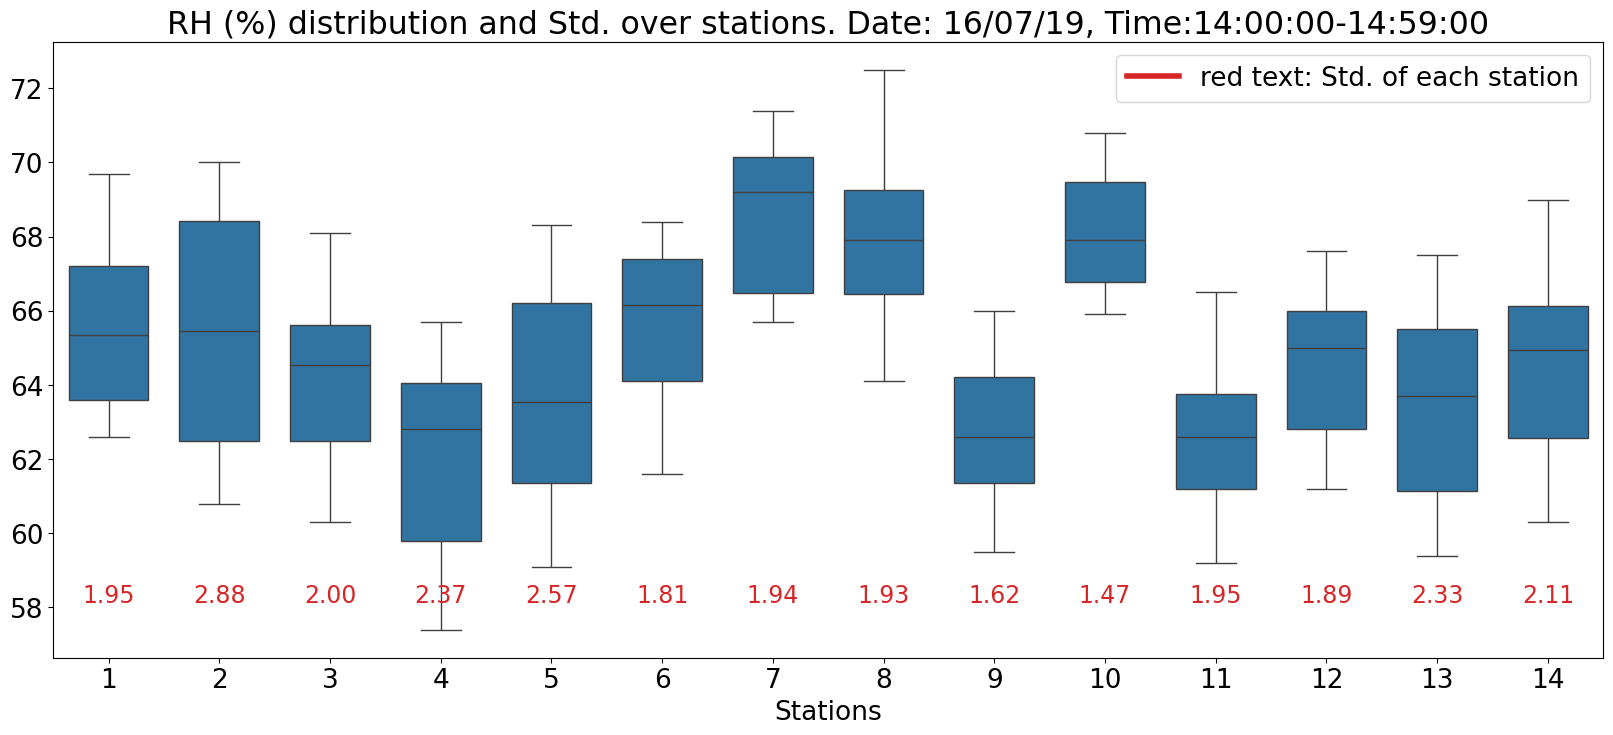
\includegraphics[scale=0.38]{figs/new_figs/RH14pm.png}
	    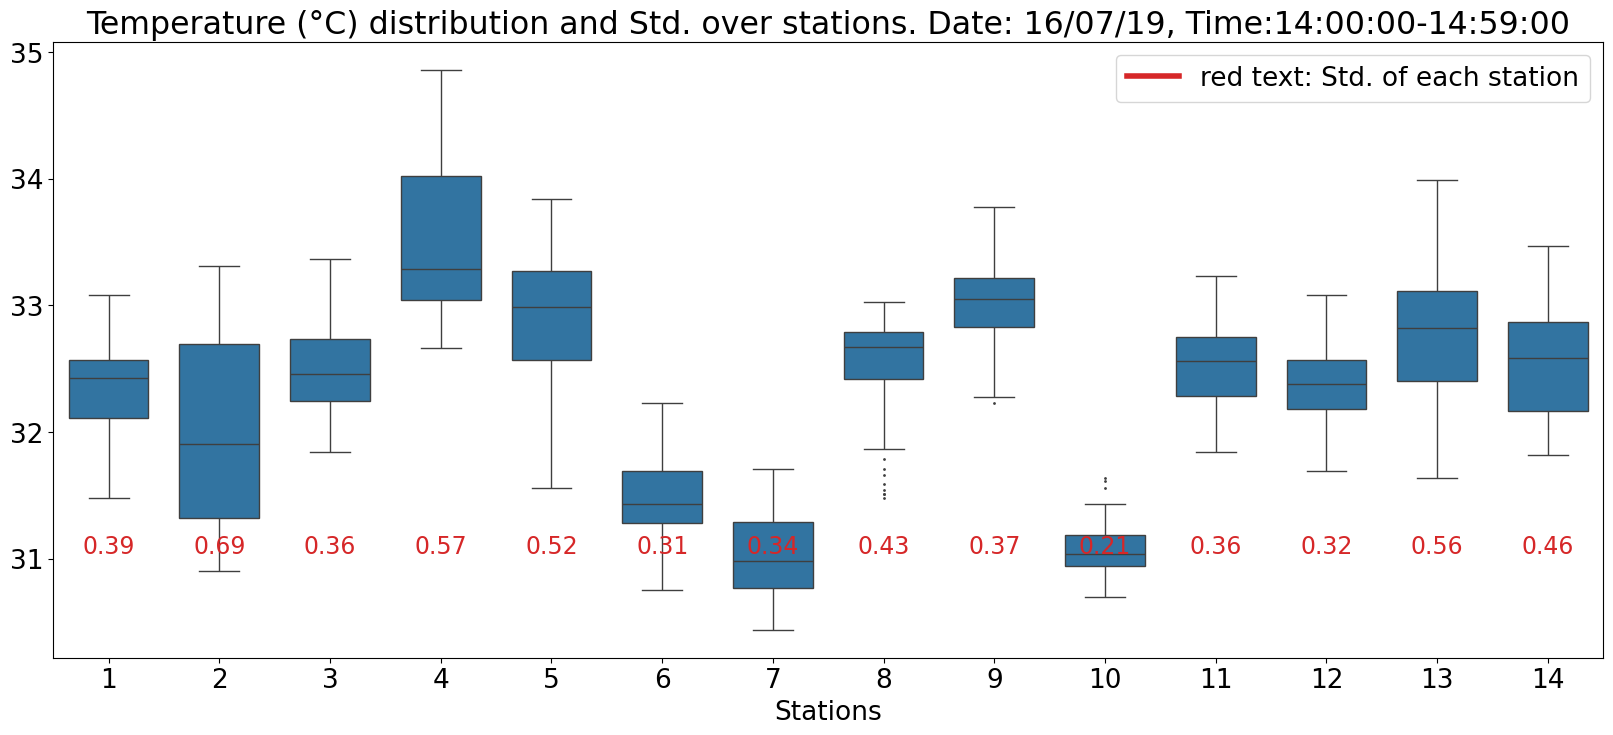
\includegraphics[scale=0.38]{figs/new_figs/tem14pm.png}
	\caption{Temperature and Relative humidity changes within one hour in the research area.}
	\label{FIG:weatherData14pm}
\end{figure}

\begin{figure}[!h]
	\centering
	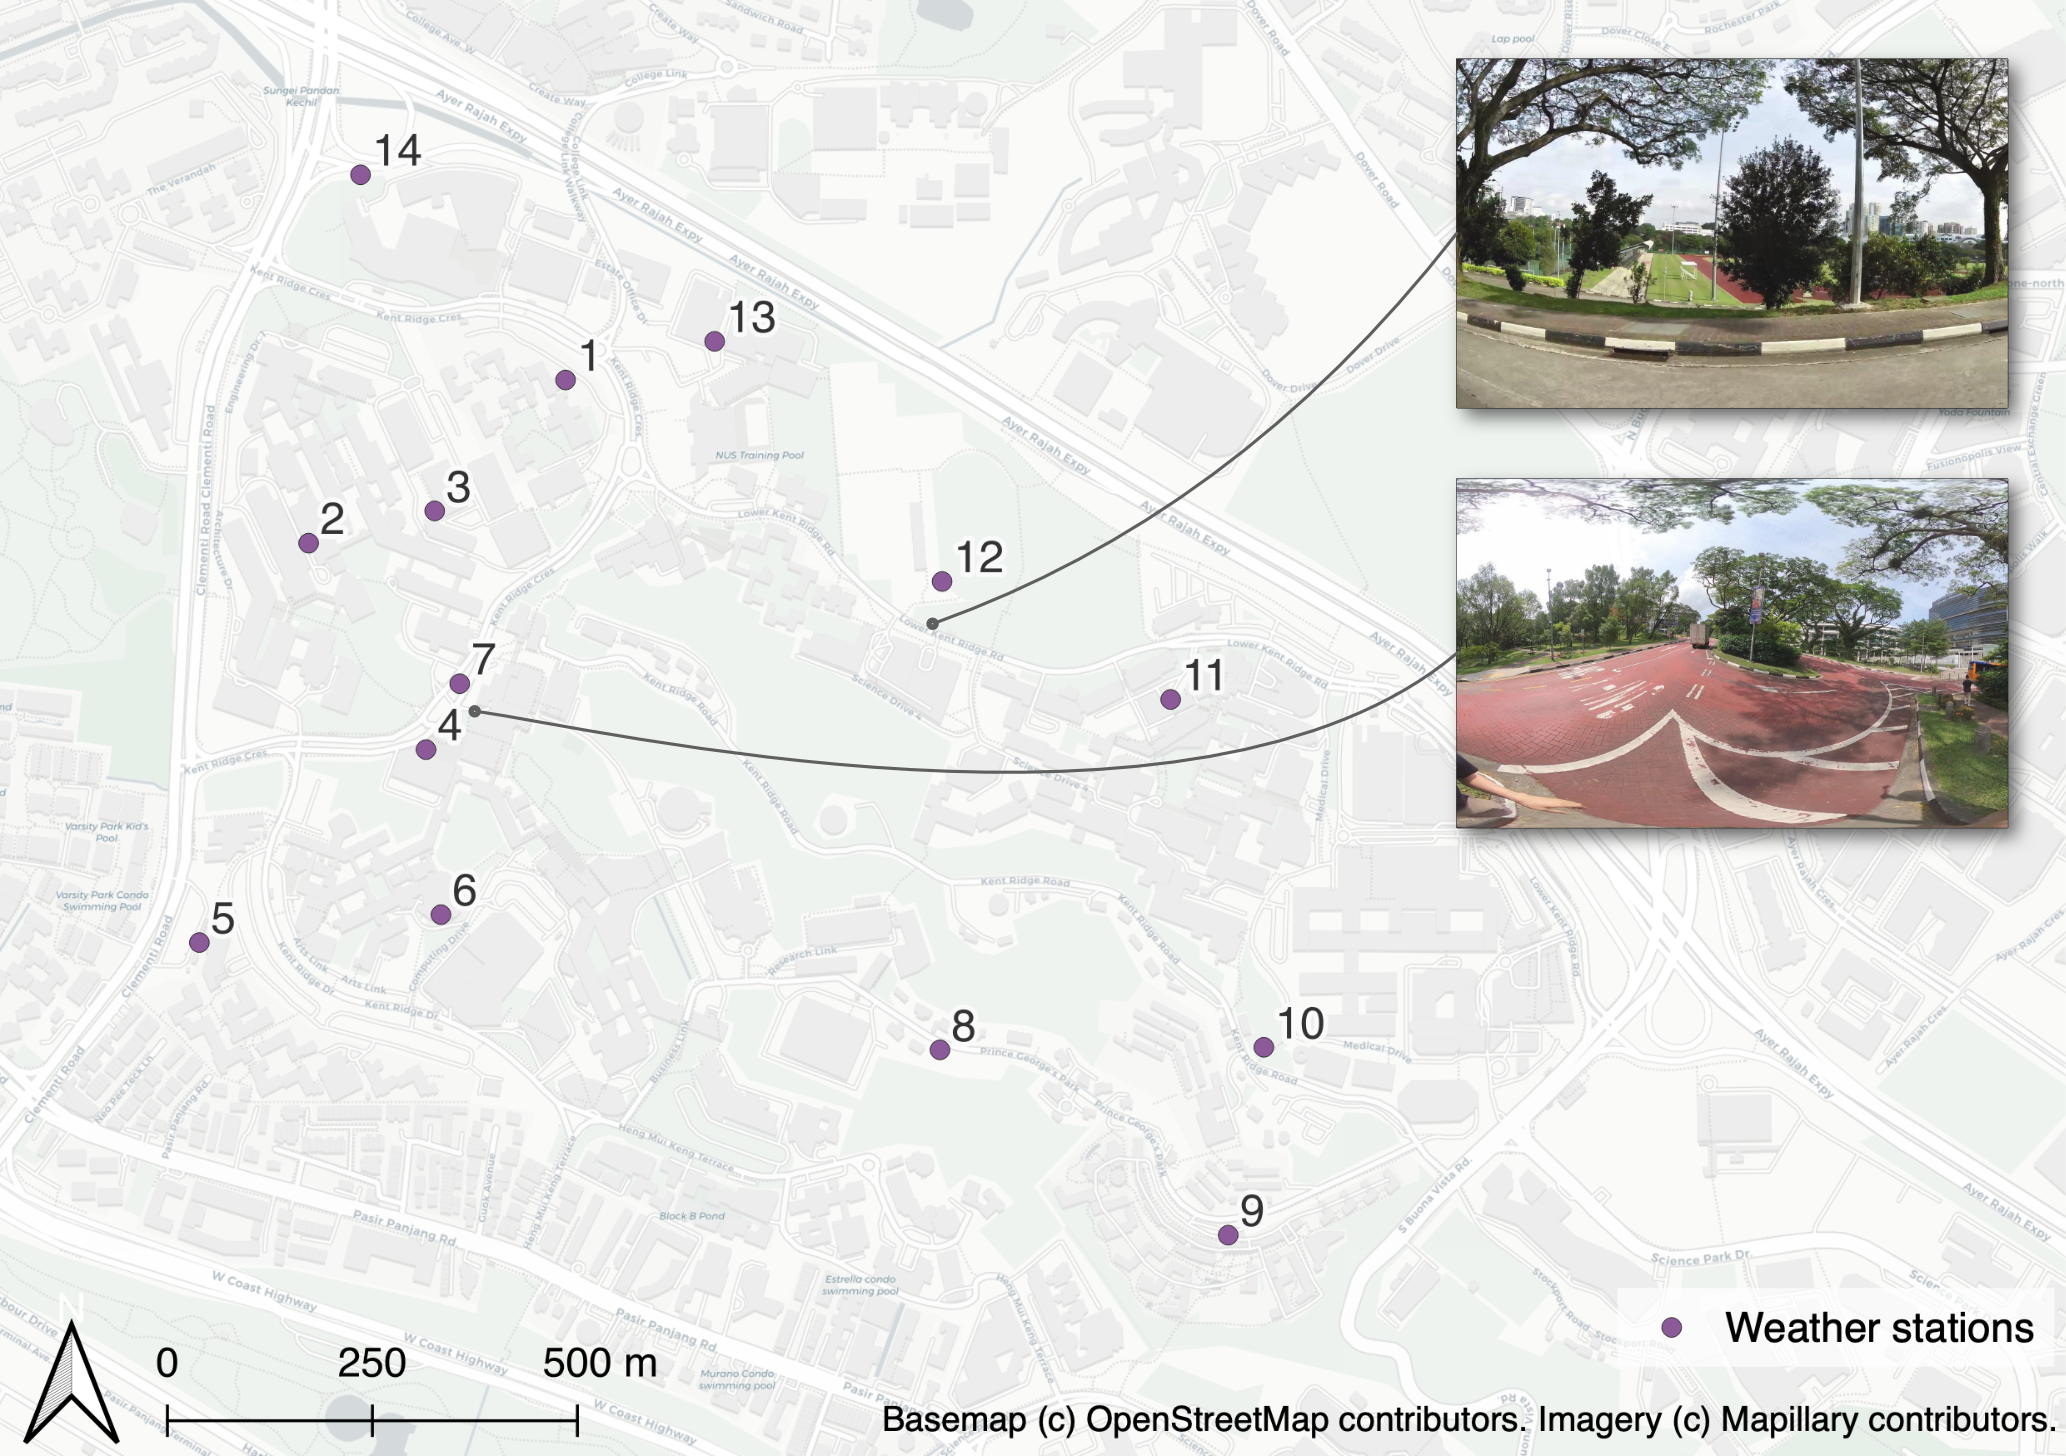
\includegraphics[width=.95\textwidth]{figs/map2_.png}
	\caption{The positions of weather stations whose data are used in model training, together with street-level imagery showing the streetscape in the study area.}
	\label{FIG:map}
\end{figure}

To achieve the aforementioned objectives, this paper proposes a Kriging-based LSTM neural network model combined with geographical land use data, which is called Geo-Kriging-LSTM, to estimate temperature and RH for the locations without weather stations or sensors. 
The rest of the paper is organized as follows: in Section \ref{Related Work}, an extensive examination of previous studies on microclimate prediction is presented, encompassing a range of methodologies. Section \ref{Methodology} illustrates the structure of the model and the inferences of the network, including the overview and verification of the data sources. Then in Section \ref{Results}, the experiment results are displayed and evaluated. Sections \ref{Discussion} and \ref{Conclusion} discuss the significance and conclude this study.

%aim: high spatial resolution of urban microclimate incorporating (land use)
 %how land use impact microclimate (beginning)
 %gap: spatial information, assume the weather station (validation perspective)

\section{Related Work}\label{Related Work}

In this section, we will provide existing research relevant to the following two main aspects: the impact of microclimate data on a wide range of studies, and commonly used microclimate prediction methods. Among these prediction methods, they are categorized into temporal methods, spatial methods, and spatio-temporal combined methods.

\subsection{Impact of microclimate}

Studying and predicting the variation of the urban micro-climate variables in space and time is vital for various studies. In building performance simulation, weather data forms the boundary condition for energy calculations and daylight analysis. Existing studies often utilize typical weather files such as the Weather Year for Energy Calculation 2 (WYEC2) and the Typical Meteorological Year (TMY) \citep{han2021using}. However, typical weather files lack a precise depiction of the microclimate conditions specific to the local area. Past studies have highlighted notable distinctions in temperature, humidity, and other variables between weather files data, urban climate stations, and adjacent microclimate stations \citep{wang2021benchmarking,lazos2014optimisation}. \cite{hosseini2017energy} undertook an extensive building performance simulation to investigate the impact of weather uncertainty on building energy estimation in Montreal, Canada, showing variances ranging from 3\% to 29\% in energy consumption when comparing simulations using actual weather data versus TMY2 data. 

In the field of outdoor thermal comfort, \citet{zhang2022assessment} confirmed that microclimate factors have a similar impact on outdoor thermal comfort as macroclimate factors. \citet{vinayak2022impacts} reveals that future increases in temperature in microclimates could result in 20\% Mumbai Metropolitan Region experiencing outdoor thermal discomfort. \cite{lin2021integrating} determined that incorporating microclimate information into urban landscape design can create outdoor environments with enhanced thermal comfort. \cite{zhang2022impact} explored the interaction mechanism among building spatial morphology, urban microclimate, and thermal comfort, indicating that geographical factors, such as urban vegetation, further influence outdoor thermal comfort by affecting various microclimate characteristics. 

Microclimate conditions also have an impact on different facets, such as residents' health. \cite{schinasi2018modification} summarized the association between microclimate indicators and epidemiologic and found that people living in hotter areas within cities had a 6\% higher risk of mortality/morbidity compared to those in cooler areas. \cite{zeren2023geographic} demonstrates a strong positive correlation between microclimate indices, particularly land surface temperature (LST), sleep deprivation, and heat stress among residents. \cite{alimukhamedov2022hygienic} assesses the health effects of microclimate indices on workers and finds that these conditions have a greater impact on male workers than on female workers. Moreover, adverse microclimate conditions have varying degrees of influence on the cardiovascular, respiratory, and urinary systems of both genders.

%Microclimate indicators, especially temperature and humidity, also have varying degrees of influence on the lifespan of building envelope and materials. 

Therefore, having accurate knowledge and predicting various indicators of local microclimate is beneficial for extensive research on microclimate. From the above references, we can also observe that wind speed, mean radiant temperature, air temperature and humidity are widely employed indicators in microclimate analysis. This study will focus on two of them, which are air temperature and relative humidity. 

\subsection{Microclimate prediction methods}

In macroscopic terms, microclimate prediction methods can be categorized into three main types: methods that utilize historical data for temporal prediction, methods that use neighboring spatial data for prediction, and hybrid methods that combine both temporal and spatial data for prediction.

\subsubsection{Temporal prediction methods}

The majority of microclimate prediction methods are based on historical data. To anticipate the characteristics of the urban microclimate, the prevailing approach often involves two categories: mathematical modeling, including Numerical Weather Prediction (NWP) models, and artificial neural network approaches. Employing mathematical modeling techniques often encompasses mass and energy balances. \cite{quemada2021simple} put forward a straightforward mathematical model aimed at estimating the annual maximum and minimum daily environmental temperatures. Such generalized mathematical models often have limitations in their ability to predict within larger spatial scales, and their predictions typically represent characteristic values, such as maximum or minimum values, over a given period. NWP models are built upon the fundamental principles of weather physics and account for the boundaries and environmental conditions associated with weather phenomena \citep{mathiesen2011evaluation}. NWP is capable of providing more accurate and detailed predictions, but it comes with the trade-off of higher computational costs to model the atmospheric system \citep{aggarwal2013comprehensive}. \cite{di2020mean} used NWP to predict global-scale mean radiation temperature (MRT). Within the scope of microclimate, their study obtained weather data predictions with a spatial resolution of 2.5 $\times$ 2.5 km using NWP.  However, for more detailed investigations into building performance or outdoor thermal comfort, the spatial resolution is insufficient. 
% data-driven methods

Alternatively, with the rapid development of artificial intelligence technology, machine learning methods are increasingly being applied in microclimate prediction. These methods commonly used can be broadly categorized into two types: Feed-forward Neural Networks (FFNN) and Recurrent Neural Networks (RNN). FFNN are data-driven predictive models that rely on data to capture and represent complex, non-linear patterns in large-scale weather datasets. \citet{bile2022novel} utilized FFNN to predict the short-term temperature trends inside museums, aiming to provide preventive measures for the protection of cultural artifacts. \cite{xie2022backpropagation} applied an FFNN model to predict the mean radiant temperature surrounding buildings. FFNNs offer benefits such as reproducibility, time-efficiency, and scalability, allowing them to be easily adapted to different temporal resolutions \citep{mocanu2018scalable}. RNNs are designed for time series data, and they have the ability to capture temporal dependencies and retain information from historical data. In addition to the basic RNN architecture, LSTM (Long Short-Term Memory) is another type of network developed based on RNN, and GRU (Gated Recurrent Unit) is a further simplified network based on LSTM \citep{zargar2021introduction}. \citet{zhang2021urban} used Long Short-Term Memory (LSTM) models for microclimate prediction and investigated their influence on buildings with different geometric configurations. \cite{koc2021investigation} used LSTM to predict temperature, showcasing the effectiveness of LSTM for climate prediction. However, research on utilizing RNNs for climate prediction studies is still relatively nascent in the built environment-related domains \citep{han2021using}.

%\cite{arulmozhi2021machine} employed various machine learning models, such as Random Forest and Support Vector Machine (SVM), to predict the temperature and humidity of indoor microclimates.   \cite{chang2021development} developed an Urban Micro-scale Temperature Forecasting (UMTF) model using K-means clustering and SVM, significantly reducing the mean absolute error by 1.0 degrees Celsius.  \cite{yang2019hourly} proposed a Fourier-series-based method to evaluate and forecast hourly air humidity fluctuations at different monitoring stations with satisfying results. 

%To address this research gap, this study aims to explore methods for obtaining high-resolution weather data from the perspective of spatial interpolation. By employing spatial interpolation techniques, the study seeks to enhance the resolution of weather data, allowing for a more accurate and detailed analysis of microclimate conditions.

\subsubsection{Spatial prediction methods}

There are various methods for spatial microclimate prediction. In general, researchers typically use standard weather file data as a baseline and employ different methods for downscaling calculations. There are two main approaches to downscaling weather data files: dynamical and statistical downscaling. The dynamical downscaling approach involves the utilization of physical models to simulate future weather, yielding data with higher resolution and enhanced reliability. Computational Fluid Dynamics (CFD) models are commonly used to simulate wind flow in urban areas, which can resolve the transfer of heat and mass and their interaction with individual obstacles, such as buildings \citep{toparlar2017review}. With the development of CFD and other physical-based microclimate models, an increasing number of studies have employed these models as predictive methodologies. \cite{crank2018evaluating} tested the air temperature perturbations using ENVI-met (a high-resolution 3D microclimate simulation software) with different vertical grid resolutions (0.75 to 2.0 m) and found that ENVI-net performs robustness when changing the vertical resolution. \cite{maronga2015parallelized} algorithmically optimized the Parallelized Large-Eddy Simulation Model (PALM), enabling it to perform computationally intensive simulations of meteorological data at large spatial scales and very high grid resolutions. \cite{moradi2021vertical} adopted and validated the Vertical City Weather Generator (VCWG) model (an efficient urban microclimate physics model) to assess its predictive performance within urban area, they found that the model is capable of accurately forecasting temperature, humidity, wind speed, and other variables in three-dimensional space. We can observe that such physics-based models generally exhibit higher accuracy and denser spatial resolution. However, it is equally true that, being based on physics-based meteorological models, they often require higher computational costs and a more accurate representation of topographical conditions within the specific scope \citep{p2021comparative}. 

On the other hand, the statistical downscaling is a simpler approach that establishes statistical connections between observed local climate variables and large-scale climate variables \cite{bamdad2021future}. Although statistical downscaling has the advantage of computational speed, its accuracy may be inferior compared to the computationally intensive dynamical downscaling method. \cite{aliabadi2023vatic} introduced the Vatic Weather File Generator (VWFG), a model capable of predicting weather conditions for the next 80 years based on records from the past 20 years. The ability to generate long-term future weather files aids in forecasting the energy consumption demands for heating and cooling in urban buildings. As illustrated in their study, such statistical downscaling methods typically rely on archives of TMY data, which are then adjusted based on commonly used regional or global climate models. These methods are more commonly employed for long-term climate trend predictions, lacking a perspective on shorter time intervals, and exhibiting a higher dependency on climate models and weather files. Meanwhile, we observe that interpolation methods are seldom mentioned in downscaling approaches, despite their ability to utilize localized meteorological station data for more direct and targeted downscaling computations.

Traditional spatial interpolation techniques can generally be categorized into deterministic methods (such as Triangular-based interpolation \citep{watson1984triangle}, Inverse Distance Weighted (IDW) \citep{bartier1996multivariate}, and Trend Surface Analysis (TSA) \citep{agterberg1984trend}, Spline interpolation \citep{schoenberg1973cardinal}), geostatistical methods (such as Kriging), and hybrid methods (such as Regression Kriging) \citep{granville2023selection}. In traditional interpolation methods, the most commonly used ones are IDW, Kriging, and Regression Kriging (RK) \citep{li2011review}. Among them, Regression Kriging is the combination of multivariate regression and Kriging and has been proven to have better interpolation performance in numerous instances. \cite{meng2013assessment} compared seven GIS interpolation methods and demonstrated that RK has the potential to significantly improve spatial prediction accuracy even when using a weakly correlated auxiliary variable. \cite{gia2019application} used different interpolation methods to estimate soil soil properties and observed that RK and Kriging exhibited respective advantages in various components, yet RK demonstrated superior performance in a majority of scenarios. \cite{azawi2021review} used different interpolation methods to estimate groundwater quality and found that RK yields higher accuracy.

Some other studies also applied machine learning methods to interpolation models. \cite{Kartal2022prediction} designed a hybrid method that combines the spatial interpolation approach with artificial neural networks, achieving MAE of 2.85\textdegree C using their NN-ConcLSTM model. \cite{imanian2023spatial} used deep learning approaches to overcome the weakness of the spline method when predicting the land-water interface temperature, reducing the RMSE by 16.2\%. 

We can observe that in addition to traditional interpolation methods, most recent studies choose to combine spatial interpolation with machine learning models to address the demand for higher spatial resolution. In this study, we combine spatial interpolation with time series prediction and also utilize the assistance of RNN models to achieve the same goal. The classic and broadly applied interpolation methods mentioned above will serve as baselines in this study. In summary, we utilized the machine learning methods with the incorporation of both temporal and spatial information.

\subsubsection{Incorporating land use/land cover (LULC)}

Land use/land cover (LULC) has been of great importance all over the world for many years. Land use encompasses the themes, purposes, duration, and spatial aspects of land utilization, while land cover primarily includes the types and properties of surface features on land \citep{nedd2021synthesis}. Many studies have demonstrated the significant impact of LULC on urban microclimate indicators. With the rapid development of human society, the influence of LULC on microclimate is increasing and shows no signs of diminishing due to the incrementally active, diverse, and internationalized human activities \citep{caballero2022land, naikoo2022land,abdullah2022investigating}. \cite{zhang2022impact} investigated the impact of LULC on microclimate and found a strong correlation between temperature, humidity, and specific building morphology parameters such as sky view factor, floor area ratio, site coverage ratio, and building storeys \citep{wei2016impact}. \cite{erell2022effect} found using microclimate simulations that increasing vegetation coverage can lead to a decrease of 0.3\textdegree C in annual average temperature. Consequently, incorporating LULC data in microclimate predictions could improve prediction performance. \cite{chang2021development} employed data-driven machine learning techniques in conjunction with LULC data to develop a 50 $\times$ 50 m grid-based temperature forecast for extreme events on the Kowloon Peninsula in Hong Kong, their results show that the statistical downscaling process reduced the model MAE by 1.03\textdegree C to 0.3\textdegree C for the maximum and minimum local temperature prediction. \cite{ma2019temporal} introduced a novel spatial interpolation/extrapolation methodology, called Geo-LSTM, to produce the spatial distribution of air pollutant concentrations, which integrates the spatial-temporal correlation from other monitoring stations.  However, there is still a scarcity of studies integrating LULC for microclimate prediction, especially for studies requiring high spatial resolution microclimate data, which warrants further research.

%The profile of urban microclimate is an essential input for myriad applications, for example, building energy modeling and daylight analysis.

%Nevertheless, 
%the optimization of the built environment generally requires various aspects of data, for example, energy consumption data \citep{reynolds2018zone,gao2010using}, pollution data \citep{brimblecombe2003effects,zhou2019spatial,wieser2021challenges}, natural environmental conditions \citep{guo2015study,omar2018optimization}, etc. 
%Weather data is one of the most intuitive and influential indicators for the study of the urban environment, built environment, and outdoor thermal comfort, especially in the micro-climate range. For example, \cite{kruger2013urban} investigated the outdoor comfort ranges in the Glasgow region of the UK, and collected thermal comfort data from respondents as they traveled along a designated route. However, the temperature data was obtained by the two weather stations as substitutes, rather than the actual data along the route. The issue of coarse weather data is not limited to this study, it is a common challenge in many outdoor thermal comfort research endeavors. When developing thermal comfort models for outdoor environments, many studies utilize standard weather files \citep{kruger2013assessment,kruger2017identifying,li2020perception} or a limited amount of data points from nearby weather stations as a substitute \citep{kruger2013urban,imbert2018simulation}. Research in the field of urban environment and building energy also encounters similar challenges, many scholars integrate and refine existing weather files to estimate the actual weather data \citep{liu2017comparing, p2021comparative}. In summary, weather data plays a crucial role in research related to building environments, nonetheless, currently available weather data is often insufficient in terms of spatial resolution.

%However, high-resolution microclimate data is not easily accessible on an urban scale because data collection often relies on a limited number of immobile weather stations and sensors, which can only provide data from scattered and distant geographical locations in most real cases. Weather data is therefore challenging to obtain for locations without established weather stations. Increasing the number of weather stations is possible but expensive. Under realistic conditions, the prediction and interpolation is a more feasible methodology. Microclimate prediction could learn from historical data and provide future weather conditions, enabling adaption to various changes, while interpolation could provide an estimation of new data points depending on the range of a discrete set of known data points \citep{britannica1993encyclopaedia,steffensen2006interpolation}. 

%There are two main approaches to weather prediction: numerical (dynamical) forecasting and statistical (including Artificial Intelligence methods) forecasting. Numerical Weather Prediction (NWP) requires huge computational resources to model the atmospheric system \citep{aggarwal2013comprehensive}. Statistical methods mainly involve time series prediction techniques, such as using Artificial Neural Networks (ANN) to forecast weather conditions based on past information. While the current direction of weather forecasting is towards large-scale, long-term predictions based on weather models \citep{alley2019advances}. Small-scale weather predictions in micro-climate, especially temperature predictions, receive little attention from existing studies.

%Interpolation techniques can generally be categorized into deterministic methods (such as Triangular-based interpolation \citep{watson1984triangle}, Inverse Distance Weighted \citep{bartier1996multivariate}, and Trend Surface Analysis (TSA) \citep{agterberg1984trend}, Spline interpolation \citep{schoenberg1973cardinal}), geostatistical methods (such as Kriging), and hybrid methods (such as regression Kriging) \citep{granville2023selection}. %Triangular-based interpolation \citep{watson1984triangle} is one of the most implied spatial interpolation techniques, based on the construction of triangular covering the samples locations. It used the weighted values of the three apexes of the triangle as the target attribute value, whose accuracy highly depends on the density of known observations. The IDW \citep{bartier1996multivariate}, just as its name implied, will assign the larger weight to the closest point and vice versa. The prediction results of IDW could be smooth but only valid at a local range, which is broadly applied in common geographic information software due to its balance between computational complexity and prediction accuracy. TSA \citep{agterberg1984trend} intends to fit a trend equation to the data, involving multiple linear regression or polynomial functions, which provides a higher accuracy but lower calculation speed. Spline interpolation is an interpolating method by fitting piecewise polynomial function\citep{schoenberg1973cardinal}. Compared with fitting a high-degree polynomial, spline interpolation can avoid oscillation around the nodes, so spline interpolation is widely used for interpolation. 
%The Kriging, also known as Gaussian process regression \citep{oliver1990Kriging}, is the most commonly used interpolation method based on the Gaussian process governed by prior covariance. It remains one of the most popular interpolation methods in recent years. \cite{kuo2021comparing} used data from surrounding weather stations and employed Kriging to predict the temperature in farmers' greenhouses, achieving favorable results. The regression-kriging is a spatial interpolation technique that combines a regression of the dependent variable on auxiliary variables \citep{hengl2007regression}, which is also developed based on Kriging. For example, \cite{njoku2023effects} applied Empirical Bayesian Kriging (EBK) and EBK-Regression Prediction (EBKRP) to interpolate the high-fidelity gridded air temperature in Sweden. In summary, Kriging-based interpolation methods have remained the primary research focus in the field of interpolation, even in recent years. 
%most of the traditional interpolation methods only consider spatial information and are mainly based on subjective assumptions and fixed formulations, which bring high dependency on the researchers’ experiences.
%To overcome these limitations of generalizability, the interpolation approaches were expanded rapidly due to the development of artificial intelligence and the augmentation of computational capability. \cite{snell2000spatial} interpolated the surface temperatures using Artificial Neural Networks (ANN), which achieved enhanced accuracy of temperature interpolation in a smaller space. \cite{wahid2013neural} built a Radial Basis Function (RBF) neural network to estimate the air pollution levels’ spatial distribution. 

%Whereas, the combination of both spatial and temporal information for weather data is still limited due to the variability and complexity of weather data. There are two main research objectives in this paper: (1) provide sufficiently dense temperature and humidity data at a pixel level for micro-climate-related studies, such as outdoor thermal comfort; (2) develop a model that considers the surrounding actual environmental conditions and further enhance model performance based on existing algorithms. To achieve the aforementioned objectives, this paper proposes a Kriging-based LSTM neural network model combined with geographical information, which is called Geo-Kriging-LSTM, to estimate temperature and relative humidity (RH) for the locations without weather stations or sensors. 
%These deliverables, obtained without adding new weather stations or sensors into the environment, could provide references for people's outdoor comfort, as well as the influences on surrounding buildings' energy consumption to maintain a comfortable environment. The innovation of this methodology is that it not only combines the temporal information to make full use of the characteristics of time series data but also integrates the geographic features, which makes it an approach with additional generalizability and robustness. 



%\begin{figure}
%	\centering
%	\includegraphics[scale=.2]{figs/figure1.png}
%	\caption{Comfort Outdoor Temperature Chart for Hong Kong \citep{cheng2006thermal}}
%	\label{FIG:1}
%\end{figure}


\section{Methodology}\label{Methodology}

The method employed in this study consists of four main steps, which we elaborate on in the subsequent subsections. 
\begin{enumerate}
    \item Data preparation and verification (Section \ref{datapre}).
    \item Model construction: Establishing the model structure based on representative RNN networks and interpolation methods. The proposed algorithm will be described in Section \ref{ModelSetup} and \ref{model_design}.
    \item Performance evaluation: Performance comparisons with baselines (classical RNNs and interpolation methods). The detailed exposition of these comparisons will be presented in the first two subsections of Section \ref{Results}.
    \item Incorporation of LULC data and its impacts: Having confirmed and selected the most promising machine learning models, we proceeded to incorporate the LULC data and conducted a comprehensive analysis of its impact on the model outcomes. A detailed exposition of this investigation will be provided in the last two subsections of Section \ref{Results}.
\end{enumerate}

% \begin{itemize}
%     \item Data preparation and verification
% \end{itemize}
% We will first prepare and verify the representativeness of the data, which will be illustrated in detail in section \ref{datapre}.
% \begin{itemize}
%     \item Model construction
% \end{itemize}
% Then we establish our model structure based on representative RNN networks and interpolation methods. our algorithm will be manifested in section \ref{Model setup} and \ref{model_design}.
% \begin{itemize}
%     \item Performance comparison with various ML models
% \end{itemize}
% After constructing the model, we conducted initial comparisons with classical RNNs and interpolation methods, followed by a preliminary analysis of the results. The detailed exposition of these comparisons will be presented in the first two subsections of section \ref{Results}.
% \begin{itemize}
%     \item Incorporation of LULC data and its impacts
% \end{itemize}
% Having confirmed and selected the most promising machine learning models, we proceeded to incorporate the LULC data and conducted a comprehensive analysis of its impact on the model outcomes. A detailed exposition of this investigation will be provided in the last two subsections section \ref{Results}.

\subsection{Data preparation and verification}\label{datapre}

The dataset utilized for training and testing in this study comprises 14 weather stations on the ground, which are located at the National University of Singapore (1.2955 N, 103.777 E). The geographical distribution of these stations is depicted in Figure~\ref{FIG:map}, spanning an area of approximately 1.9 km $\times$ 1.6 km. 

%\begin{figure}[!h]
	%\centering
	%\includegraphics[scale=.5]{figs/workflow.png}
	%\caption{The workflow of this study.}
	%\label{FIG:workflow}
%\end{figure}

\iffalse
\begin{table}[width=.9\linewidth,cols=2,pos=h]
\caption{The summary of the collected weather and LULC data.}\label{table1}
\begin{tabular*}{\tblwidth}{@{} LLLL@{} }
\toprule
Attribute & Description\\
\midrule
Weather features & Temperature, Relative Humidity (RH)%, Wind speed (m/s), Wind direction 
\\
LULC features &  Turfing, Buildings, Pavements \\
Location & National University of Singapore (1.2955 N, 103.777 E) \\
Duration & 2019-07-01/2019-07-31 \\
Numbers of stations & 14\\
Observations & Around 44,640 records per station \\
Time interval & 1 minute\\
Mean value & 28.0\textdegree C (Temperature), 83.2 (RH)\\
Standard deviation & 2.4\textdegree C (Temperature), 11.0 (RH)\\
\bottomrule
\end{tabular*}
\end{table}
\fi

This study uses data collected over a month (July 2019) with a sampling interval of 1 minute, including 44,640 records for each station. As shown in Figure \ref{fig:sensor}, the measurement of temperature and RH was conducted using the ONSET S-THB-M00x temperature/RH smart sensors installed at a 2.4 m height, restricted by NUS campus safety regulations. Specifications for the sensors are listed in Table \ref{sensor}. The computational results presented in this article are all based on the resolution of sensor readings, which are retained to two decimal places. Each temperature sensor was positioned consistently, ensuring a distance of more than 20 cm from the solar panel to prevent overheating. A cloud-based platform was established to facilitate remote data collection and monitoring via a 3G wireless connection. We also compiled the overall humidity and temperature data for the month of July 2019 from these 14 weather stations. 
The average temperature for the entire month is 28.0\textdegree C, with a standard deviation of 2.06\textdegree C, and the average RH is 83.2\%, with a standard deviation of 9.76\%. The time series statistics of the raw data for temperature and humidity for the given month are shown in Figure \ref{FIG:databoxplot}. The horizontal axis represents the hours of the day, and the vertical axis represents the humidity and temperature measured by the weather stations. A general observation indicates significant fluctuations in the measurement values during the daytime, with higher temperatures and lower humidity. In the subsequent analysis of the prediction results, we will provide a more detailed examination in conjunction with the actual data performance.

\begin{table}[width=.8\linewidth,cols=3,pos=h]
\caption{Specifications of environmental sensors.}\label{sensor}
\begin{tabular*}{\tblwidth}{@{} LLLL@{} }
\toprule
Parameter  & Range & Accuracy &Resolution\\
\midrule
Temperature&  \textminus 40°C-75°C & $\pm $0.21°C&0.01°C\\
Solar Radiation& 0-1280W/m$^2$ &$\pm$10W/m$^2$& $1.25$W/m$^2$\\
\bottomrule
\end{tabular*}
\end{table}


\begin{figure}
	\centering
	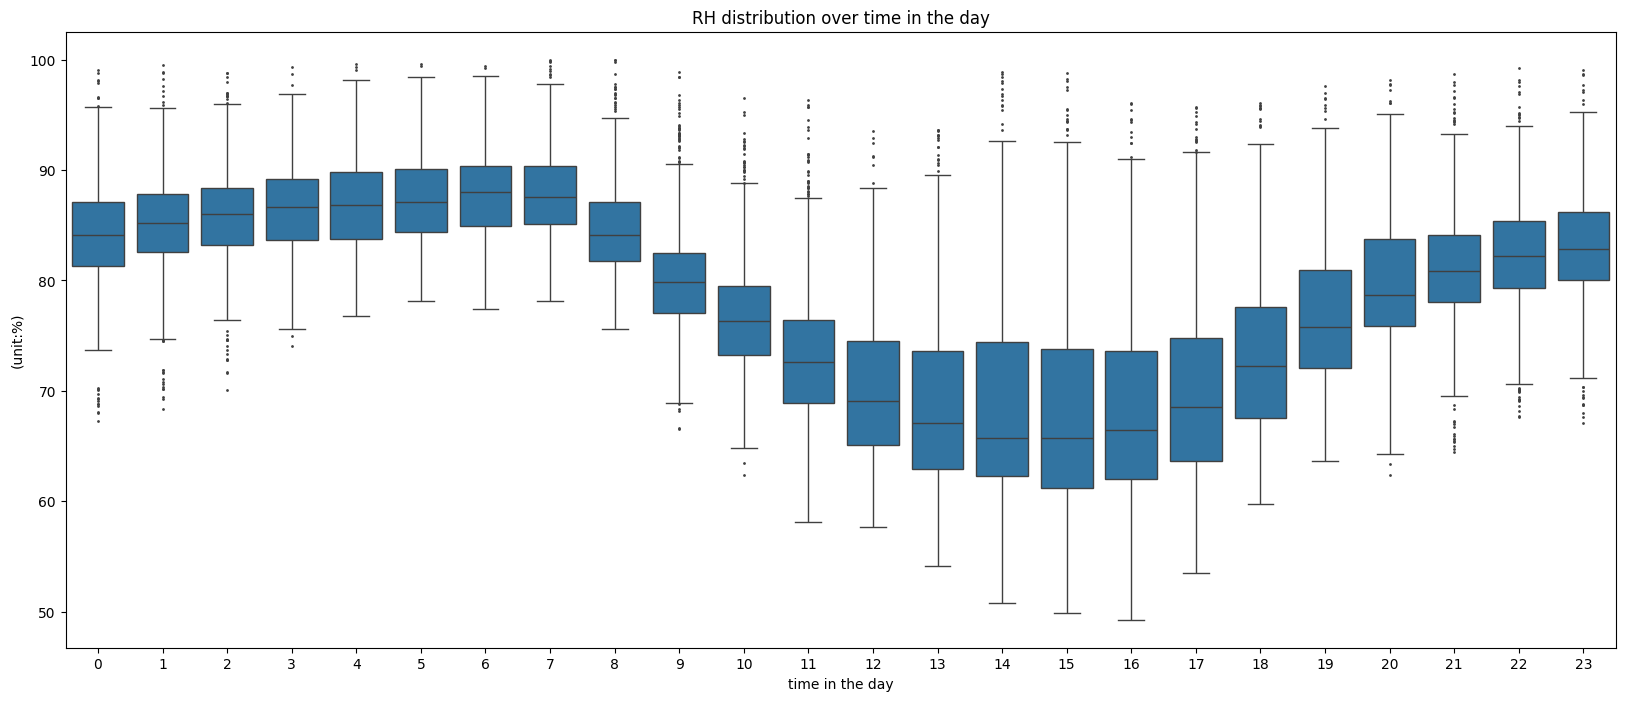
\includegraphics[scale=0.4]{figs/new_figs/rhboxplot.png}
 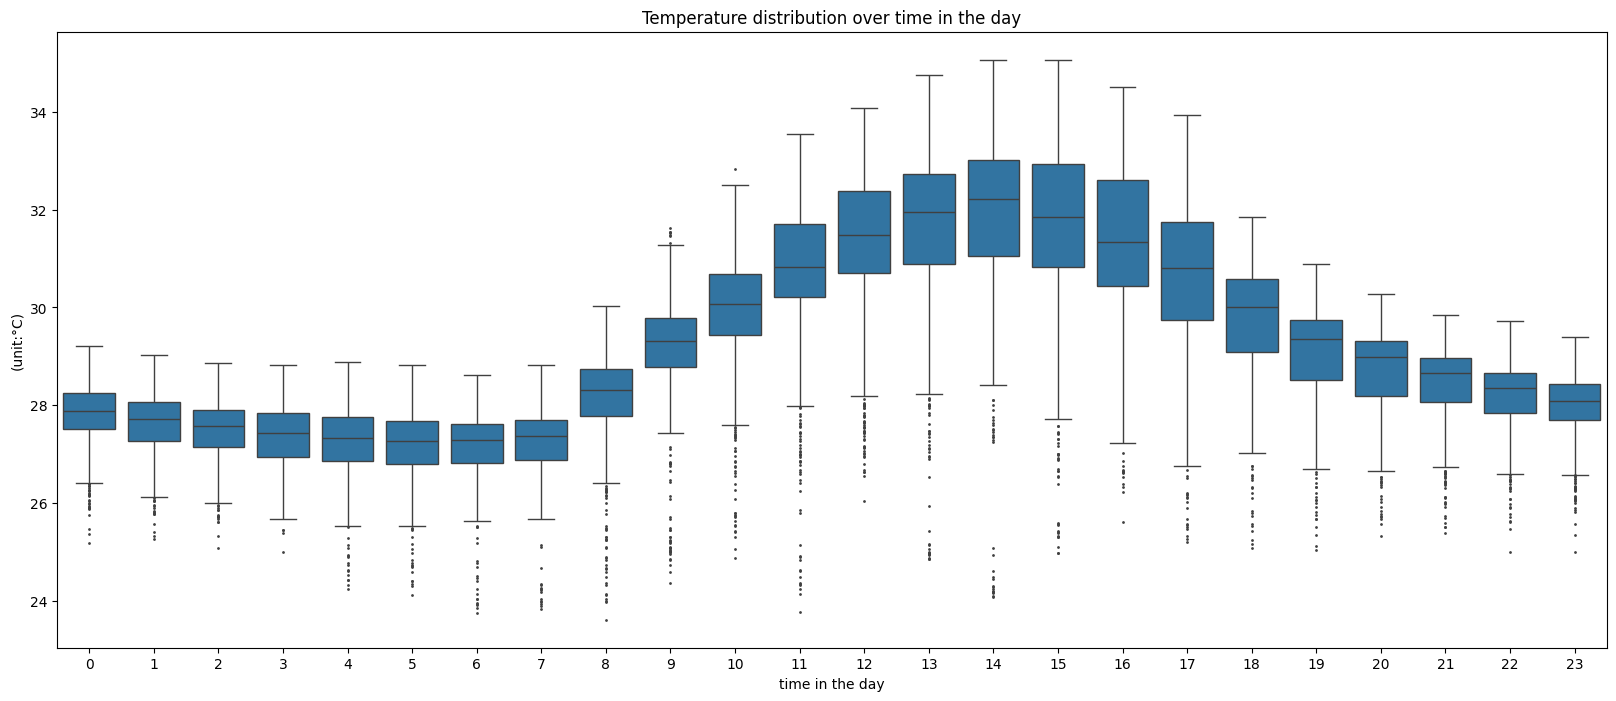
\includegraphics[scale=0.4]{figs/new_figs/temboxplot.png}
	\caption{The time series distribution of measures RH and Temperature.}
	\label{FIG:databoxplot}
\end{figure}


One month of data is deemed to be sufficient for this research because many of the climate variables in Singapore, such as temperature and relative humidity, do not show significant month-to-month variation. To illustrate this, we compute the Kullback–Leibler (KL) divergence (KL-divergence \citep{kullback1951information} is a statistical measurement from information theory that measures differences in information represented by two distributions.) between the distribution of one-month data and the entire year (Table \ref{KL divergence}). 


\begin{table}[width=.9\linewidth,cols=4,pos=h]
\caption{KL divergence. $P$ denotes the distribution over the whole year. $Q$ denotes the distribution of data collected in July 2019. $Q$ denotes the uniform distribution. $N$ denotes the normal distribution with the same mean and standard deviation as the whole year data.}\label{KL divergence}
\begin{tabular*}{\tblwidth}{@{} LLLLL@{} }
\toprule
Weather feature  & $KL(P||Q)$ & $KL(Q||P)$ &$KL(P||U)$&$KL(P||N)$\\
\midrule
RH &  0.1734 & 0.1443 & 0.4406&0.1571\\
Temperature& 0.1679&0.1489&0.3616&0.1280\\
\bottomrule
\end{tabular*}
\end{table}



When we attempt to fit a relatively complex distribution that we have observed with a simpler and common distribution (e.g.\ uniform distribution, binomial distribution), there may be a loss of information due to the discrepancy between the fitted distribution and the observed distribution. Kullback-Leibler (KL) divergence is introduced to measure the information loss and quantify the discrepancy between two probability distributions.  The formula of computing the $KL(P||Q)$ is shown as Equation~\ref{KL}. From Table~\ref{KL divergence}, it is evident from Table 2 that the $KL(P||N)$ is minimal, which shows that the data from July 2019 has a distribution similar to that of the whole year.

\begin{align}\label{KL}
    KL(P||Q)=\sum_{x}P(x)\log\left(\frac{P(x)}{Q(x)}\right)
\end{align} 

LULC classification is a systematic and complex study area. In traditional research, such data is often used for purposes like urban planning and construction over larger areas. The classification of LULC generally includes forests, farmlands (of different crops), lands, buildings, roads, water sources, and so on \citep{hutt2016best,vivekananda2021multi}. The classification of LULC can also be flexibly adjusted based on the research field and objectives \citep{gaur2023comprehensive}. In this small-scale microclimate study paper, considering the actual conditions of the research site, we primarily categorized LULC into the following types: distance to buildings, percentage covered by buildings, terrain (the height above sea level in meters), vegetated area, temporary area, urban canyon, distance to trees, distance to walkways, distance to roads, distance to paths, distance to court tracks, distance to car parks, percentage of road, percentage of paths, percentage of walkway, percentage of court tracks, percentage of car park, and number of trees. After applying a random forest regressor sensitivity analysis on a trial dataset, we select the 8 most important features, which are distance to buildings, distance to trees, distance to walkways, distance to roads, distance to paths, distance to court tracks, distance to car parks, and terrain. The values of the 8 features of LULC are derived from urban morphology data collected on the GIS map and buildings' 3D models of the NUS campus. The urban morphology data used in our study is in vector format, allowing us to choose an appropriate resolution based on our needs. The LULC data used in this study is collected on a grid of resolution of 1 m, ensuring high spatial density and providing more detailed geographical information.

\begin{figure}[!h]
	\centering
 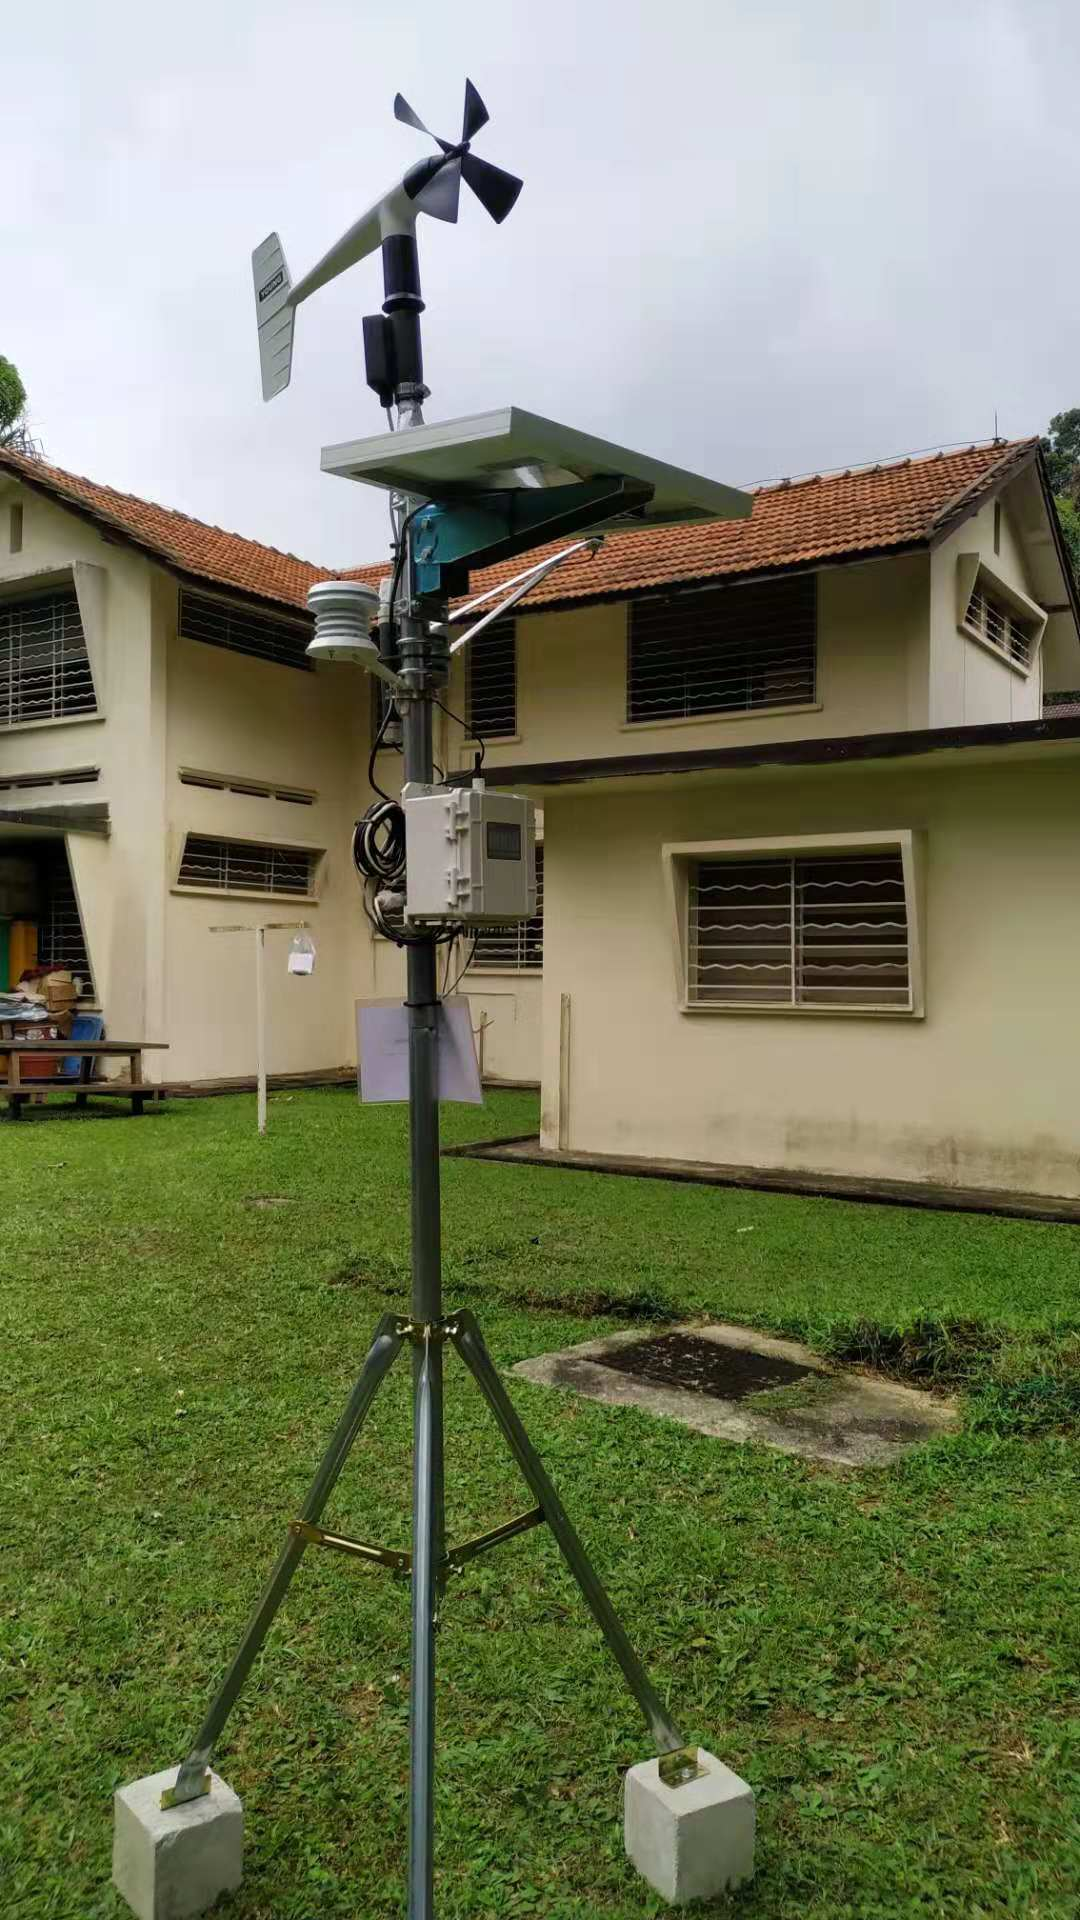
\includegraphics[height=5cm]{figs/new_figs/sensor_surrounding/12-3.jpg}
 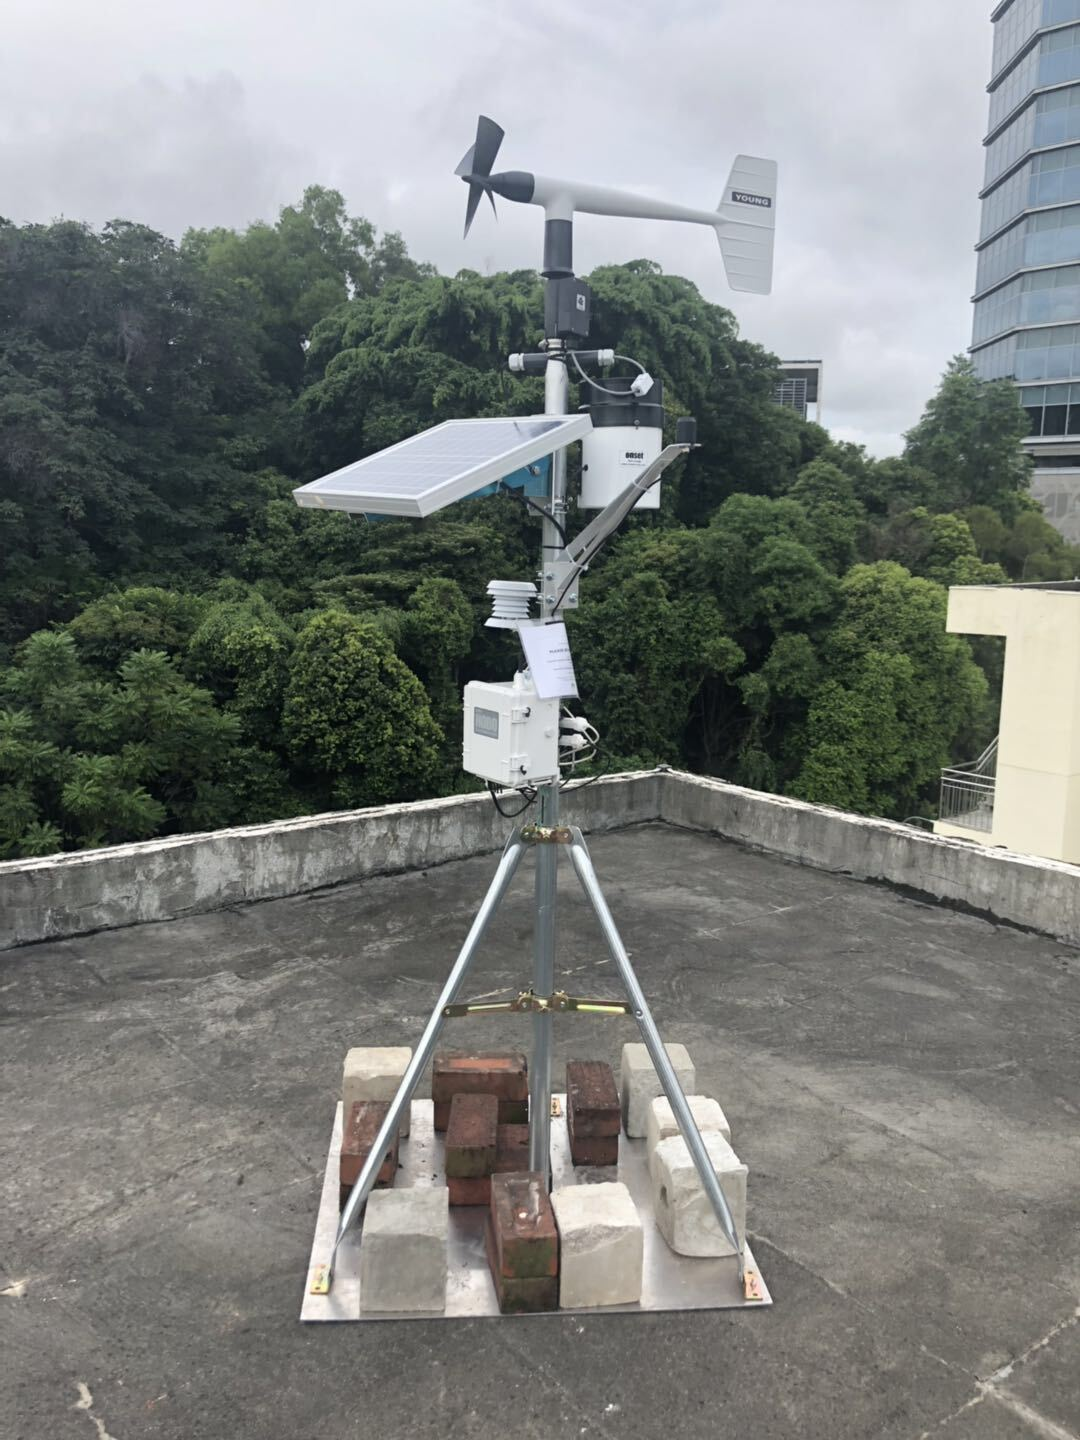
\includegraphics[height=5cm]{figs/new_figs/sensor_surrounding/14-2.jpg}
 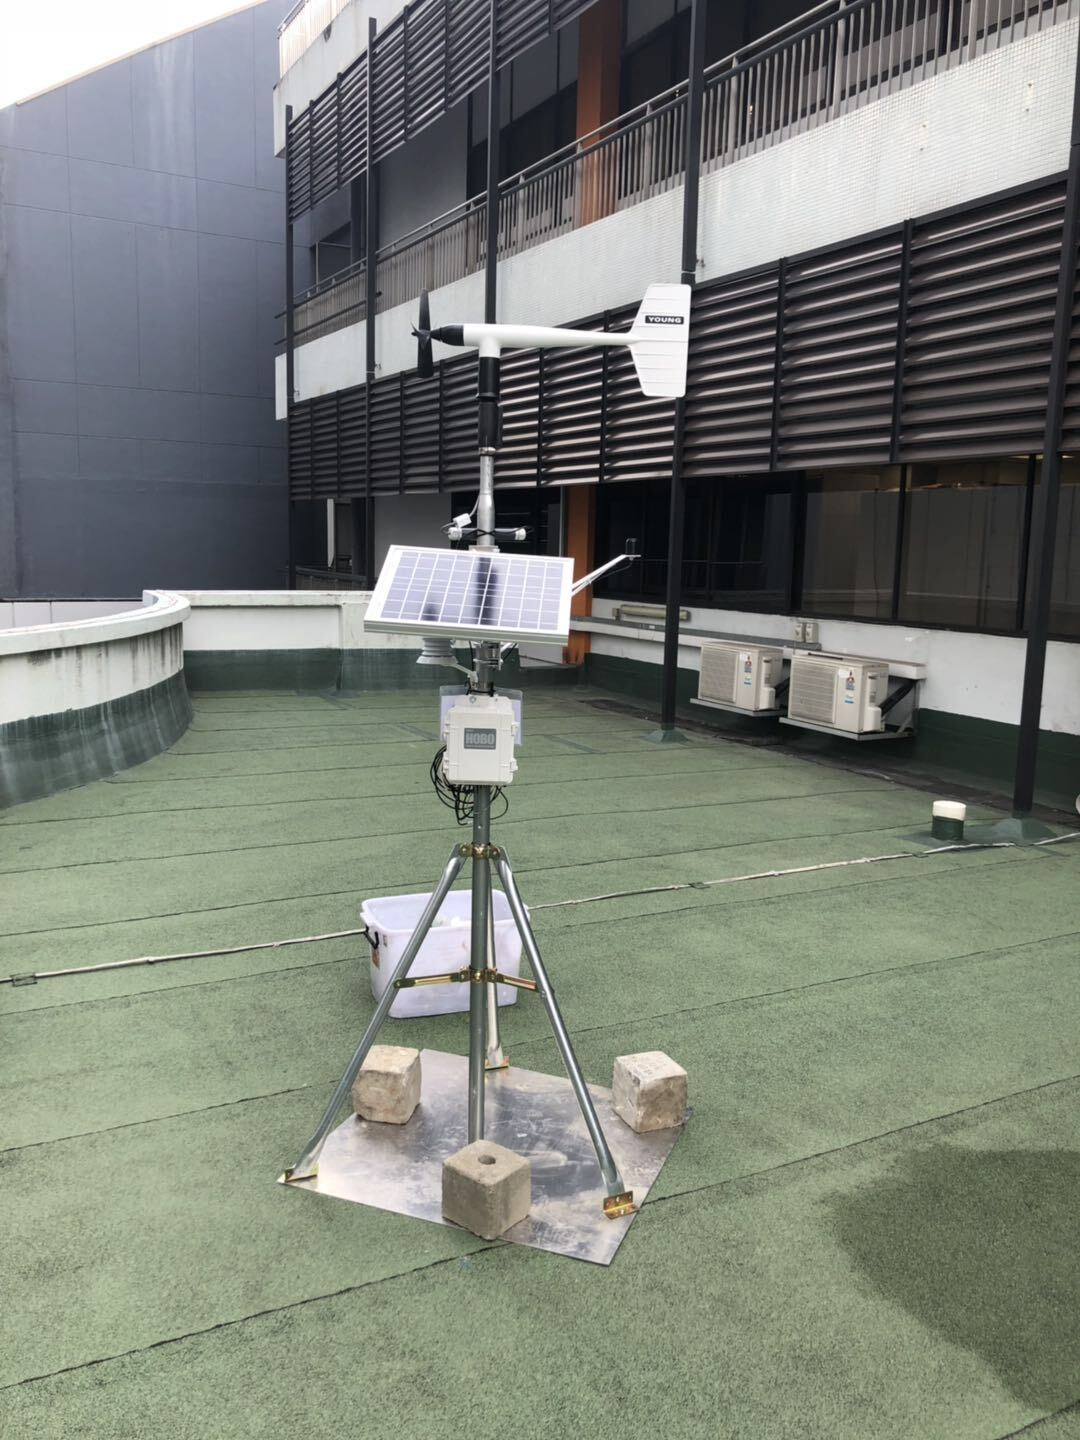
\includegraphics[height=5cm]{figs/new_figs/sensor_surrounding/15-2.jpg}
 \includegraphics[height=5cm]{figs/new_figs/sensor_surrounding/19-3.jpg}
	\caption{Example weather stations.}
	\label{fig:sensor}
\end{figure}

\subsection{Variable notations
}\label{ModelSetup}
Before delving into the detailed description of the model network structure, we will first introduce the relevant variables and their abbreviations in this section.

Given a time sequence of weather data after processing $\mathbf{X} = [x_1,x_2,\cdots,x_{T-1},x_T]$ with the time length $T$, where $x_t$ denotes the weather data information at time $t$. This model is to estimate the weather data at time $t$ of the target position $\mathbf{S^0}$, where $x_t\in \mathrm{R}^{N\times M}$ represents the observed value of $M$ weather features of $N$ weather stations, as shown in Equation (\ref{expression_x_t}).


\begin{equation}
    x_t=\left[
    \begin{matrix}
    x^{1,1}_t & x^{1,2}_t & \cdots & x^{1,M}_t\\
    x^{2,1}_t & x^{2,2}_t & \cdots & x^{2,M}_t\\
    \vdots & \vdots & \ddots & \vdots \\
    x^{N,1}_t & x^{N,2}_t & \cdots & x^{N,M}_t\\
    \end{matrix}\right]\label{expression_x_t}
\end{equation}
In the case here, there are 2 features, i.e. $M=2$. For convenience, we use $tem$ to denote the temperature and $rh$ to denote the relative humidity %, $vx$ and $vy$ to denote the wind speed of the west-east direction and north-south direction
respectively. 

To take the spatial information into concern, Equations (\ref{lat}) and (\ref{lng}) shows the coordinates of the stations in the local coordinate system.
\begin{flalign}
    \mathbf{s}&=[s^1,s^2,...,s^N]\label{lat}\\
    s^i&=[CoordX^i,CoordY^i]\label{lng}
\end{flalign}


The LULC data input is given for training use as the following Equation (\ref{LULC})
\begin{flalign}
    \mathbf{g}&=[g^1,g^2,\cdots,g^N]\label{LULC} 
\end{flalign}

%Here $g^i$ is a 5-dimensional vector that contains the ratio of terrain types of station $i$'s neighbor points. The five components are the ratio of road, path, walkway, court track, and car park respectively. $g^0$ is also an input of the model, which indicates the corresponding ratio around the target position. Other
Here $g^i$ is an 8-dimensional vector that contains the 8 LULC features used in the Regression Kriging model, these features are `terrain', `distance to building', `distance to tree', `distance to walkway', `distance to road', `distance to path', `distance to court track', and `distance to car park'. %Therefore 13 different LULC features in total are considered in this study. The LULC features used in the Regression Kriging model and their covariance matrix are shown in figure \ref{FIG:corr_LULC}.

\iffalse
\begin{figure}[!h]
	\centering
	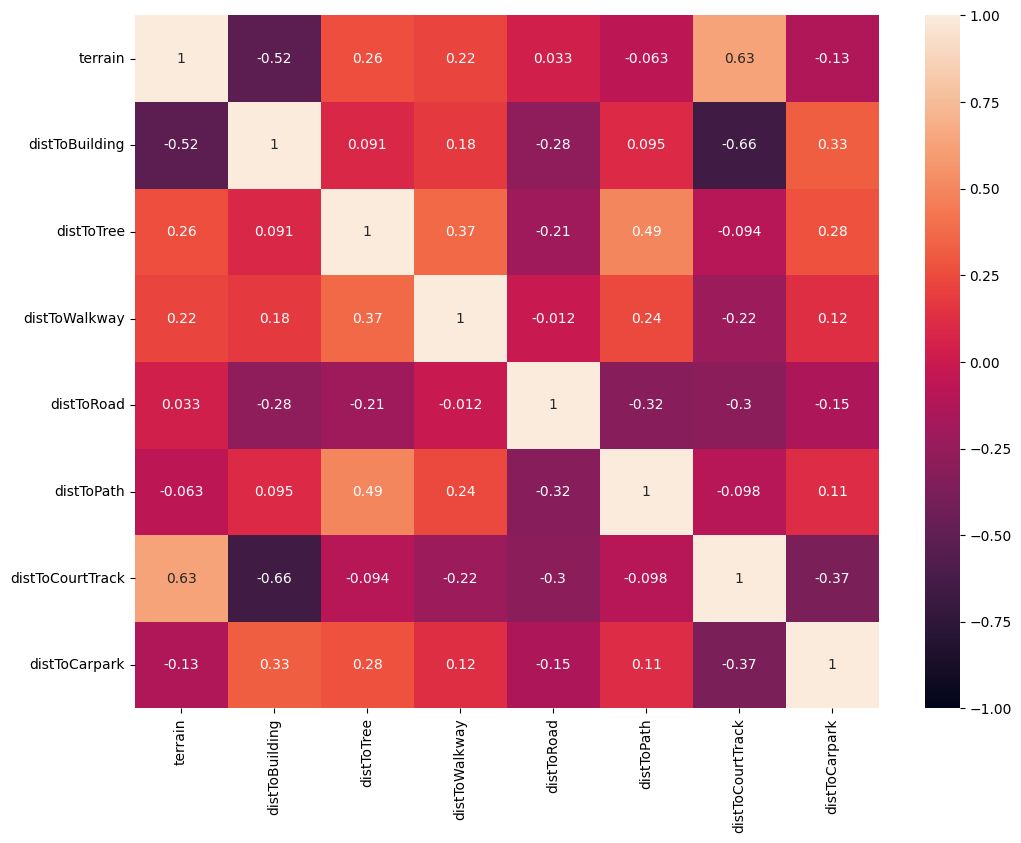
\includegraphics[scale=.45]{figs/new_figs/Correlationoffeatures.png}
	\caption{Correlation matrix of LULC features.}
	\label{FIG:corr_LULC}
\end{figure}
\fi

Combining the above equations, there are three parts of inputs in our model. Except for the LULC information $g^0$  we also need the target position $s^0=[CoordX^0,CoordY^0]$, and time series weather data of the stations, $[x_{t-r+1},x_{t-r+2},\cdots,x_{t}]$, where $t$ is the target time, $r$ is a hyperparameter representing the length of the time window. and our target output is $[tem^0_t,rh^0_t,vx^0_t,vy^0_t]$, which are the weather features of the target position.

\subsection{Model architecture design}\label{model_design}

The proposed model architecture is founded upon the fusion of using Long Short Term Memory (LSTM) to model temporal correlations and the Kriging model to model spatial correlation. 

The proposed network architecture comprises three primary components: the geographical layer, the Kriging layer, and the LSTM layer. The geographical layer integrates geographic information with observed station data, while the Kriging layer estimates time series data for the target location. The LSTM layer processes the temporal information of the time series data. The interconnections between the three layers are illustrated in Figure \ref{FIG:network}. 

\begin{figure}[!h]
	\centering
	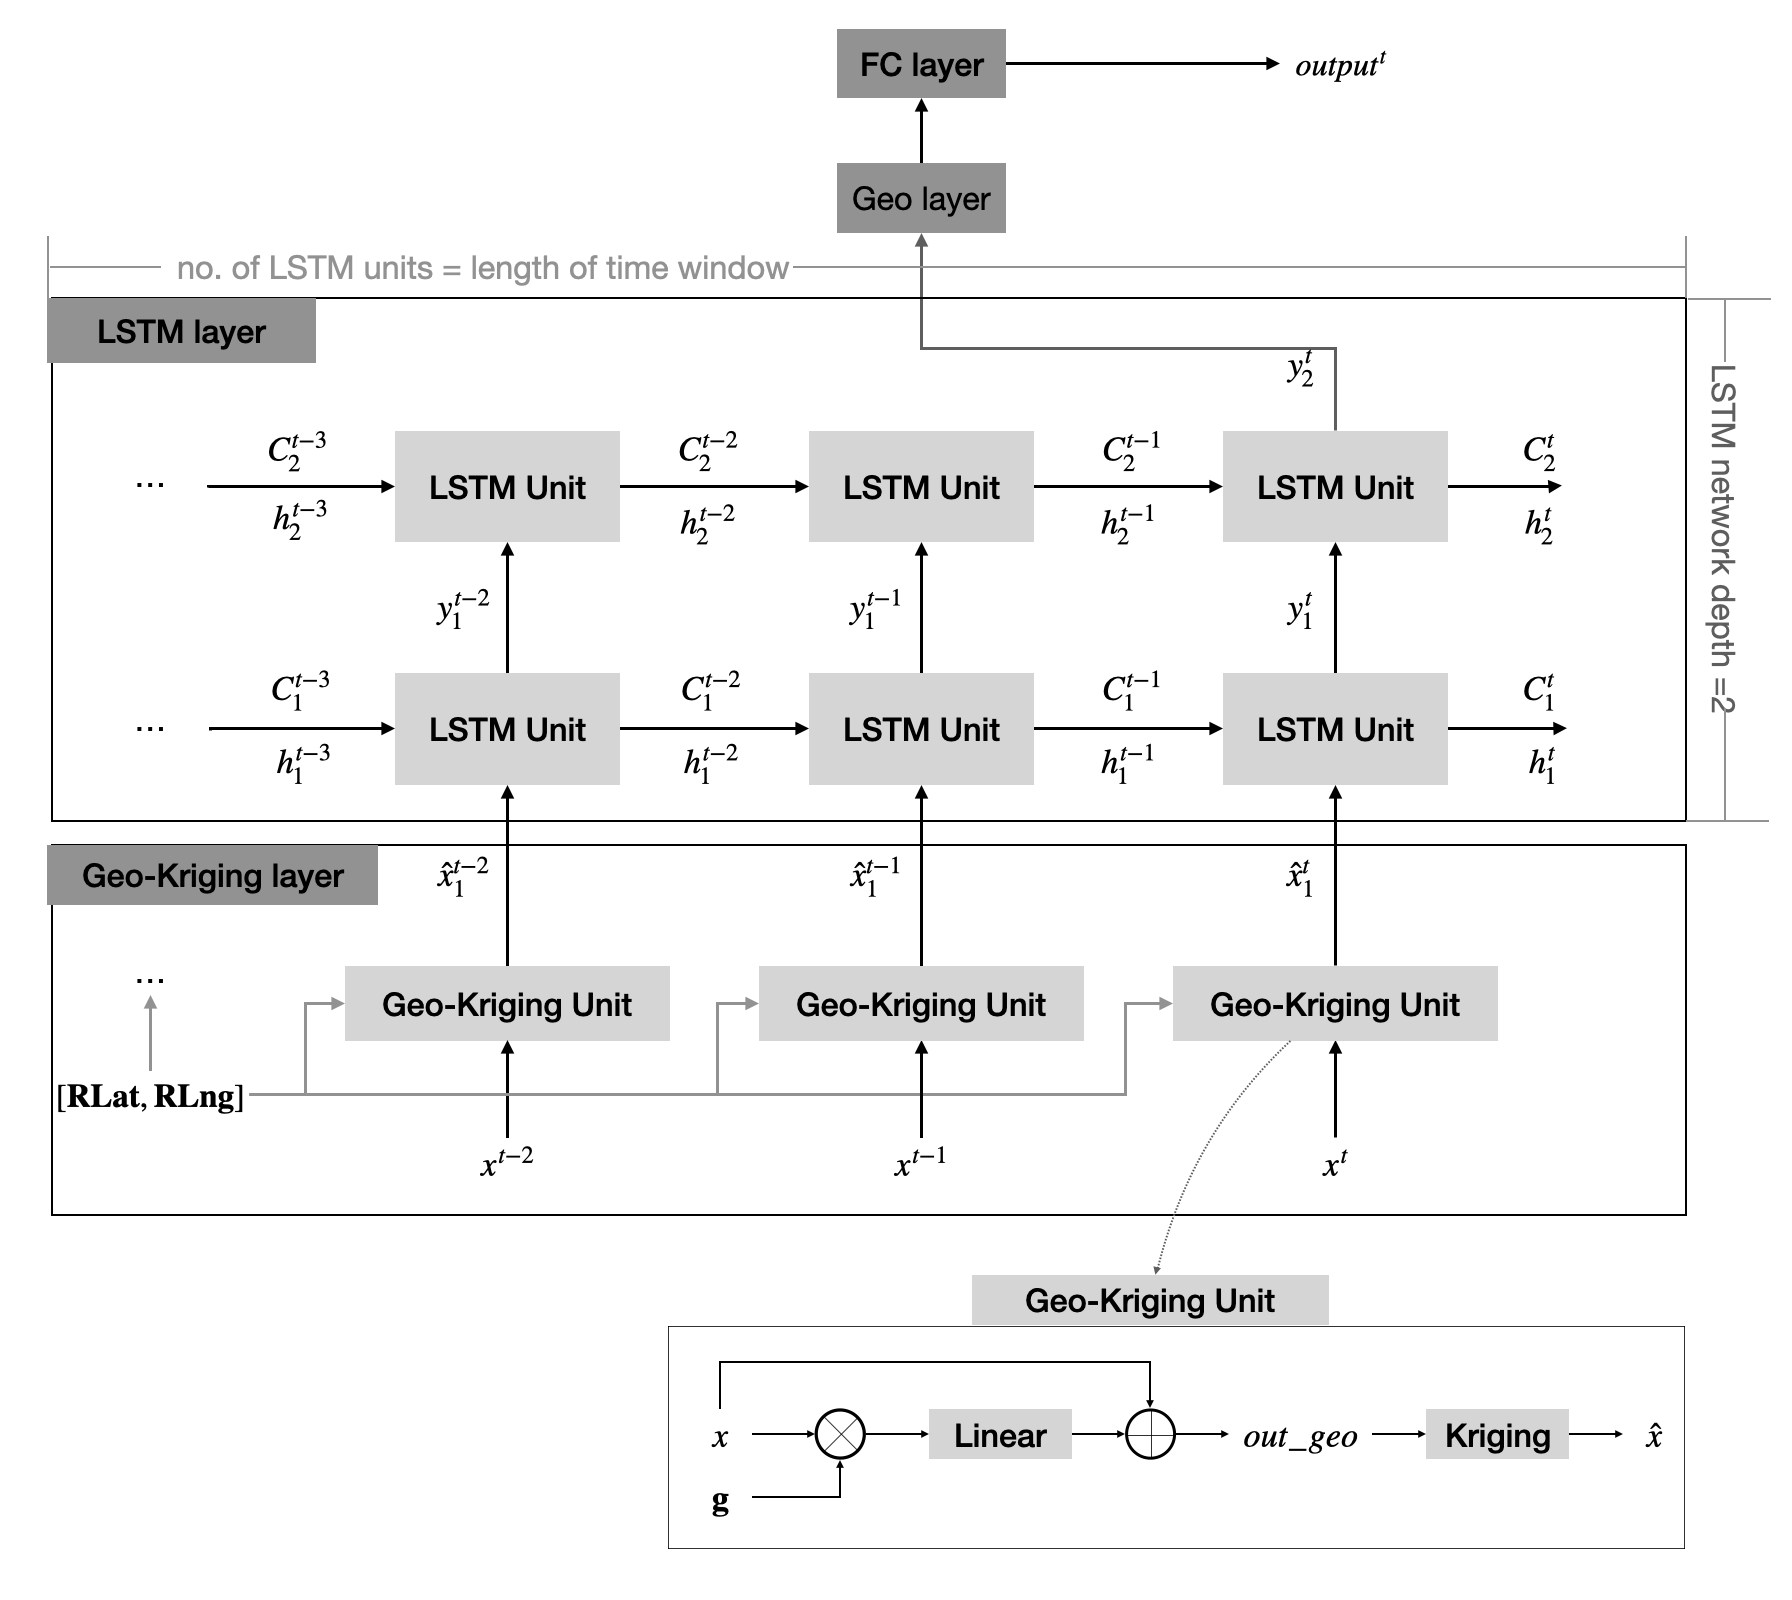
\includegraphics[scale=.5]{figs/network.png}
	\caption{Diagram of Geo-Kriging-LSTM network structure.}
	\label{FIG:network}
\end{figure}

\subsubsection{Geographical layer}
The geographical layers serve as filters to process the weather data. Specifically, the geographical layer takes the time series data $\mathbf{X}$ and geographic information $\mathbf{g}$ as inputs and employs a set of weights $\mathbf{c}=[c^1,c^2,\cdots,c^M]$ to modulate the weather features. When a weather station is located in a shaded area, its weather features are multiplied by the corresponding geographical weights ($\bold{g}$). 
%If the entire neighborhood of the station is not in shadow, then the weather features are left unchanged. When only a part of the neighborhood is in shadow, the output of the geographical layer is an interpolation between the two types of outputs. 
Specifically, the output of the geographical layer is given by the following formula:
\begin{flalign}
    out\_geo=\mathbf{X}*[\mathbf{g}\mathbf{c}^T+(1-\mathbf{g})\mathbf{1}^T]
\end{flalign}

where $\mathbf{1}=[1,1,\cdots,1]\in\mathbb{R}^{M\times 1}$
The output of the geographical layer is utilized as input data for the remaining part of the neural network. For the sake of notation simplicity, we will continue to use $X$ to refer to the output of the geographical layer. Since the input $\mathbf{g}$ represents the average value of the geographical information in the neighborhood, the geographical layer can be regarded as a layer similar to the convolutional layer.

\subsubsection{Regression Kriging layer}

In Section~\ref{ModelSetup}, a sensitivity analysis and screening were conducted on the available LULC data, resulting in the identification of 8 significant features. This subsection will elaborate on the detailed application of these features in the model.

The Regression Kriging layer generates the weather feature data in the whole computing area. At each time, the weather feature $x_t^0$ is interpolated by the weather station data predicted by the LSTM layer, $x_t^1,x_t^2,\cdots,x_t^M$. Using Regression Kriging, we have
\begin{flalign}
    x_t^0(s^0)=\sum_{i=1}^N \mathbf{w}^i \cdot q_i(s^0) + \sum_{i=1}^M \lambda^i \cdot e(s^i)
\end{flalign}
where $\mathbf{w}^i=[w^{i,1},w^{i,2},\cdots,w^{i,M}]^T\in \mathbb{R}^{1\times M}$ are the weights of the $i$th LULC feature, the first term denotes the deterministic part of the model. $\lambda^i$ are Kriging weights determined by the spatial dependence structure of the residual, and the second term interpolates the residual. 
These weights are the results generated from the Kriging layer.

In the Kriging method, we assume that the same type of weather data from all the weather stations has an identical distribution. And in order to estimate the weights we need to know the covariance between the weather data of two positions. Since LULC information has been considered in the geographical layer, a simpler model is used in the Kriging layer.
We assume that the covariance is only dependent on the distance between two positions. In equal, we use the following equality to estimate covariance:
\begin{flalign}
    Cov(x^{i,k}_t,x^{j,k}_t)=\gamma^k(d^{ij})\quad 1\leq i,j\leq N;\quad 1\leq k\leq M
\end{flalign}
where $\gamma^k$ (for $1\leq k\leq M$) are $M$ functions to estimate the covariance of variables, and $d^{ij}$ denotes the distance between station $i$ and station $j$. There are several parameters in each function, and the parameters in $\gamma^k$ will be learned in the network. In detail, we use the following ball correlation function: $\gamma^k$:
\begin{flalign}
    \gamma^k(d)=\begin{cases}
    b^k\left(1-\frac{3}{2}\frac{d}{a^k}+\frac{1}{2}\left(\frac{d}{a^k}\right)^3\right) & d\leq a^k\\
    0 & d>a^k
    \end{cases}
\end{flalign}
$a^k$ and $b^k$ are the parameters that represent the maximal correlation distance and variance of the type of weather data respectively.

Once the covariance is given, we can use the stochastic method to analyze that the optimal weights can be solved from the following linear equation system (\ref{eqn_Kriging_w}):
\begin{flalign}
    \left[
    \begin{matrix}
    \gamma^k(d^{11}) & \gamma^k(d^{12}) & \cdots & \gamma^k(d^{1N}) & 1\\
    \gamma^k(d^{21}) & \gamma^k(d^{22}) & \cdots & \gamma^k(d^{2N}) & 1\\
    \vdots & \vdots & \ddots & \vdots & \vdots \\
    \gamma^k(d^{N1}) & \gamma^k(d^{N2}) & \cdots & \gamma^k(d^{NN}) & 1\\
    1 & 1 & \cdots & 1 & 0\\
    \end{matrix}\right]\left[\begin{matrix}
    w^{1,k}\\
    w^{2,k}\\
    \vdots\\
    w^{N,k}\\
    \eta
    \end{matrix}\right]=\left[\begin{matrix}
    \gamma^k(d^{01})\\
    \gamma^k(d^{02})\\
    \vdots\\
    \gamma^k(d^{0N})\\
    0
    \end{matrix}\right]\label{eqn_Kriging_w}
\end{flalign}
$d^{0i}$ denotes the distance between target position and the station $i$, similar to the definition of $d^{ij}$. $\eta$ is a Lagrange parameter used as an intermediate variable. 

Once we know the value of Kriging weights, we can sum-product the weights and weather data together and get an estimation of the time series data for the target position. This time series data will be the input of the LSTM layer. The mechanism of the Geo-Kriging layer could be found in the logical diagram of Geo-Kriging unit in Figure \ref{FIG:network}.

\subsubsection{LSTM layer}

Long Short-term Memory (LSTM) \citep{hochreiter1997long} is derived from the Recurrent Neural Network (RNN), which can process sequential data. LSTM controls the transmission states by four gates to the memory of important knowledge and releases the memory of unimportant information, to achieve a balance of learning speed and accuracy for time series data prediction. It has been broadly applied in various areas including speed recognition, translation, prediction, etc. \citep{van2020review}. Built environment data is a representative time series kind of data, especially weather data, which is highly correlated with changes in the time of day. Therefore, the LSTM is a good basic model for the weather interpolation task. However, the existing methods combined with LSTM can only predict the features with historical data. The model proposed in this paper combines the strength of LSTM and Kriging interpolation, to calculate the weather features for the locations without historical data.

As shown in Fig. \ref{FIG:network}, the data processed by the Geo-layer and Kriging layer will continue to pass through the LSTM layer, where the historical knowledge could be memorized by each LSTM unit. Fig. \ref{FIG:Mechanism of each LSTM unit} shows the internal mechanism of each LSTM unit at time $t$. The hidden state of the last unit $h_{t-1}$, the cell state of the last unit $c_{t-1}$, together with the input data $x_t$ form the inputs of each LSTM unit, processed by four different gates in LSTM. The $f_t$ is the forgetting gate, represents the information of $C_{t-1}$ after oblivion to calculate $C_t$, the $C_t$ denotes the updated value of the unit state, calculated by the input data $x_t$ and the hidden state $h_{t-1}$. The $i_t$ is the input gate and the $o_t$ is the output gate. The final $o_T$ represents the output of the entire LSTM layer. In our model, T is set to 144, indicating the utilization of 24 hours of data for predicting data at 10-minute intervals within the next hour. These components work together to proceed to the LSTM layer. The detailed mathematical formula is listed in equations \ref{LSTM_gates}. 

\begin{figure}
	\centering
	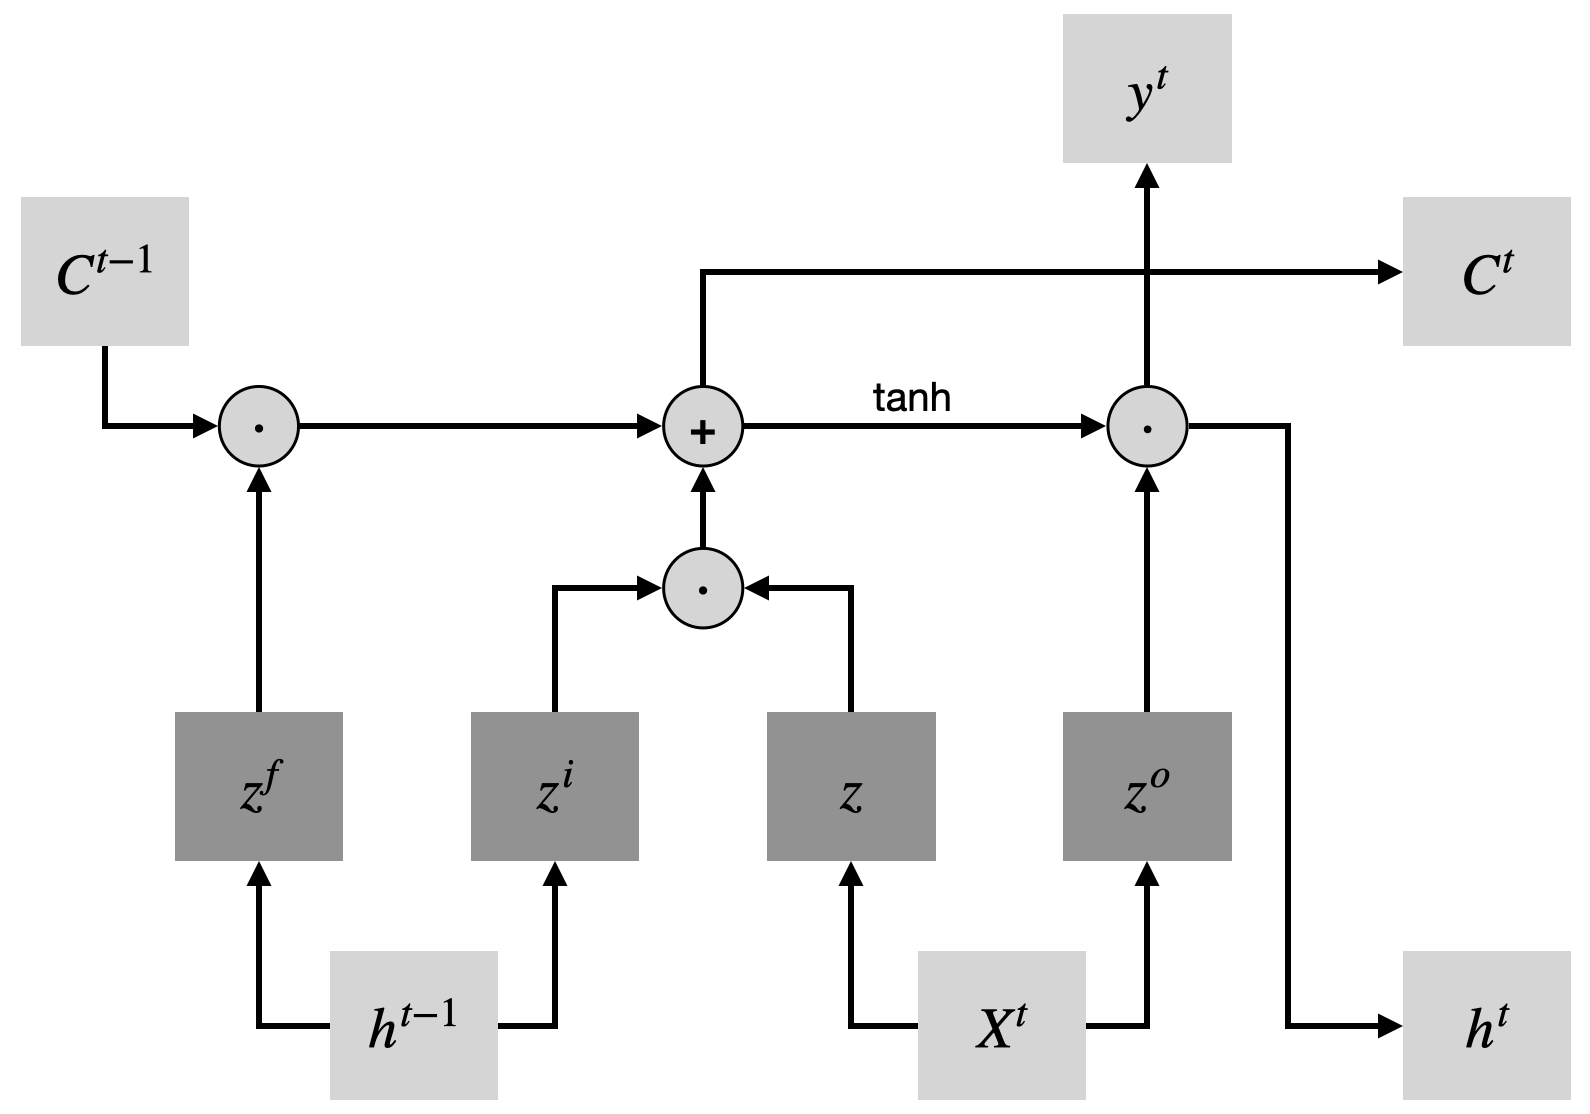
\includegraphics[scale=0.3]{figs/lstm_unit.png}
	\caption{Mechanism of each LSTM unit.}
	\label{FIG:Mechanism of each LSTM unit}
\end{figure}

\begin{flalign}
    f_t &= \sigma \ (W_f\cdot [h_{t-1},x_t]+b_f)\nonumber\\
    C_t &= f_t \times C_{t-1} +i_t\times \widetilde{C_t}\nonumber\\
    i_t &= \sigma \ (W_i\cdot[h_{t-1}, x_t]+b_C)\nonumber\\
    \widetilde{C_t} &= \tanh \ (W_C\cdot [h_{t-1},x_t]+b_C)\nonumber\\
    C_t &= f_t \times C_{t-1} +i_t \times \widetilde{C_t}\nonumber\\
    o_t &= \sigma \ (W_o \cdot [h_{t-1},x_t]+b_o)\nonumber\\
    h_t &= o_t \times \tanh \ (C_t)
    \label{LSTM_gates}
\end{flalign}



%As mentioned in section \ref{Related Work}, traditional microclimate prediction methods include conventional interpolation techniques, machine learning methods, and direct utilization of data from nearby weather stations or urban weather files. Therefore, the experimental design of this study consists of two main parts. Firstly, the various methods mentioned above will be used as baselines to compare the performance of the proposed model. Secondly, based on the feasibility of the model, the study will explore the integration of LULC data and attempt to reduce the reliance on weather station data. This aims to investigate whether satisfactory prediction results can still be achieved with fewer computational resources. The results of the above experiments will be discussed in detail in the next section.

\subsection{Clustering methods for time series data}

As the predicted results are all time series data, for a comprehensive analysis of time series results later in the text, common time series classification methods were employed in this study. There are many existing methods. \cite{abanda2019review} broadly categorized into three types: feature-based, model-based, and distance-based methods. Complex classification methods are suitable for higher-dimensional time series data. Therefore, for the task of classifying time series data in this paper, we adopted the classic dynamic Time Warping (DTW) algorithm. It is widely appreciated for its efficiency in measuring similarity between time series, effectively mitigating the impacts of time shifts and distortions. It achieves this by enabling a flexible transformation of time series, allowing the detection of similar shapes even with different phases \citep{senin2008dynamic}. 

Simultaneously, for the purpose of correlating the complex temporal classification results with their diverse features, we employed the 
Principal Component Analysis (PCA) \citep{mackiewicz1993principal} to reduce the dimensionality of the data. This method is commonly used in handling high-dimensional large datasets, as it can reduce data dimensionality, thereby enhancing data interpretability while minimizing information loss \citep{jolliffe2016principal}. Similarly, in this paper, we applied a similar approach to the high-dimensional temporal classification results, aiding us in analyzing the impact of various LULC features on prediction results.
\subsubsection{Dynamic Time Warping (DTW)}\label{DTW}
In general, DTW is a method that calculates an optimal match between two given time series with certain restrictions and rules:

Every index from the first sequence must be matched with one or more indices from the other sequence, and vice versa
The first index from the first sequence must be matched with the first index from the other sequence (but it does not have to be its only match)
The last index from the first sequence must be matched with the last index from the other sequence (but it does not have to be its only match)
The mapping of the indices from the first sequence to indices from the other sequence must be monotonically increasing, and vice versa. We can plot each match between the sequences $1:M$ and $1:N$ as a path in a $M\times N$ matrix from $(1,1)$ to $(M, N)$, such that each step is one of $(1,0),(0,1),(1,1)$. In this formulation, we see that the number of possible matches is the Delannoy number.

The optimal match is the match that satisfies all the restrictions and the rules and that has the minimal cost, where the cost is computed as the sum of absolute differences, for each matched pair of indices, between their values.

The sequences are "warped" non-linearly in the time dimension to determine a measure of their similarity independent of certain non-linear variations in the time dimension. This sequence alignment method is often used in time series classification. 

\subsubsection{ Principal Component Analysis (PCA)}\label{PCA}
PCA can be thought of as fitting a p-dimensional ellipsoid to the data, where each axis of the ellipsoid represents a principal component. For a column-wise zero empirical mean data matrix $\bold{X}$, the first component weight vector $w_{(1)}$ maximizes the data variance, so it must satisfies:
\begin{equation}
    w_{(1)}=\text{arg}\max_{||w||=1}\left\{ \sum_{i}(x_{(i)}\cdot w)^2\right\}=\text{arg}\max_{w}\left\{ \frac{w^\intercal\bold{X}^\intercal\bold{X} w}{w^\intercal w}\right\}
\end{equation}
other weight vectors can be obtained by continuing this progress after subtracting $\bold{X}ww^\intercal$ from $\bold{X}$. For example,
\begin{equation}
    w_{(2)}=\text{arg}\max_{w}\left\{ \frac{w^\intercal\bold{X_{(1)}}^\intercal\bold{X_{(1)}} w}{w^\intercal w}\right\},\quad \text{where} \bold{X_{(1)}}=\bold{X}-\bold{X}w_{(1)}w_{(1)}^\intercal
\end{equation}
the component of $\bold{X}$ on $w_{(i)}$ direction is the $i$th principle component of $\bold{X}$, which is called $p[i]$ in Figure \ref{FIG:station8tem} we will show in the later sections.

\section{Results}\label{Results}

As indicated in Section \ref{Methodology}, the weather data utilized in the experiments were sourced from weather stations and LULC data of the study area. To evaluate the performance of our model against existing microclimate prediction methods, we conducted a comparative study. When evaluating the model performance, considering that the target locations for prediction do not have weather stations, the historical weather data for the current prediction location is unavailable. To simulate such practical situation, it is crucial to avoid the direct inclusion of historical weather data for the target locations in the input dataset. Therefore, we adopted the commonly used method of cross-validation in machine learning: when predicting the weather data for each weather station, we excluded its own historical weather data and utilized only the historical weather data from other weather stations.

\subsection{Evaluation Approach}\label{evaluation method}

In order to evaluate the model performance, the subsequent analysis of the results involves two types of baselines and commonly used error metrics. This section provides a detailed description of them.

\subsubsection{Baselines}\label{baselines}

In existing studies, researchers often use urban weather files data or data from representative weather stations near the research target to access microclimate data for multiple types of studies. Therefore, to comprehensively validate the actual performance of the model proposed in this paper, we designed two levels of baselines. These baselines are compared with the experimental results of the model from the perspectives of machine learning algorithms and practical application scenarios. Our baselines consist of the following: 
\begin{itemize}
\item Comparing the model with classical types of machine learning models to select the optimal algorithm that combines spatial and temporal data. These are the level 1 baselines. The selected temporal baselines include LSTM and GRU, which are representative algorithms to process historical data; the selected spatial baselines include Ordinary Kriging and Regression Kriging interpolation.
\item Comparing the experimental results of the optimal ML algorithm with traditional microclimate data accessing methods, including directly using data from neighboring weather stations, representative urban weather stations (Weather station in Changi Airport), and International Weather for Energy Calculations (IWEC) data. The comparison could demonstrate the accuracy of our microclimate prediction method, also showing the practical implications.

\end{itemize}

In order to conduct these studies, we compare the performance of the proposed Geo-LSTM-Kriging model.


%Therefore, the baselines used in this study are summarized in table \ref{baseline table}.
%\begin{table}[width=0.6\linewidth,cols=2,pos=h]
%\caption{Baselines of 2 levels.}\label{baseline table}
%\begin{tabular*}{\tblwidth}{@{} LL@{} }
%\toprule
%Level 1 &\begin{tabular}[c]{@{}ll}Temporal methods & Spatial methods \\\midrule LSTM & Linear interpolation\\ GRU & IDW interpolation\\ & Kriging interpolation\\ \end{tabular}\\
%\midrule
%Level 2 &\begin{tabular}[c]{@{}l}
    %Data of the nearest weather station on the NUS campus  \\
    %Data of urban weather station data at Changi Airport\\
%\end{tabular}\\
%\bottomrule
%\end{tabular*}
%\end{table}

\subsubsection{Metrics}\label{metrics}

Mean Square Error (MSE), Rooted Mean Square Error (RMSE), and R-Squared are computed as evaluation metrics. Equations (\ref{eqn_metrics}) show the definition of these metrics. The error plotted in this paper is $e_i$ in the equations. %Normalized Mean Square Error (NMSE), Mean Absolute Error (MAE), Mean Relative Error (MRE),  
\begin{flalign}
    O_i&:\text{observed values,  }S_i:\text{simulated values} \quad e_i=S_i-O_i:\text{error}\nonumber\\
    \text{MSE}&=\frac{1}{N}\sum_{i=1}^N({e_i})^2=\frac{1}{N}\sum_{i=1}^N({O_i-S_i})^2\nonumber\\
    \text{RMSE}&=\sqrt{\text{MSE}}=\sqrt{\frac{1}{N}\sum_{i=1}^N({O_i-S_i})^2}\nonumber\\
    %\text{NMSE}&=\frac{\text{MSE}}{\frac{1}{N}\sum_{i=1}^N{O_i}^2}\nonumber\\
    %\text{MAE}&=\frac{1}{N}\sum_{i=1}^N|e_i|=\sum_i|O_i-S_i|\nonumber\\
    %\text{MRE}&=\frac{\text{MAE}}{\frac{1}{N}\sum_{i=1}^N|O_i|}\nonumber\\
    R^2&=1-\frac{\sum_{i=1}^N({O_i-S_i})^2}{\sum_{i=1}^N(O_i-\bar{O})^2}
    \label{eqn_metrics}
\end{flalign}

\subsection{Baseline comparison}

In this section, we will elaborate on the comparison between the model proposed in this paper and the two-level baselines mentioned in Section~\ref{baselines}. We can discover the spatial and temporal trends of the local microclimate, as well as identify the environmental factors that influence the microclimate through the comparison of these experimental results.

\subsubsection{Comparison with ML baselines}

Due to the temporal nature of microclimates, in this paper, we conducted an hourly statistical analysis of the prediction results for all the weather stations, as shown in Figure \ref{FIG:baselines1}. The horizontal axis represents the sequential time from 0 to 24 hours each day, while the vertical axis represents the absolute error between predicted values and actual values. The upper chart represents humidity, and the lower chart represents temperature. The box plots in the figure illustrate the trends of errors for each day and at each weather station location. The different colors represent the following different models: the Geo-LSTM-Kriging model, LSTM-Kriging model, GRU-Kriging model, Kriging model, and the IDW model respectively. It can be observed that for the humidity prediction results, we can see that traditional interpolation methods exhibit significant fluctuation in model prediction errors during the daytime from 11 a.m. to 6 p.m. In contrast, machine learning models reduce this error fluctuation, maintaining stable prediction errors throughout. However, both the LSTM-K and GRU-K machine learning models show a larger range of error fluctuations from around 0 a.m. to 8 a.m. Our GEO-LSTM-K model, on the other hand, maintains stable performance throughout the entire 24 hours. On the other hand, concerning the temperature prediction results, various methods show higher errors and greater variability during the daytime from 10 a.m. to 6 p.m. 

For the fluctuation of prediction errors, it is evident that one reason is the significant variability in actual observational data during the corresponding time intervals, as depicted in Figure \ref{FIG:databoxplot}. The characteristics of this raw data naturally influence the prediction results, and a larger range of data fluctuations increases the difficulty of prediction, thereby introducing greater variance in prediction errors. However, at the same time, we can observe that machine learning methods, especially the Geo-LSTM-Kriging model incorporating the geo layer, outperform traditional interpolation models significantly (RMSE of Geo-LSTM-Kriging reduces from 1.602 / 0.701 to 0.637 compared to IDW / LSTM-Kriging respectively, shown in Table \ref{tab:RMSE}). This indicates that machine learning, along with the introduction of the geo layer, contributes to the model capturing new knowledge. This kind of fluctuation is reasonable in urban meteorology, as various factors such as local natural conditions like solar radiation, shading, rainfall, the surrounding built environment related to UHI effect, urban heat exchange, and more contribute to increased instability in meteorological data during the day. 

To further analyze the optimization effect and explore what knowledge the models have acquired by Geo-layer, we summarize the variance and data fluctuation range of these two models in Figure \ref{FIG:baselines3}. This figure contrasts the Geo-LSTM-Kriging and LSTM-Kriging models extracted separately from the previous figure. Differing from Figure \ref{FIG:databoxplot}, the blue numbers in this figure represent the standard deviation of the prediction errors for the Geo-LSTM-Kriging model during each hour, while the orange numbers represent the standard deviation for the LSTM-Kriging model. Upon closer inspection, it can be observed that during periods of significant fluctuations in the original data (refer to Figure \ref{FIG:databoxplot}, specifically the early morning humidity and afternoon temperature periods), the addition of the Geo-layer results in more stable predictions, with a noticeably larger reduction in variance. For example, the standard deviation of temperature prediction errors decreased from 0.96 to 0.57 at 13:00 in the afternoon, while it only decreased from 0.67 to 0.41 at 23:00 at night. The overall statistical results (RMSE) and R-square be summarized after comparing with the level-2 baselines, as shown in Table \ref{tab:RMSE}. 

This suggests that the geo layer, to some extent, has learned the varying impact of environmental factors such as UHI on temperature and humidity during different time periods. Our model aims to uncover the underlying reasons for how geographical environmental factors influence the performance of meteorological data, thereby providing more stable predictive results. In the above figure, we have depicted the model prediction errors at all weather stations locations in boxes. Apart from time series analysis, different LULC features among various weather stations can also have varying effects on prediction performance. Detailed analysis of how these LULC features specifically affect model performance will be presented in the subsequent spatial analysis, after the comparison with level-2 baselines



\begin{figure}[!h]
	\centering
        	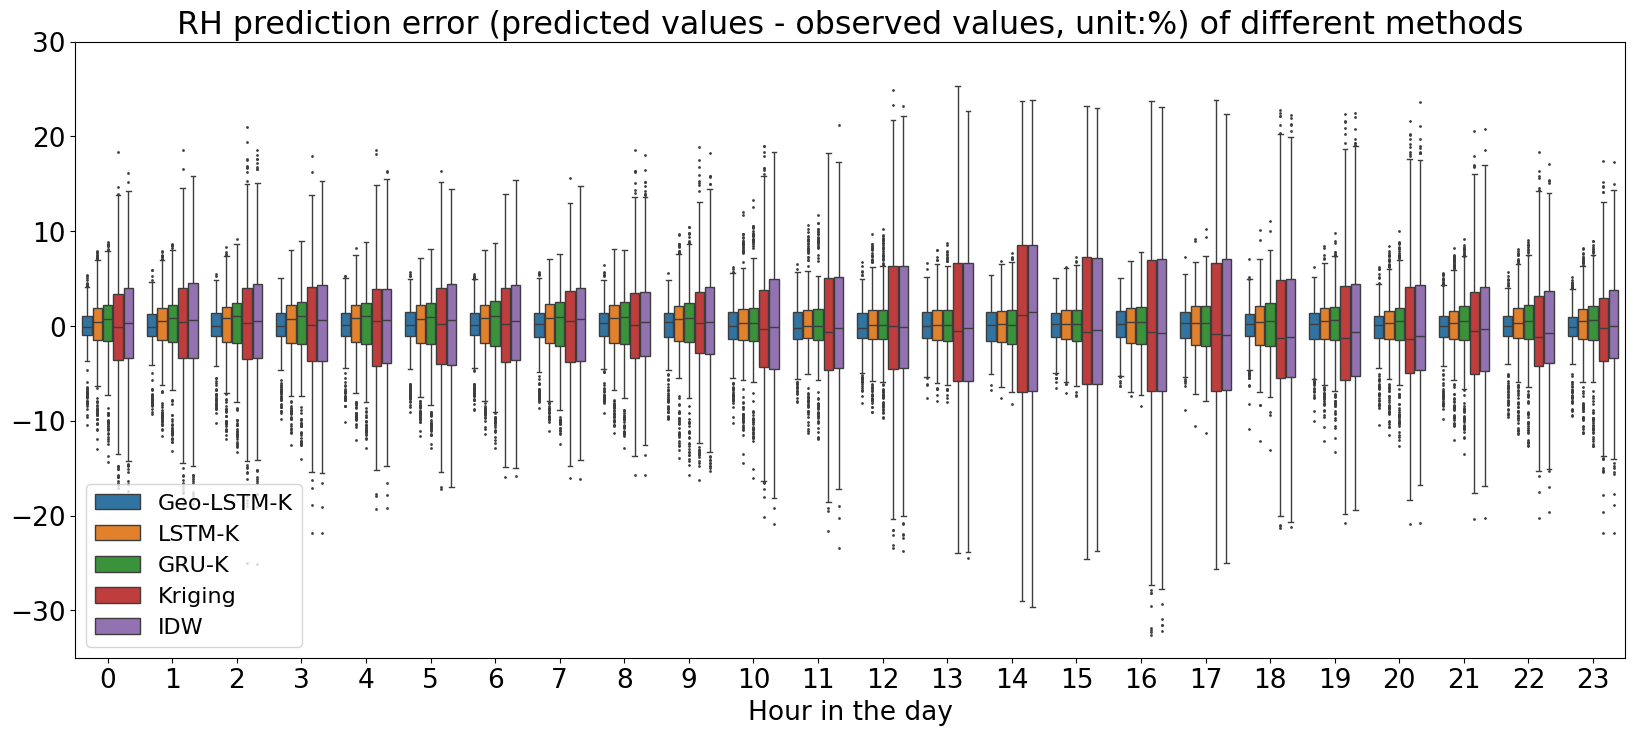
\includegraphics[scale=0.38]{figs/new_figs/RH5models.png}
	    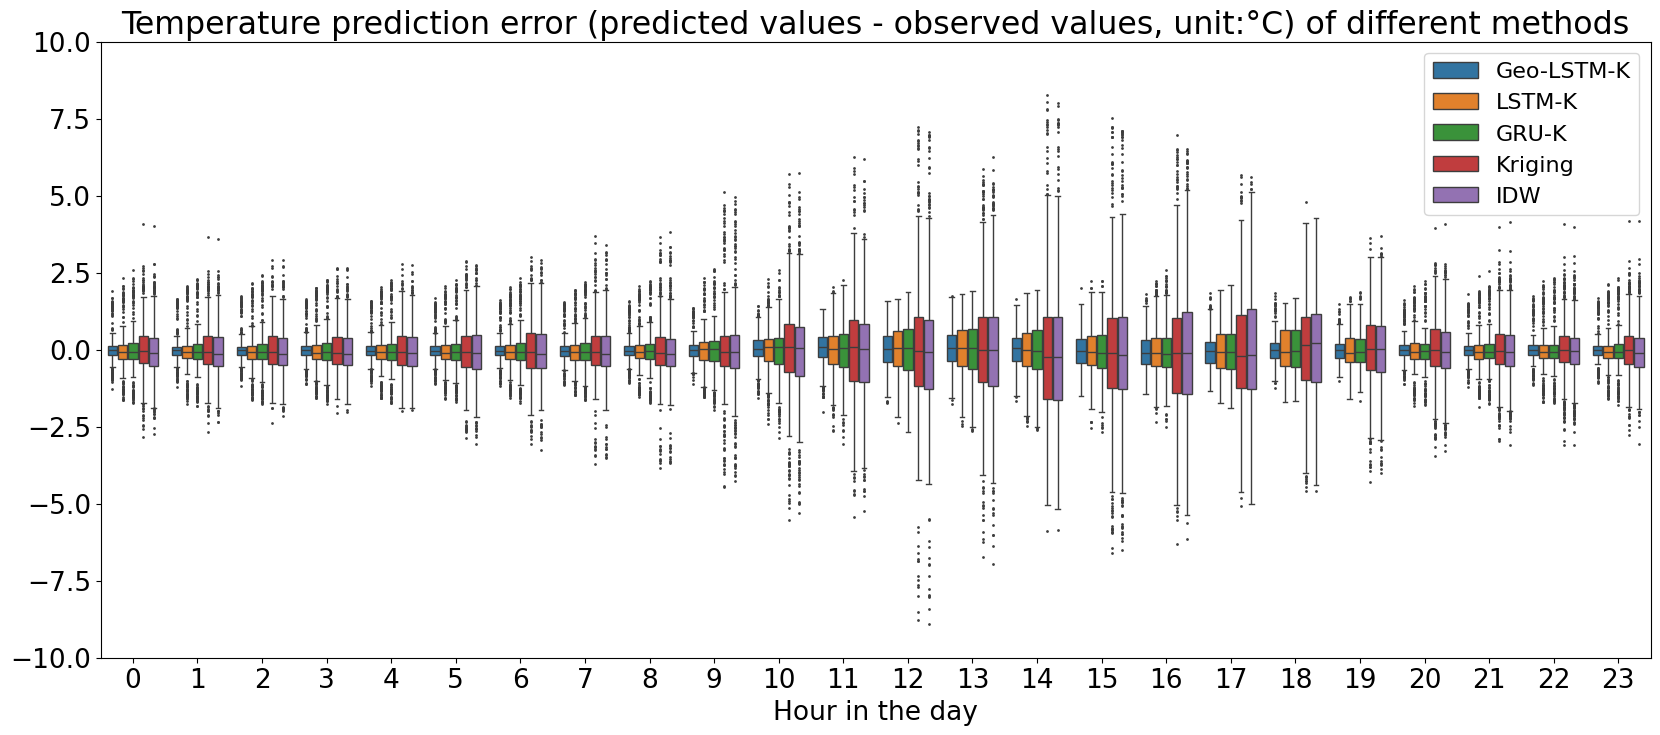
\includegraphics[scale=0.38]{figs/new_figs/Tem5models.png}
	\caption{Temporal comparison between LSTM-Kriging and ML (level 1) baselines.}
	\label{FIG:baselines1}
\end{figure}

\begin{figure}[!h]
	\centering
	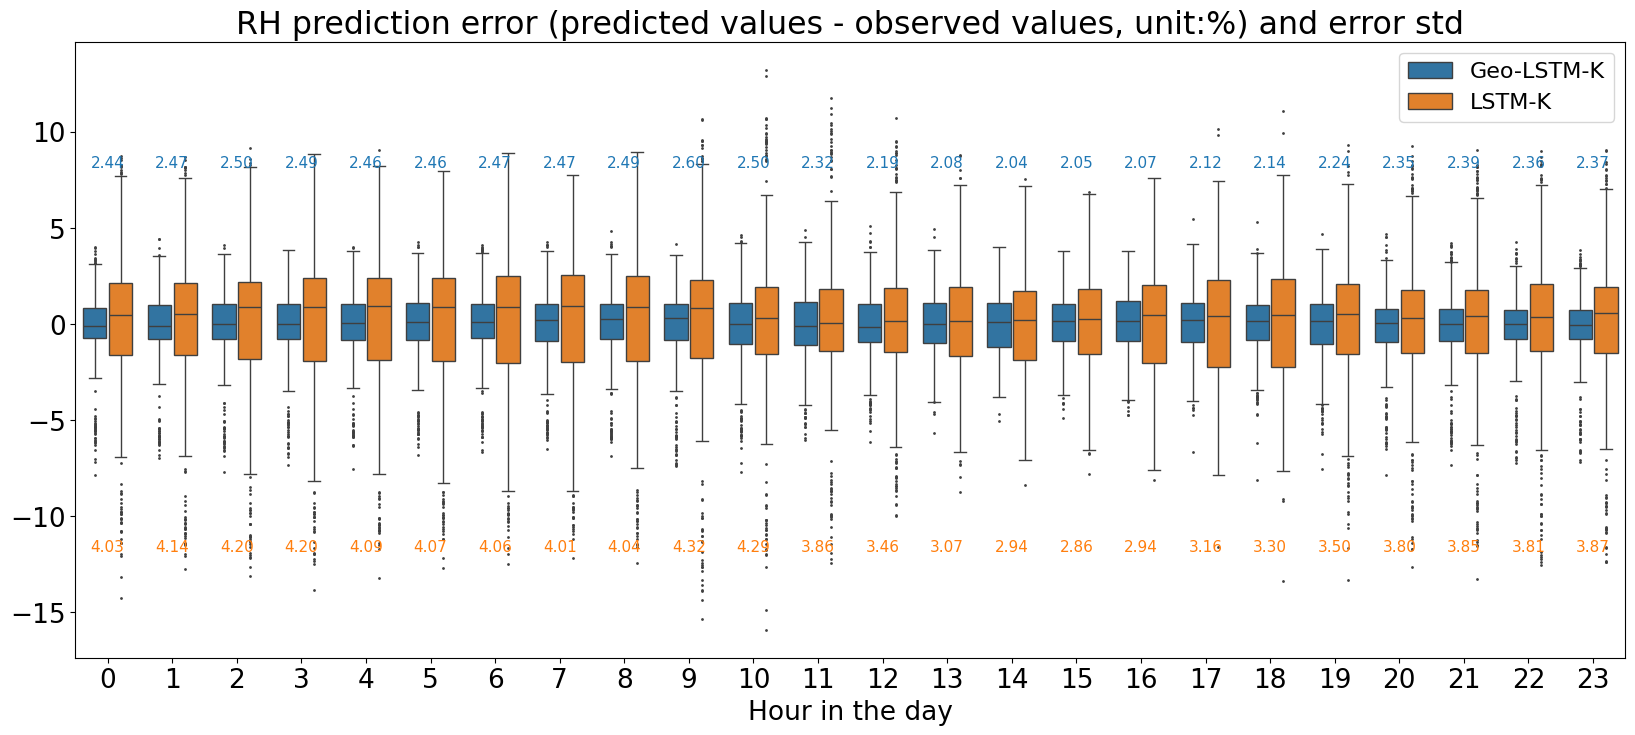
\includegraphics[scale=0.29]{figs/new_figs/RHerrstd.png}
    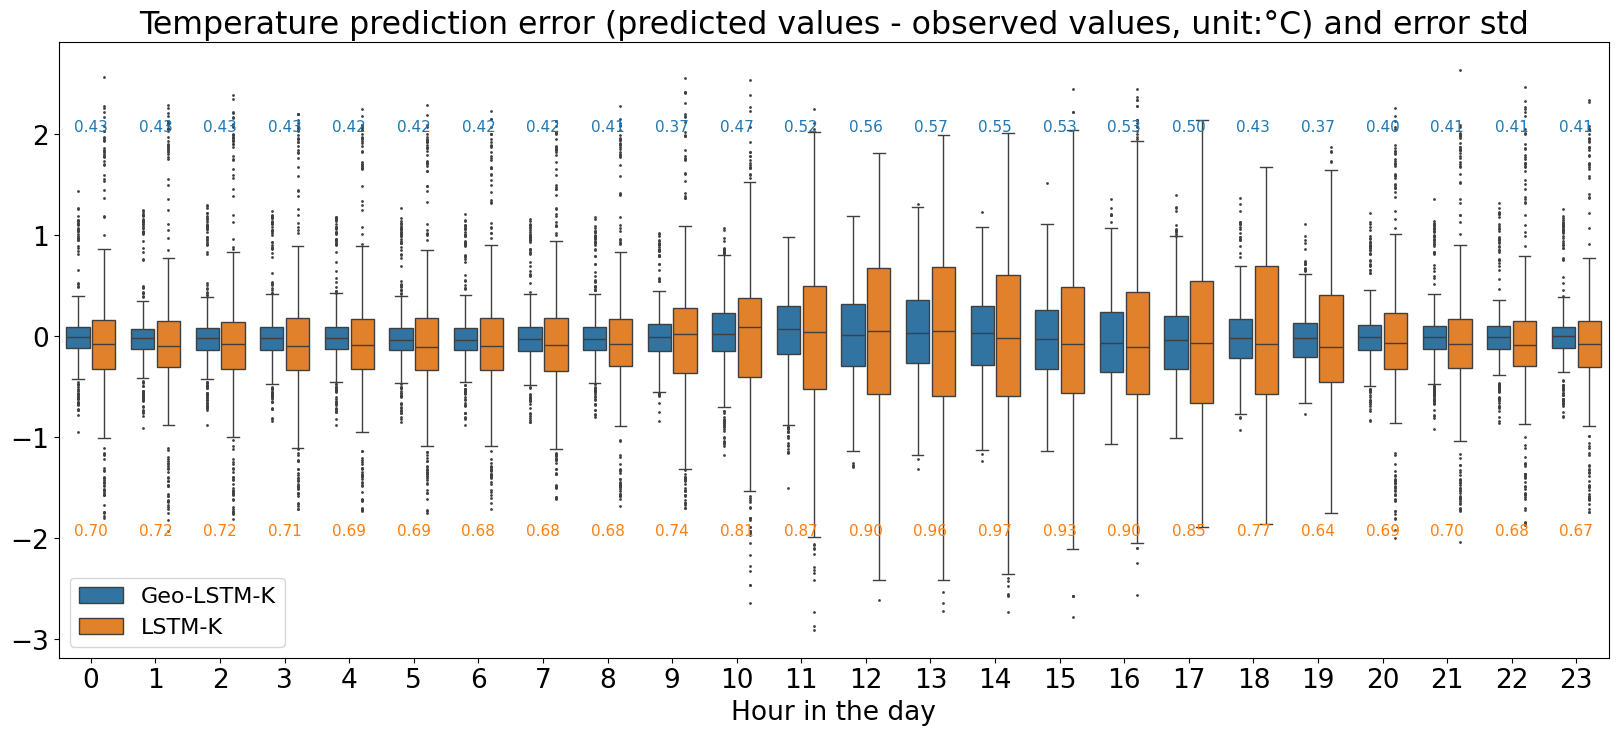
\includegraphics[scale=0.29]{figs/new_figs/temerrstd.png}
	\caption{Temporal comparison between Geo-LSTM-Kriging and LSTM-Kriging.}
	\label{FIG:baselines3}
\end{figure}



%The comparison results with level 1 baselines are shown in Figure \ref{FIG:baselines}. We can observe that comparing with other machine learning models, LSTM-Kriging demonstrated the lowest error. The MSE reduction of temperature from 1.48\%(0.44\textdegree C) to 0.82\%(0.24\textdegree C) (improved by 44.59\%), RH from 0.86\%(0.82) to 0.60\%(0.57) (improved by 30.23\%), by replacing the linear layer with the Kriging layer. And compared with the IDW method, LSTM-Kriging reduces the MRE of temperature from 2.09\%(0.62\textdegree C) to 0.82\%(0.24\textdegree C) (improved by 60.77\%), and the MRE of RH from 1.33\%(1.26) to 0.60\%(0.57) (improved by 54.89\%). Therefore, we employed LSTM-Kriging as the core model and attempted to further enhance its performance by incorporating LULC data, which is detailed in the subsequent section

%We can observe that when compared with other machine learning models, LSTM-Kriging exhibited the lowest error. The MAE on the test set of the LSTM-Kriging is lesser than the baselines by about 0.2$^o$C, while that of RH is lesser than the baselines by about 0.69. From the respective magnitudes of temperature and humidity (the average temperature for the entire month is 28.0°C, and the average RH is 83.2\%), it can be observed that the prediction error for humidity is relatively smaller. This result is acceptable and explainable, as it can be reasonably inferred that humidity fluctuates less over a larger spatial range, unlike temperature which is affected by factors such as sunlight, shading, and wind. As the LSTM-Kriging has a better prediction of microclimate parameters, we use it as the core model and attempt to enhance its performance further using LULC data, as described in the subsequent section.

%The MAE reduction of temperature from 0.44\textdegree C to 0.24\textdegree C, RH from 0.82 to 0.57, by replacing the linear layer with the Kriging layer. Compared with the IDW method, LSTM-Kriging reduces the MAE of temperature from 0.62\textdegree C to 0.24\textdegree C, and the MAE of RH from 1.26 to 0.57. Therefore, we employed LSTM-Kriging as the core model and attempted to further enhance its performance by incorporating LULC data, which is detailed in the subsequent section.

%After adding Geo-layer to the LSTM-Kriging model, the average MAE across all stations of temperature reduces from 0.24\textdegree C to 0.12\textdegree C, of RH reduces from 0.57 to 0.39. 

%To further verify the effectiveness of the Geo-LSTM-Kriging model, we further proceed with the following several experiments to see the time series performances in detail. 

%We observe the model performance on each station separately using LSTM-Kriging and Geo-LSTM-Kriging. We conclude that for all 14 stations, the Geo-LSTM-Kriging model always has a lower error than the LSTM-Kriging model for temperature prediction continuously. Meanwhile, the presence of the Geo-layer contributes to more stable predictions, where the variance of the predictions with the geo-layer is consistently lower across all weather stations. This indicates that the introduction of LULC data has allowed the model to learn environmental information to some extent, making the calculation and control of prediction results more stable.

\iffalse
\begin{table}[width=.9\linewidth,cols=4,pos=h]
\caption{Overall comparison of Geo-LSTM-Kriging and LSTM-Kriging.}\label{Overall comparison of geo}
\begin{tabular*}{\tblwidth}{@{} LLLLLL@{} }
\toprule
Model and predicting weather feature  &MSE & NMSE & MAE & MRE & $R^2$\\
\midrule
Geo-LSTM-Kriging temperature& 1.3268 & 0.0126& 0.1210 & 0.41\% & 0.9372\\
LSTM-Kriging temperature & 
2.5937 & 0.0257 &0.2424 & 0.82\%&0.8938\\
Geo-LSTM-Kriging RH& 2.7351 & 0.1045& 0.3977 & 0.41\% & 0.9596\\
LSTM-Kriging RH & 
3.6241 & 0.1367 &0.5820 & 0.60\%&0.9103\\
\bottomrule
\end{tabular*}
\end{table}
\fi

%To be more detailed in temporal dimension, the Geo-LSTM-Kriging model demonstrates higher prediction accuracy compared to the LSTM-Kriging model during the afternoon. We conclude three typical types of stations based on the model performance, whose land use properties are shown in Figure \ref{FIG: LULCdata}. The prediction results of these stations are presented in Figure \ref{FIG:TIMEanalysis_example}. It shows that the majority of improvements in temperature occur between 12:00 and 15:00, suggesting that the incorporation of geographical information allows the Geo-LSTM-Kriging model to capture the distribution of weather features more effectively under strong sunlight or rapidly changing conditions since a higher variance is observed. The incorporation of Geo-layer provides the maximum improvement by reducing the average MAE across all stations of temperature from 0.61\textdegree C to 0.12\textdegree C, of RH from 2.06 to 0.53, compared to the LSTM-Kriging model. Conversely, there is limited enhancement observed during the night. We summarize the experiment result data in Table \ref{Overall model analysis}.

\iffalse
\begin{figure}[!h]
	\centering
	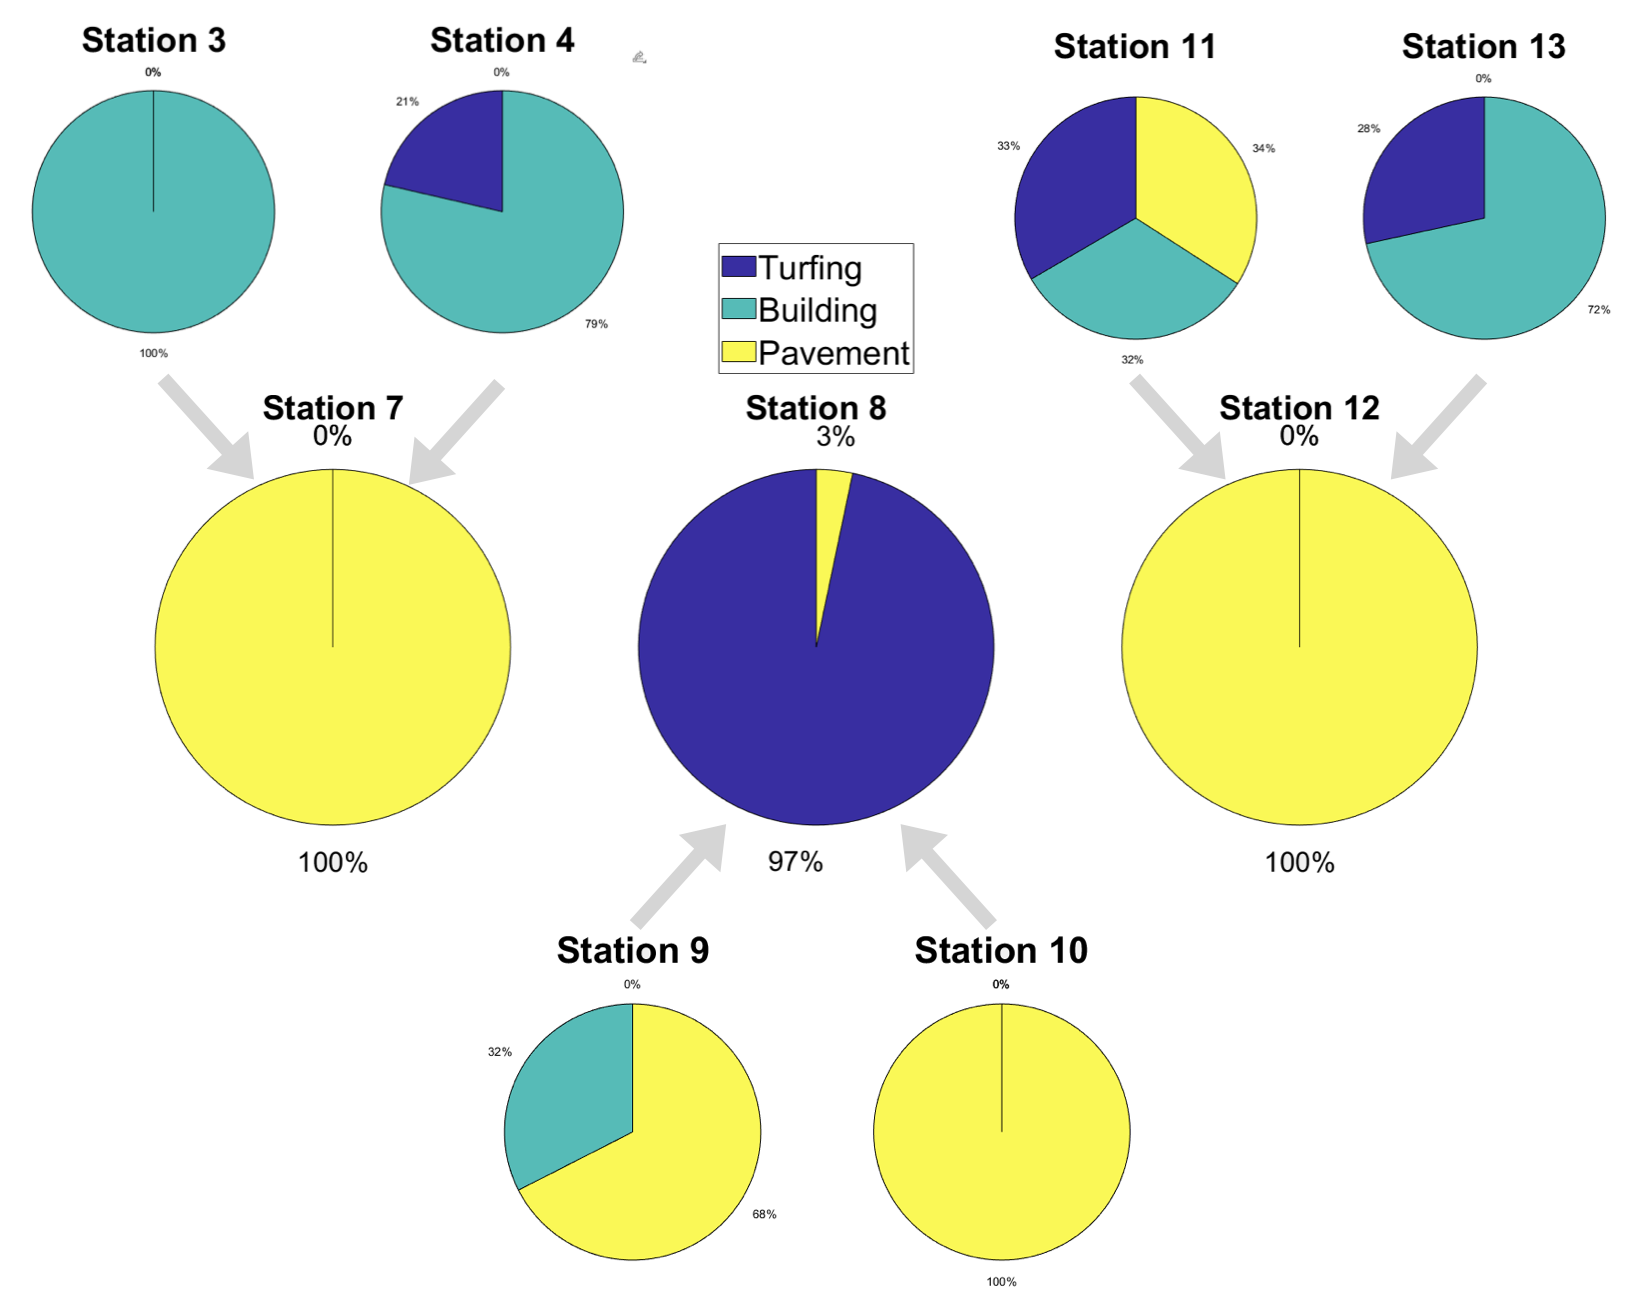
\includegraphics[scale=0.45]{LULCdata.png}
	\caption{LULC data of 3 typical stations and their two neighboring stations.}
	\label{FIG: LULCdata}
\end{figure}
\begin{figure}[!h]
	\centering
	\includegraphics[scale=0.55]{figs/timeseries_example.png}
	\caption{MAE with the standard deviation of MAE at stations. Stations 7, 8, and 12 are shown as examples. The horizontal axis denotes the time of the day, the mean is taken over one hour.}
	\label{FIG:TIMEanalysis_example}
\end{figure}
\fi

\iffalse
\begin{table}[width=1.0\linewidth,cols=5,pos=h]
\caption{Analysis of solar radiation effect on temperature prediction.}\label{Overall model analysis}
\begin{tabular*}{\tblwidth}{@{} LLLLL@{} }
\toprule
Criteria &  Object & Metrics &Parameters & Comments\\
\midrule
%Best point & Station 4 & $R^2_T$:0.7734 $R_{RH}^2$:0.9176& Shown in Fig.\ref{FIG:map2} & \begin{tabular}[c]{@{}l}More accurate at \\the denser stations\end{tabular}\\
%Worst point & Station 8 & $R^2_T$:0.5959 $R^2_{RH}$:0.7514& Shown in Fig.\ref{FIG:map2}& \begin{tabular}[c]{@{}l}Less accurate at \\the isolated stations\end{tabular}\\
Best time period &0:00-6:00 &$R^2_T$:0.9587-0.9438&\begin{tabular}[c]{@{}l}
     Average solar radiation:  \\
     $1.07W/m^2$ 
\end{tabular} &\begin{tabular}[c]{@{}l}More accurate when\\ the sunlight is weak\end{tabular}%, and temperature changing speed is slow
\\
Worst time period & 12:00-15:00 &  $R^2_T$:0.8795-0.8539&\begin{tabular}[c]{@{}l}
     Average solar radiation:  \\
     $336.08W/m^2$ 
\end{tabular}
& \begin{tabular}[c]{@{}l}Less accurate when \\the sunlight is strong \end{tabular}\\
Best improvement period & 12:00-15:00 & MRE improvement: 80.61\% &\begin{tabular}[c]{@{}l}
     Average solar radiation:  \\
     $336.08W/m^2$ 
\end{tabular} & \begin{tabular}[c]{@{}l}Improvements are obvious \\when the sunlight is strong\end{tabular}\\  
\bottomrule
\end{tabular*}
\end{table}
\fi


%As for the spatial analysis, the three trends shown in Figure \ref{FIG:TIMEanalysis_example} correspond to the three stations described in Figure \ref{FIG: LULCdata}. Upon observation, it can be noticed that Stations 7 and 12 have similar LULC conditions, both having a green coverage ratio of 0. These stations exhibit a trend in the figure where the errors are larger during periods of high solar radiation intensity. However, Station 7 performs worse than Station 12. We speculate that it is due to the presence of neighboring stations (3 and 4) with higher green coverage ratios and significant geographical variations. While Station 8 has a higher green coverage ratio, the model mitigates its errors during periods of high solar radiation intensity. However, since there are no neighboring stations with similar high green coverage ratios, the overall error level for Station 8 remains higher. Therefore, the different prediction performance is reasonable, as locations with similar geographical environments often exhibit similar microclimate characteristics. We will discuss this matter in more detail in Section \ref{Discussion}.

\iffalse
\begin{table}[width=.9\linewidth,cols=4,pos=h]
\caption{LULC data of the three typical stations.}\label{LULC data of 3 stations}
\begin{tabular*}{\tblwidth}{@{} LLLLLLLL@{} }
\toprule
Station number &  7 & 8 & 12 \\
\midrule
Turfing percentage  &0\%&96.7\%  &0\% \\
Building percentage &0\% &0\%  &0\% \\
Pavement percentage &100\% &3.3\%  &100\%\\
\bottomrule
\end{tabular*}
\end{table}
\fi

%Based on the experiments above, although the Geo-layer leads to overfitting at some stations, it yields positive effects at most stations, making the Geo-LSTM-Kriging model an improvement over the LSTM-Kriging model. Both models are suitable for predicting weather features at non-stationary locations. Nevertheless, if geographical information is available, the Geo-LSTM-Kriging model is generally more accurate in predicting weather features.

%The performance of each model on the test dataset was observed to be worse than that on the training dataset, with the error being approximately 20\% higher on the test dataset, which demonstrates a certain degree of overfitting. 

%This section shows the benefit of adding a Geographical layer (Geo-layer) utilizing the LULC data based on the following experiments. The experiments include our Geo-LSTM-Kriging model and other four baselines, including LSTM-Kriging, GRU-Kriging, LSTM-linear, GRU-linear, and Nearest model. In each model's experiment, we respectively use the model to learn and predict the weather features at each station, using the data of nearest four neighbor stations. The evaluation metrics are the same as in the previous experiments. Figure \ref{FIG:RH_5Stations} and figure \ref{FIG:TEM_5Stations} show that LSTM-Kriging with Geo-layer has the lowest total error on RH prediction and temperature prediction respectively, but the difference between the models is not significant. 

%0.82\%(0.24\textdegree C) to 0.41\%(0.12\textdegree C), of RH reduces from 0.60\%(0.57) to 0.41\%(0.39)

\subsubsection{Comparison with practical baselines}\label{level2baseline}

In practical applications, as mentioned in Section \ref{evaluation method}, many studies often directly use weather file data or data from representative urban weather stations when requiring microclimate data. Therefore, in this section, we compare the prediction results with several commonly used data acquisition methods, marked as different colors in Figure \ref{FIG:baselines2}. In the various models mentioned below, we assume that the target location for prediction does not have any weather station with measured data. Instead, we perform interpolation prediction using data from the other 13 weather stations. Subsequently, we compare the predicted results with the actual ground truth at the target point to obtain the corresponding error. The error at each hour is the aggregated distribution of errors at all the 14 weather stations locations. The orange one represents the method of using data from the nearest meteorological station near the target location, which is a commonly used approach in microclimate-related studies. The green one represents the use of local International Weather for Energy Calculations (IWEC) data in Singapore, obtained on EnergyPlus, which is a standard weather file commonly used directly in energy simulations. The red one represents the weather data measured by the weather station at Changi Airport in Singapore.

\begin{figure}[!h]
	\centering
	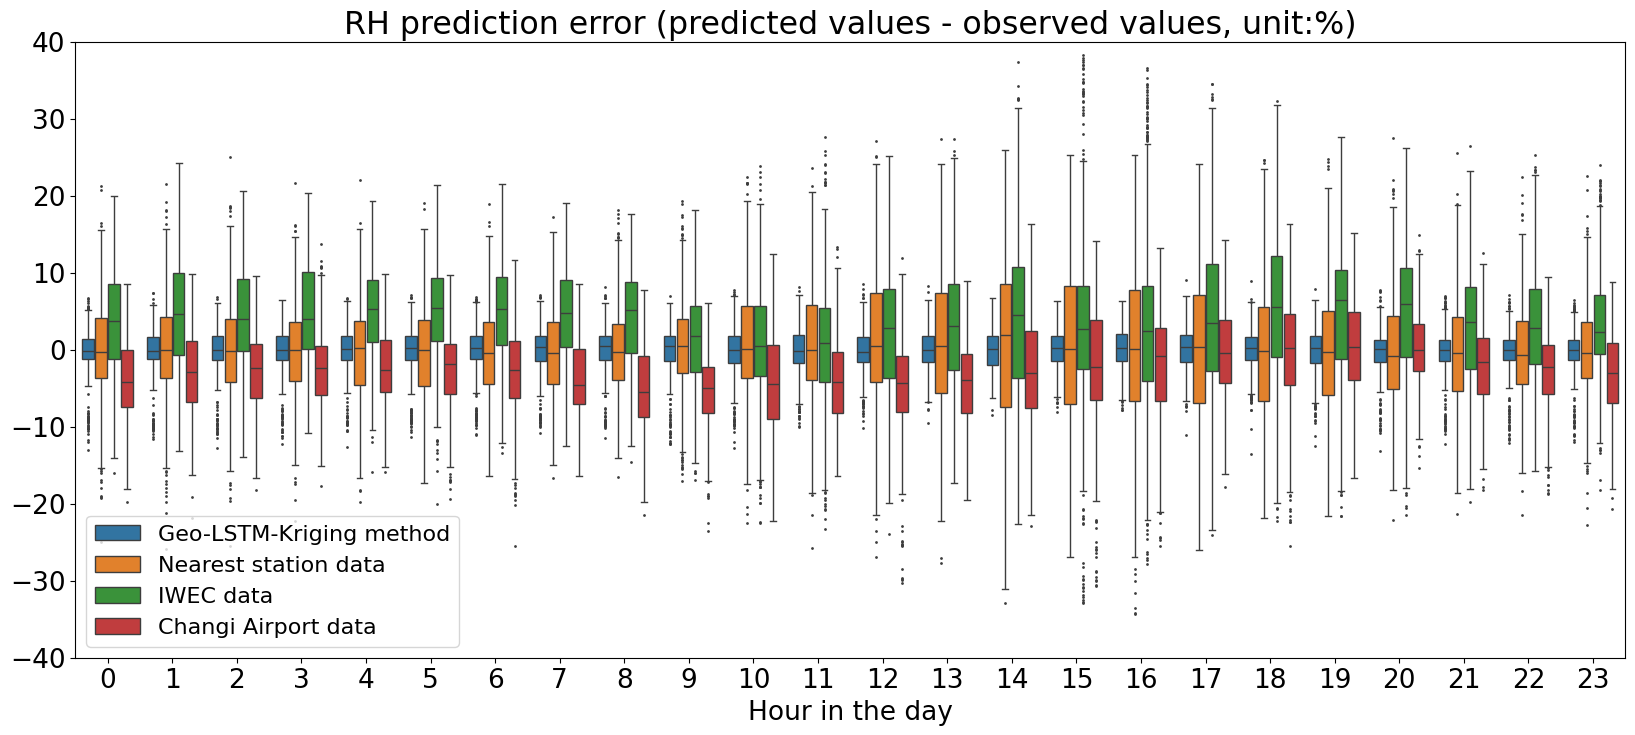
\includegraphics[scale=0.38]{figs/new_figs/RHrk_ne_airport.png}
    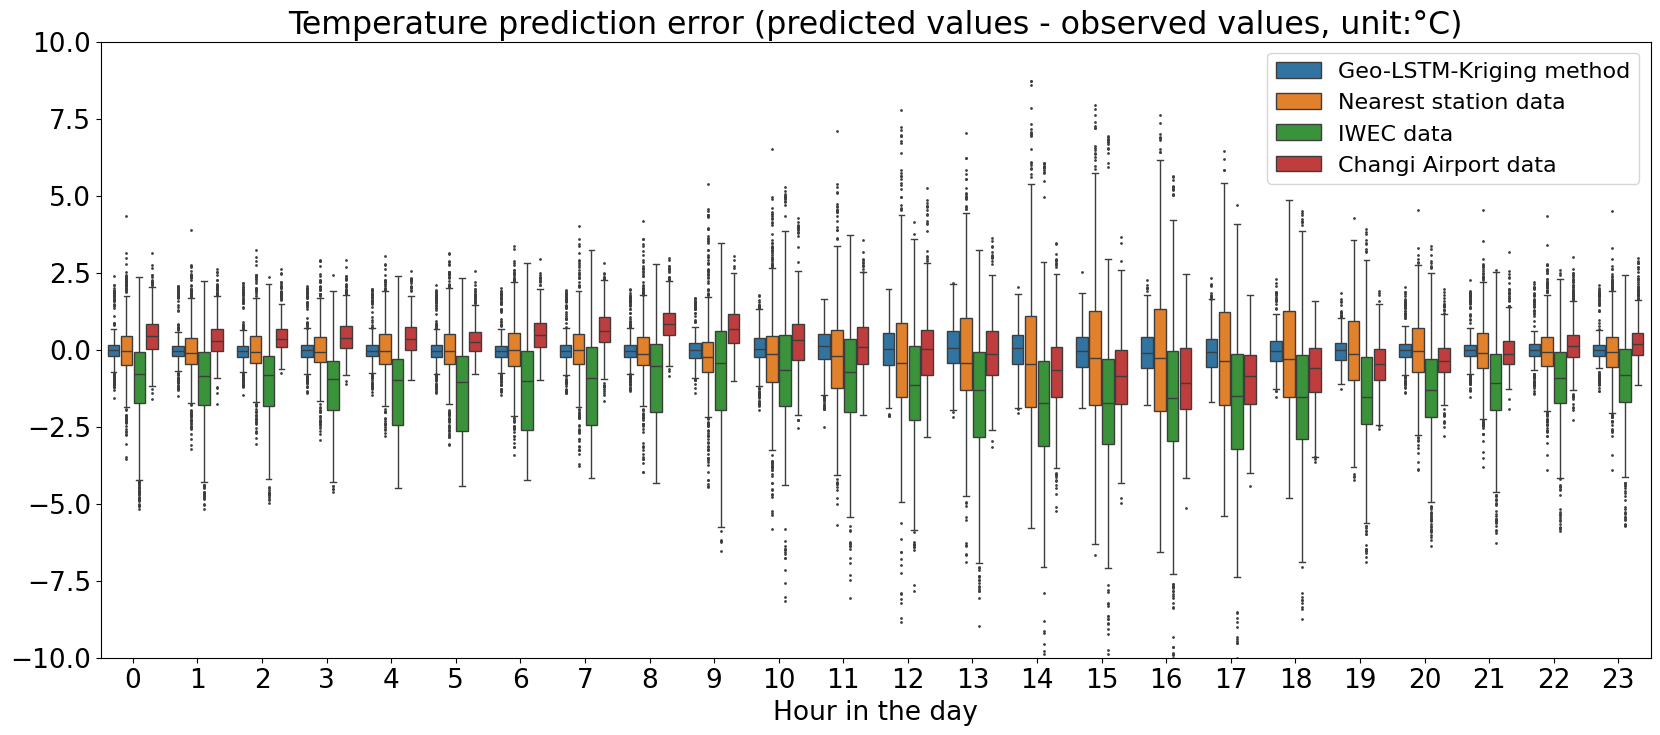
\includegraphics[scale=0.38]{figs/new_figs/TEMrk_ne_airport.png}
	\caption{Temporal comparison between Geo-LSTM-Kriging and practical (level-2) baselines.}
	\label{FIG:baselines2}
\end{figure}

From the above figure, we can observe several intriguing phenomena. The most evident difference lies in the higher humidity and lower temperature observed in the IWEC data compared to the local NUS campus data. We can reasonably speculate that this discrepancy is related to the historical lag in IWEC data. With the intensification of the greenhouse effect, the global warming phenomenon has become increasingly pronounced in recent years. Clearly, conventional meteorological data has become outdated. In studies utilizing typical weather files, researchers should be attentive to this aspect. Existing research indicates that updated typical weather files, compared to outdated ones, can have a significant impact of up to 50-65\% on building energy simulations. \citep{costanzo2020updated}, the issue of weather file outdatedness has become increasingly imperative in studies pertaining to microclimate. On the other hand, a stark contrast in the deviation patterns is discernible when comparing the data from Changi Airport with that of the NUS campus. Changi Airport exhibits a conspicuous disparity, with consistently lower average humidity and higher temperatures. It is noteworthy that temporal consistency between the two datasets was ensured during the plotting process. Therefore, a reasonable inference can be made that such data discrepancies stem from divergent local environmental conditions. In comparison to the open and flat geographical environment of the airport, the NUS campus boasts a higher vegetation coverage. Such geographical conditions have the potential to mitigate issues like UHI effect, thereby reducing surface temperatures. In order to rigorously investigate the influence of various features within the Land Use and Land Cover (LULC) data on the environment and model performance, we will conduct spatial analysis on 14 weather stations in the subsequent section, providing a more quantified theoretical basis.

Additionally, as mentioned in the preceding section, we summarized the overall comparative results of our model and the two-level baseline in Table \ref{tab:RMSE}. The RMSE and variance in the table represent the overall performance across all 14 weather stations for the entire month. Upon observing the table, it is evident that machine learning models exhibit a significant improvement compared to conventional interpolation models (e.g., the RMSE for temperature increased from 1.59 in kriging to 0.70 in LSTM-Kriging, and the R-squared for RH increased from 0.673 in kriging to 0.931 in LSTM-Kriging). We selected a machine learning model with outstanding performance and introduced a geo layer. With the addition of the geo layer, there was an improvement in the RMSE for temperature, decreasing from 0.70 to 0.64, while other indicators showed less pronounced changes. Among the level-2 baselines, the data from Changi Airport performed better but still exhibited a noticeable gap compared to the LSTM-Kriging model. The specific model performance for different weather stations and the correlation with their respective LULC features will be detailed in the next section on spatial analysis.

\begin{table}[width=.9\linewidth,pos=h] 
\caption{RMSE and R-square of the prediction error of different methods.} \label{tab:RMSE}
\centering \small
\begin{displaymath}
\begin{array}{ c || c | c  c  c  c | c  c  c }
\hline
 \rule{0pt}{12pt}
 & & \multicolumn{4}{ c |}{\text{Level 1 baselines}} & \multicolumn{3}{ c }{\text{Level 2 baselines}}\\
  &   \text{Geo-LSTM-K} &   \text{LSTM-K}   & \text{GRU-K}  & \text{Kriging} & \text{IDW}   & \text{Nearest}  & \text{IWEC} & \text{Changi Airport}  \\
\hline \rule{0pt}{10pt}
\text{RMSE (Temp.)/°C} & 0.64 & 0.70 &  0.70 & 1.60 & 1.60 & 1.72 & 2.37 & 1.09  \\
\text{RMSE (RH)/\%} & 3.23 & 3.43 & 3.44 & 7.70 & 7.74 & 8.19 & 9.50 & 6.73  \\
R^2 \text{(Temp.)} & 0.9975 & 0.9950 & 0.9945 & 0.9850 & 0.9848 & 0.9640 & 0.9823 & 0.9930  \\
R^2 \text{(RH)} & 0.9385 & 0.9309 & 0.9306 & 0.6727 & 0.6752 & 0.6362 & 0.6106 & 0.6899  \\
\hline
\end{array}
\end{displaymath}
\end{table}

%We first compared the overall errors, and then we will provide a detailed analysis of the temporal errors. In Figure \ref{FIG:baselines2}, the ground truth of the mean temperature represents the average value of all measured data from weather stations within the campus for the entire month of July 2019. The "Nearest Station" item uses a replacement method where each weather station is substituted with data from its closest weather station, and the average value is calculated accordingly. The "Changi Airport" item represents the average value of the urban weather station measurements at Singapore Changi Airport for the whole month. It is evident that using our high spatial-resolution approach for prediction results in a significant improvement compared to the two traditional methods, especially compared to the urban weather station data.

\iffalse
\begin{table}[width=1.0\linewidth,cols=5,pos=h]
\caption{Comparison with different scales of substitutions of the target station.}\label{Changi airport}
\begin{tabular*}{\tblwidth}{@{} LLLLL@{} }
\toprule
  & Ground Truth & Prediction of our method & Nearest station  &Changi airport\\
\midrule
Mean temperature(\textdegree C) & 28.05 & 28.29& 28.50& 29.51\\
Temperature prediction error & - & 0.86\% & 1.60\% & 5.20\%\\
\bottomrule
\end{tabular*}
\end{table}
\fi

\iffalse
\begin{figure}[!h]
	\centering
	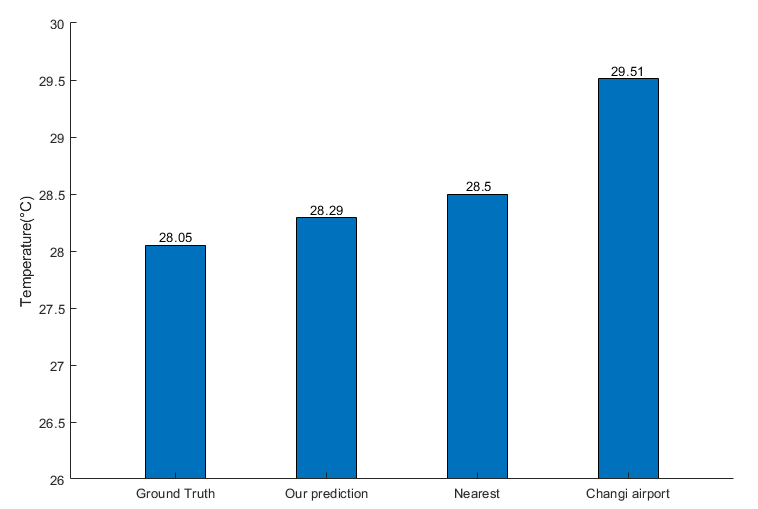
\includegraphics[scale=0.6]{figs/ComparisonWithLevel2.png}
	\caption{Comparison with different microclimate prediction or estimation methods }
	\label{FIG: ComparisonLevel2}
\end{figure}
\fi

%To further compare the differences between our proposed model and the direct use of data from the nearest weather stations in practical application scenarios, we summarized the results of the nearest weather station in Table \ref{comparison with nearest}. This table includes the observed values of relative humidity (RH) and temperature, the predicted values from both models, and the improvement in Mean Absolute Error (MAE). The results show that our model exhibits varying degrees of improvement compared to the nearest model across different weather stations, ranging from 0.96\% to 42.94\%. The degree of improvement is significantly correlated with the actual LULC conditions of each weather station. This indicates that typical urban weather data can only provide a rough reference to microclimate characteristics. In a high-resolution spatial range, geographical environmental features have a significant impact on localized microclimate characteristics.

\iffalse
\begin{table}[width=.9\linewidth,cols=4,pos=h]
\caption{Analysis of prediction error fluctuations (Time period 1-6 represents 0-4 a.m., 4-8 a.m., 8-12 p.m., 12-4 p.m., 4-8 p.m., 8-12 p.m. respectively)}\label{std_analysis}
\begin{tabular*}{\tblwidth}{@{} LLLLLLL@{} }
\toprule
Time period in the day & 1 & 2 & 3 & 4 & 5 & 6\\
\midrule
Geo-LSTM-K Tem prediction error std & 0.598 &0.584 &0.631 &0.801  &0.65 & 0.559\\
LSTM-K Tem prediction error std & 0.648 &0.623 &0.705  &0.855 &0.723 & 0.624\\
Geo-LSTM-K Tem prediction max positive error & 2.403& 2.110& 1.971& 2.520&  2.322&  2.27\\
LSTM-K Tem prediction max positive error & 2.335& 2.078& 2.32& 2.229& 2.226& 2.398\\
Geo-LSTM-K Tem prediction min negative error & -1.578& -1.462& -2.511& -2.189& -1.785& -1.531\\
LSTM-K Tem prediction min negative error & -1.758& -1.594& -2.643& -2.528& -2.335& -1.856\\
\midrule
Geo-LSTM-K RH prediction error std & 3.450& 3.433& 3.459&  2.803& 2.898&  3.266\\
LSTM-K RH prediction error std & 3.767& 3.689& 3.756&2.809& 2.939& 3.485\\
Geo-LSTM-K RH prediction max positive error & 7.409& 7.156& 8.155& 8.481& 9.104& 7.785\\
LSTM-K RH prediction max positive error &  8.331&  8.219& 12.03&  9.756& 10.094&  8.400\\
Geo-LSTM-K RH prediction min negative error & -13.09& -12.61& -12.80& -10.21& -13.53 &
 -13.09\\
LSTM-K RH prediction min negative error & -12.96& -12.00& -14.46&  -9.07& -12.17&
 -12.07\\
	
\bottomrule
\end{tabular*}
\end{table}
\fi

%In addition to the mean values of each weather station, we further compare and analyze the prediction errors with the nearest baseline for three representative weather stations mentioned in the previous section. According to Figure \ref{FIG:TEMRH_3Stations}, we can observe that various machine learning models consistently outperform the nearest baseline, and the differences are significant. Compared to the natural nearest model, our Geo-LSTM-Kriging model reduces the MAE of RH from 8.2 to 5.1 at station 8 and the MAE of temperature from 1.7\textdegree C to 1.1\textdegree C at the same station. The LULC data of station 8 is much different from its neighbors, so the natural nearest model performs the worst here among all the stations. At stations 7 and 12, the improvement of machine learning methods is less significant, with the MAE of RH from 1.9 to 1.6 and from 2.1 to 0.8, respectively, and the MAE of temperature from 0.7\textdegree C to 0.5\textdegree C and from 0.4\textdegree C to 0.2\textdegree C respectively. 

\iffalse
\begin{figure}[!h]
	\centering
	\includegraphics[scale=0.55]{figs/RHTEM_3stations.png}
	\caption{Mean relative absolute error and R squared of temperature and RH at stations 7, 8, and 12.}
	\label{FIG:TEMRH_3Stations}
\end{figure}
\fi




%Figure \ref{FIG: daily} and Figure \ref{FIG: hourly} illustrate the variations in daily and hourly average temperatures between Geo-Kriging-LSTM and other Level 2 baselines. It is evident that Changi Airport's data differs the most from the actual measurements. Airport data is unable to replicate the non-linearities in temperature data, although some general trends are captured, the more extreme changes, especially peaks and troughs, are excluded. The proposed model shows a much better alignment with the actual measured values and can accurately capture daily variations. It is the best match among all models, excelling at capturing daily changes and irregularities.

\iffalse
\begin{figure}[!h]
	\centering
	\includegraphics[scale=0.6]{figs/timeseriesdaily.png}
	\caption{Daily average result of different prediction methods.}
	\label{FIG: daily}
\end{figure}\begin{figure}[!h]
	\centering
	\includegraphics[scale=0.6]{figs/timeseries.png}
	\caption{Hourly performance of different prediction methods.}
	\label{FIG: hourly}
\end{figure}
\fi


\iffalse
\begin{table}[width=.9\linewidth,cols=4,pos=h]
\caption{Geo-LSTM-Kriging weather prediction model in different scales.}\label{use case of weather sensor placement description}
\begin{tabular*}{\tblwidth}{@{} LL@{} }
\toprule
Case name & Case description\\
\midrule
Neighbors5 & default scale, using 5 nearest other stations to train\\
\midrule
Neighbors3 & using 3 nearest other stations to train\\
\midrule
LULC-Neighbors3 & \begin{tabular}[c]{@{}l}using 3 of the 5 nearest other stations \\whose LULC are the closest to the target station\end{tabular}\\
\bottomrule
\end{tabular*}
\end{table}
\fi



\subsection{Model spatial performance analysis}

After analyzing the temporal aspects of the prediction results, we proceeded with a comprehensive spatial analysis based on the different geographical conditions. We calculated the prediction errors for all 14 stations and found that their trends over time vary among different weather stations. Therefore, we categorized these weather stations according to temporal prediction error at their spatial locations' performance including both temperature and RH prediction errors. Such classification results are further analyzed combined with their LULC features, to explore the potential pattern of the environmental effects. 


In the actual classification process, we treated the prediction errors of temperature and humidity for each hour of every day within a month at each weather station as a time series data point. We aggregated these data points and performed clustering. Specifically, for instance, if, among the 30 data points for Weather Station 1, 20 belong to cluster 0 and 10 belong to category 1, then we conclude that Weather Station 1 has 1/3 of its attributes belonging to category 1 and 2/3 belonging to category 0 (this is a simplified example for illustration purposes and is not related to actual results). Figure \ref{FIG:clusterError} illustrates the clustering results obtained using the DTW algorithm, as mentioned in Section \ref{DTW}. Different colors represent the temporal performance of prediction errors for different clusters of weather stations. The left panel represents humidity prediction errors, while the right panel represents temperature prediction errors. It is noteworthy that only Weather Station 8 is in cluster 0, and it exhibits higher errors in all the models including baselines compared to other weather stations. In Figure 2, a comparison is made between the actual measurements of Weather Station 8 and those of other weather stations. It is evident that the actual data for Weather Station 8 differs significantly from the data of other weather stations across the campus. Its temperature is consistently lower throughout the 24 hours, and the humidity is higher. Hence, the higher prediction errors when using other weather stations for interpolation can be explained. 

Figure \ref{FIG:Result of DTW clustering} shows the overall classification results, where PCA was employed to reduce data dimensionality, transforming the 24-dimensional time series data into two dimensions (x and y) for better observation of the clustering results. Here, we observe that cluster 0 (depicted in blue), representing Weather Station 8, is distant from the other weather stations, while the other three clusters exhibit certain degrees of cohesion, which indicates the classification results are deemed reasonable.

Upon further examination of Figure \ref{FIG:clusterError}, it becomes evident that, apart from the isolated Weather Station 8, the other three categories of weather stations also exhibit distinct trends in prediction errors. In cluster 1 (depicted in orange), the prediction error for RH is lower during the midday period (10:00-14:00), while the prediction error for temperature is higher during this interval. Cluster 2 (depicted in green) demonstrates relatively stable prediction errors throughout the entire period. Conversely, cluster 3 (depicted in red) exhibits trends opposite to those in cluster 1. To delve deeper into the correlation between prediction errors across different clusters and the corresponding LULC features of various weather stations, we further employed PCA to reduce data dimensionality and generated Figure \ref{fig:DTWclusteringLULCdata}. In this figure, the x-axis represents the values of the principal components obtained through PCA for the reduced dimensionality of time series prediction errors at all the weather stations, while the y-axis in each subfigure represents the values of different LULC features. In general, the relationship between prediction errors and LULC features is intricate, making simple correlation assessments unfeasible. However, certain features manifest more pronounced influences in specific instances. In Table \ref{tab:LULC_label}, we summarize several features that exhibit differences in performance among weather stations in different clusters. We can observe differences in these features among different categories (excluding the standalone cluster 0). The varying distances to buildings and walkways imply differences in shading conditions at different times of the day. For instance, Cluster 1 has an average distance to buildings of approximately 9.7 meters, while Cluster 3 has an average distance of about 23.09 meters. This suggests that buildings may provide more shading for Category 1, causing weather stations in Category 1 to exhibit larger fluctuations during the noon period. The observed discrepancies between the model predictions and the actual conditions, with lower humidity and higher temperature in our predictions, might be attributed to the incomplete learning of the impact of building shadows. However, due to the limited number of weather stations, a more systematic quantitative analysis is not feasible, and we can only provide a qualitative and reasonable inference. We can infer that these features likely have varying degrees of influence on predictions for different weather stations and different time periods.

Due to the limited number of weather stations in this study, there are notable constraints on the correlation analysis between clustering results and LULC features. Nevertheless, within the restricted dataset of 14 weather stations, we have identified certain patterns, indicating that different LULC features exert varying degrees of influence on model performance. These features provide distinct environmental conditions for the target locations, leading to diverse manifestations of urban heat island effects, urban heat exchange, urban surface characteristics, and other related factors. Consequently, these impacts are reflected in the model prediction performances, resulting in diverse levels of errors and stability. The associated effects merit further investigation in future studies involving a more extensive array of weather stations.


\begin{figure}[!h]
	\centering
	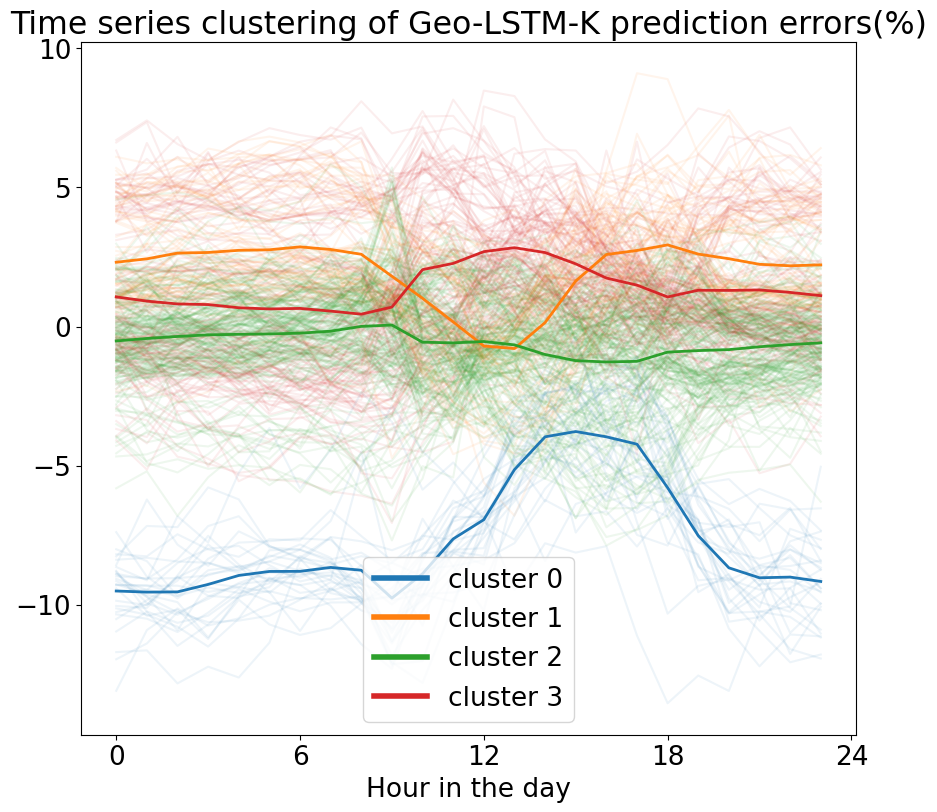
\includegraphics[scale=0.22]{figs/new_figs/RHerrorclustering.png}
	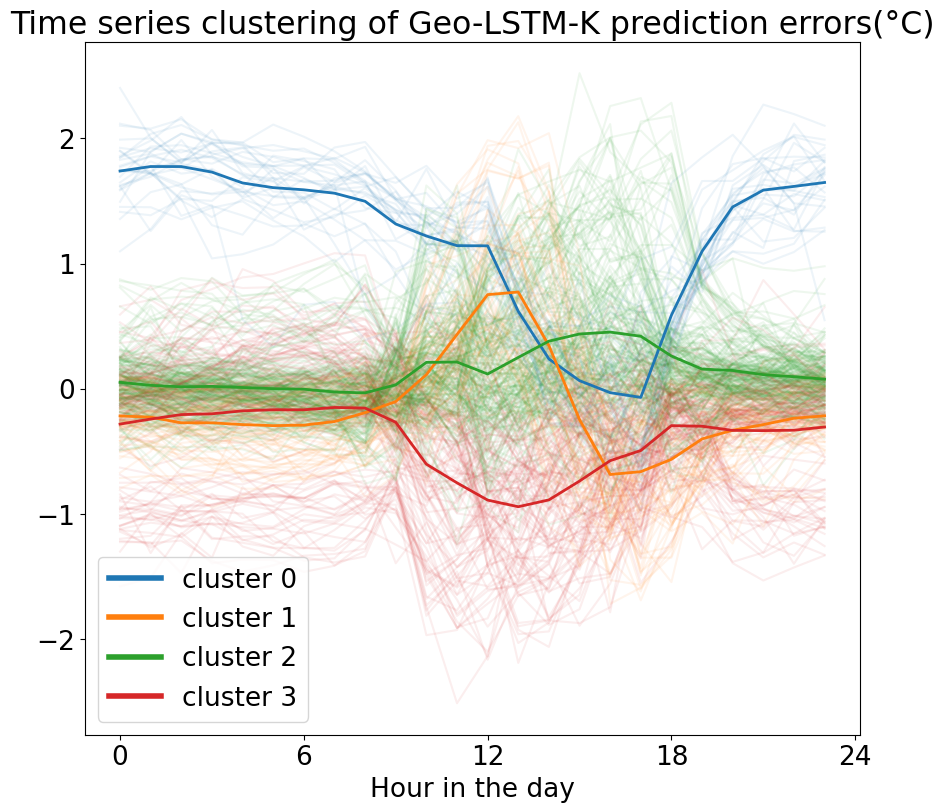
\includegraphics[scale=0.22]{figs/new_figs/TEMerrorclustering.png}
	\caption{Clustering of weather stations based on the prediction errors.}
	\label{FIG:clusterError}
\end{figure}

\begin{figure}[!h]
	\centering
        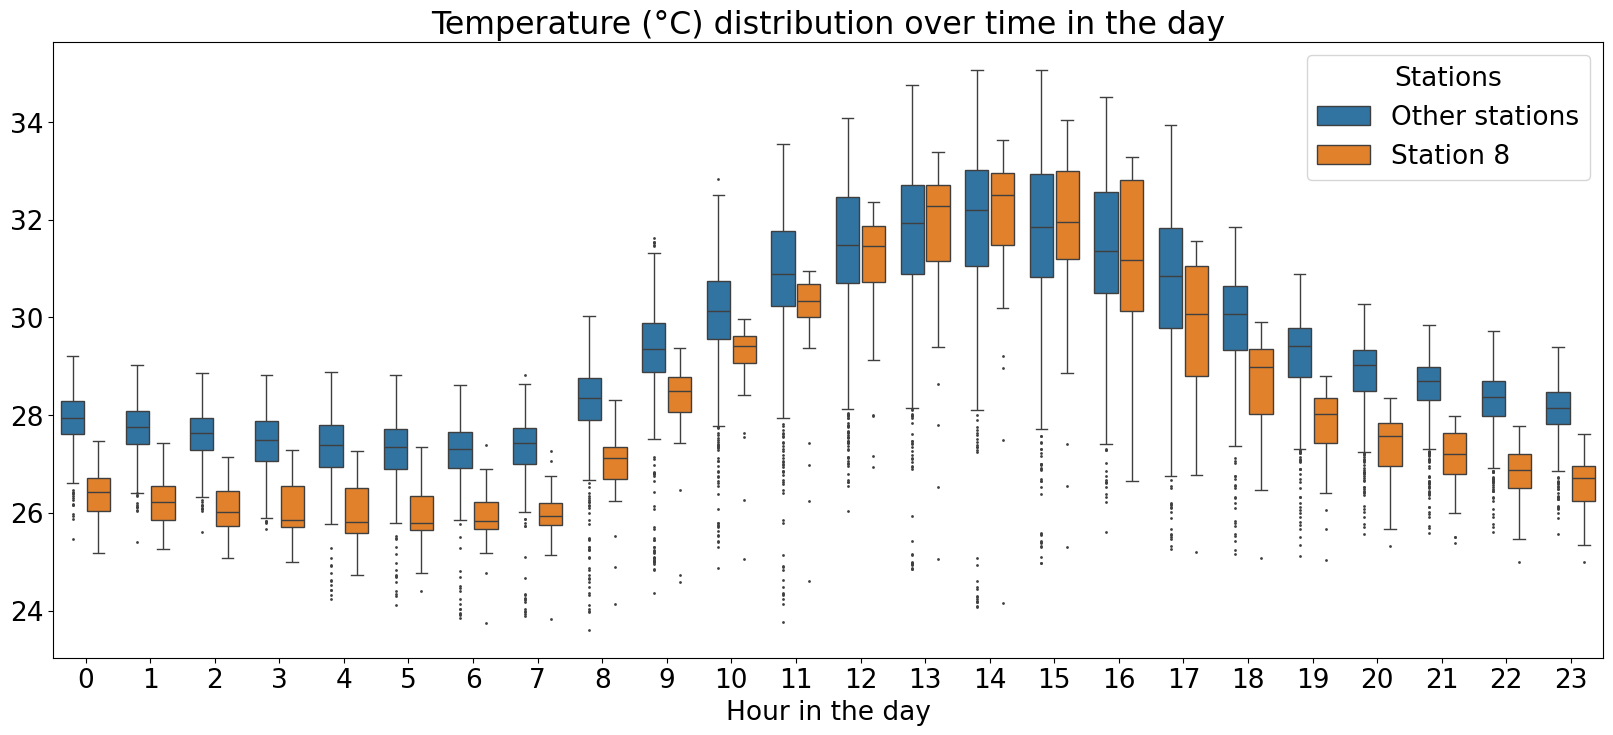
\includegraphics[scale=0.25]{figs/new_figs/station8tem.png}
        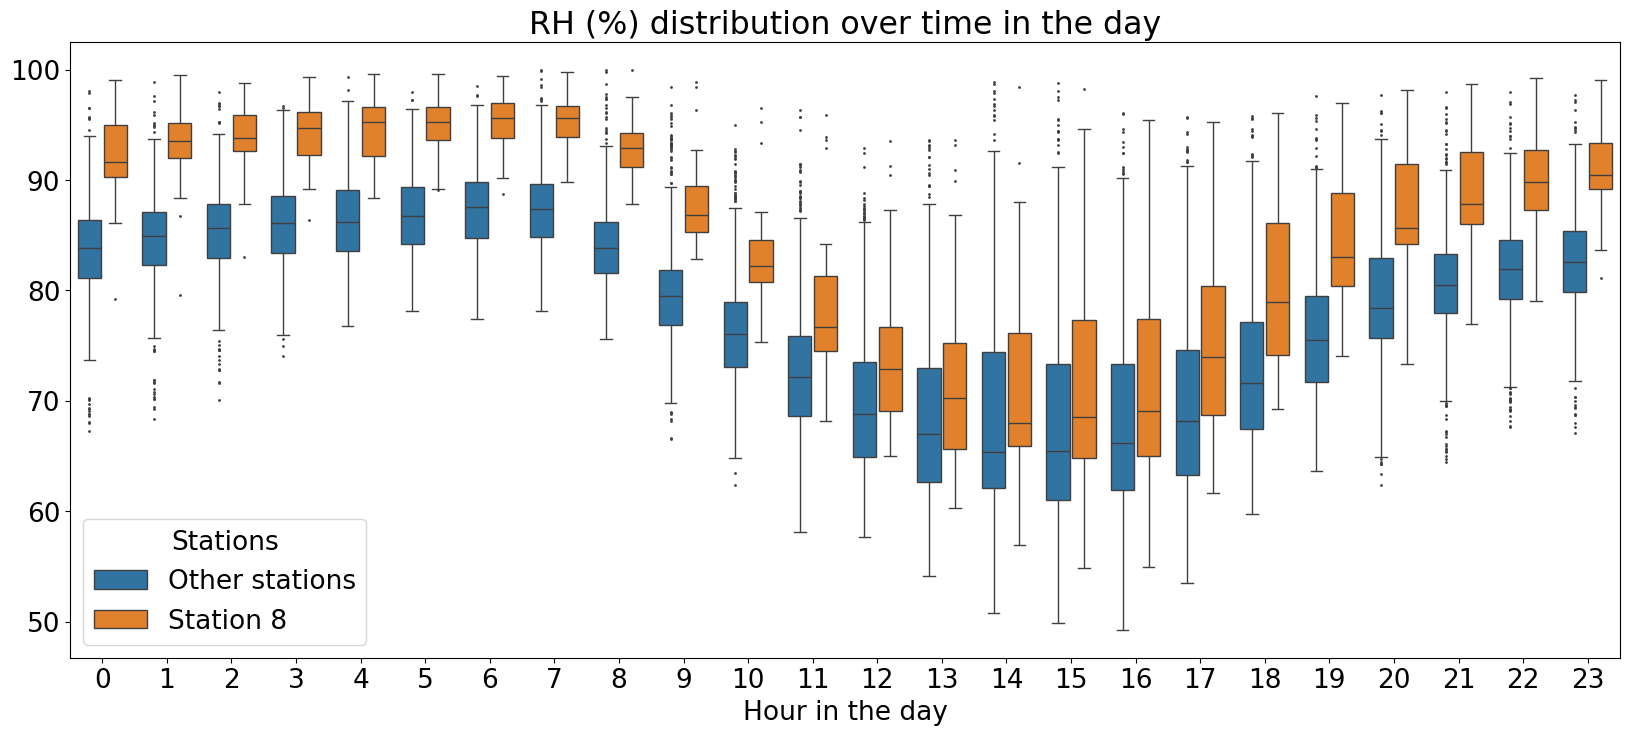
\includegraphics[scale=0.25]{figs/new_figs/station8RH.png}
	\caption{Comparison of the temperature data of station 8 with all the other stations}
	\label{FIG:station8tem}
\end{figure}


\begin{figure}
	\centering
	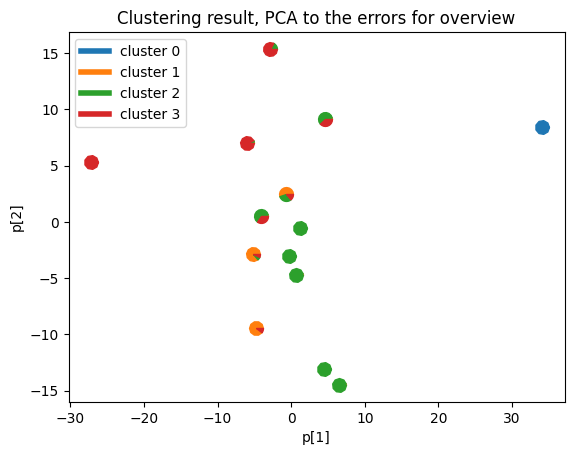
\includegraphics[scale=0.6]{figs/new_figs/clusteringresult.png}
	\caption{Station clustering result based on DTW analysis over the error series at each station location.}
	\label{FIG:Result of DTW clustering}
\end{figure}


\begin{figure}
    \centering
    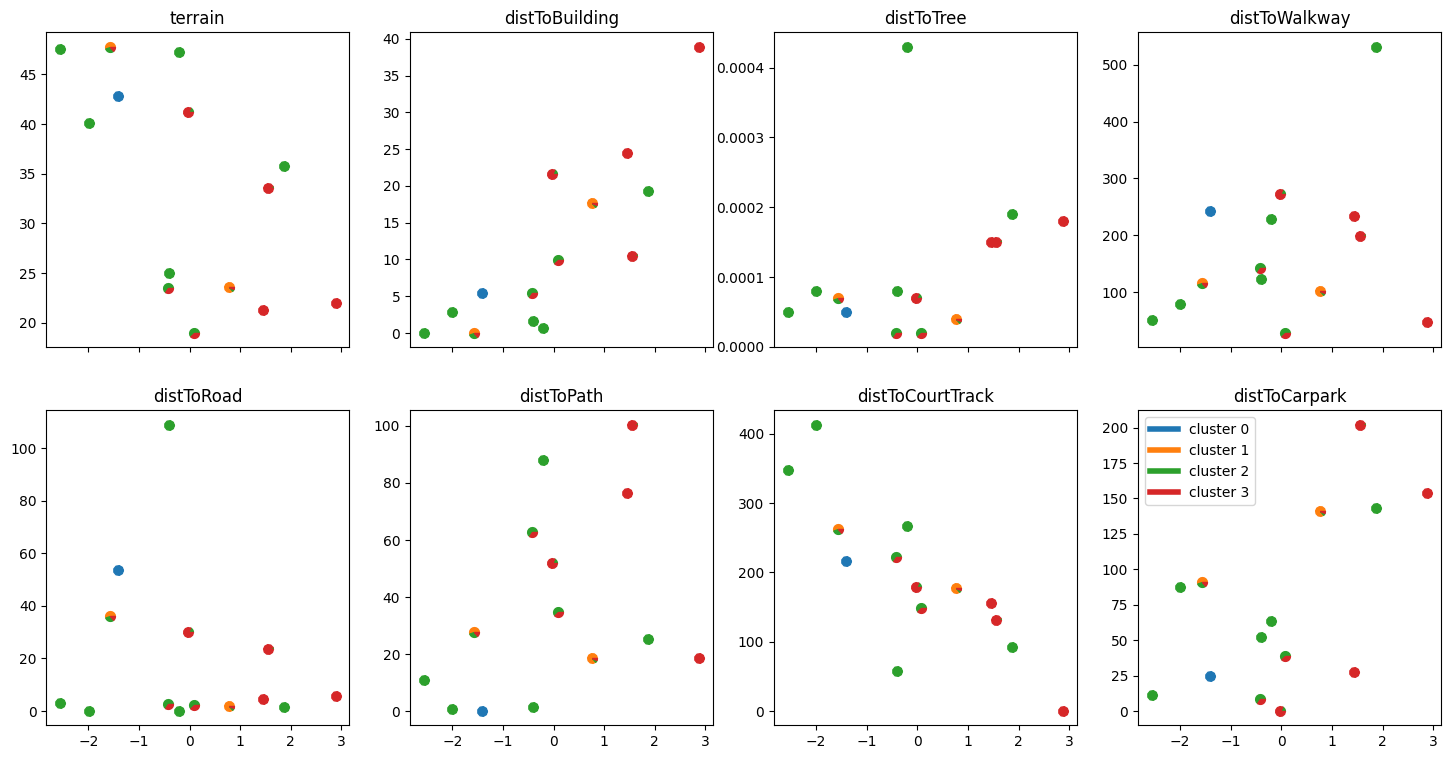
\includegraphics[scale=0.4]{figs/new_figs/clusterLULCplot.png}
    \caption{The distribution of LULC features and PCA values of stations in each cluster.}
    \label{fig:DTWclusteringLULCdata}
\end{figure}

\begin{table}[width=.45\linewidth,pos=h]
    \caption{LULC feature data.}
    \label{tab:LULC_label}
    \centering
    \begin{tabular}{c | c c c c}
    \toprule
         Cluster id & 0 & 1 & 2 & 3 \\
    \midrule
         Terrain std& 10.4 & 10.6 & 8.9 & 7.5 \\
         Terrain mean& 35.1 & 30.9 & 38.2 & 25.4 \\
         DistToBuilding std& 6.5 & 6.7 & 7.7 & 11.9 \\
         DistToBuilding mean& 9.08 & 9.70 & 5.94 & 23.09 \\
         DistToWalkway std& 81.74 & 69.00 & 161.40 & 87.85 \\
         DistToWalkway mean& 173.96 & 130.48 & 194.34 & 145.03 \\
         \bottomrule
    \end{tabular}
\end{table}

%In order to provide a more comprehensive assessment of our model, we summarize the improvement provided by different layers in Table \ref{comparison of the improvement given by different layers}. It is evident that the Kriging layer plays the most critical role in the network structure, while the LSTM layer and Geo-layer follow behind with similar effects. 

\iffalse
\begin{table}[width=.9\linewidth,cols=4,pos=h]
\caption{Comparison of the improvement given by different layers.}\label{comparison of the improvement given by different layers}
\begin{tabular*}{\tblwidth}{@{} LLLLLLLL@{} }
\toprule
Station number &  1 & 2 & 3 & 4 & 5& 6 & 7\\
\midrule
True RH mean value & 72.83 & 70.79 & 70.86 & 71.37 & 73.15& 74.62 & 71.59\\
LSTM-layer MRE difference & 
4.87\%&5.14\%&6.21\%&1.18\%&3.86\%& 5.19\%&5.25\%\\
Kriging-layer MRE difference & 
6.72\%&6.20\%&7.92\%&5.70\%&3.25\%& 5.64\%&8.38\%\\
Geo-layer MRE difference&2.07\%&2.06\%&3.69\%&2.46\%&2.24\%&2.05\%&3.34\%\\
\midrule
True temperature mean value(\textdegree C) & 29.20 & 29.52 & 29.30 & 29.50 &28.91& 29.44 & 29.24\\
LSTM-layer MAE difference(\textdegree C) & 0.44&0.18&0.31&0.28&0.25& 0.40&0.21\\
Kriging-layer MAE difference(\textdegree C)&0.17&0.09&0.03&0.06&0.03 &0.17&0.11\\
Geo-layer MAE difference(\textdegree C)&0.04&0.04&0.09&0.01&0.10&0.04&0.05\\
\bottomrule
\end{tabular*}
\begin{tabular*}{\tblwidth}{@{} LLLLLLLL@{} }
\toprule
Station number & 8 & 9 & 10 &  11 & 12 & 13 & 14\\
\midrule
True RH mean value  & 92.63 & 73.39 & 73.26& 83.34 & 76.96 & 82.35 & 74.67\\
LSTM-layer MRE difference &5.35\%&4.24\%&2.36\%&6.31\%&8.92\%&5.13\%&5.76\%\\
Kriging-layer MRE difference &6.41\%&3.02\%&3.57\%& 6.95\%&3.96\%&5.84\%&5.02\%\\
Geo-layer MRE difference&4.73\%&2.04\%&0.56\%&1.05\%&2.16\%&3.23\%&1.58\%\\
\midrule
True temperature mean value(\textdegree C)  & 28.34 & 29.65 &29.12& 29.44 & 29.24 & 28.34 & 29.65\\
LSTM-layer MAE difference (\textdegree C)&0.34&0.25&0.19& 0.45&0.28&0.42&0.48\\
Kriging-layer MAE difference(\textdegree C)&0.02&0.03&0.10&0.17&0.16&0.23&0.19 \\
Geo-layer MAE difference(\textdegree C)&0.08&0.04&0.05&0.08&0.11&0.15&0.23\\
\bottomrule
\end{tabular*}
\end{table}
\fi




%We performed a more in-depth analysis of the performance and enhancement effects of the Geo-layer by integrating geographical information from various weather stations into Table \ref{Comparison of the maximal improvement given by Geo-layer}. Our results demonstrate that the Geo-layer significantly improves the accuracy of temperature and humidity predictions, with the greatest enhancements observed during the afternoon. Additionally, from Figure \ref{FIG:TEMRH_3Stations} of Section \ref{4.2.2}, we observed that the predictive performance of Station 8 is significantly worse compared to the other stations. Here, we can identify a possible reason for this observation. Station 8 is located relatively far away from the other stations (as shown in Figure \ref{FIG:map}) and it also has a high turning percentage. Moreover, the surrounding stations (Station 9 and 10) exhibit significant environmental differences compared to Station 8. These factors make it challenging for the interpolation model to accurately estimate the data for Station 8.


\iffalse
\begin{table}[width=.9\linewidth,cols=4,pos=h]
\caption{Comparison of the maximal improvement given by Geo-layer. MAE improvement is computed as the MAE difference between the two methods divided by the MAE of the LSTM-Kriging method.}\label{Comparison of the maximal improvement given by Geo-layer}
\begin{tabular*}{\tblwidth}{@{} LLLLLLLL@{} }
\toprule
Station number &  1 & 2 & 3 & 4 & 5 &  6 & 7\\
\midrule
Turfing percentage & 64.3\% &10.7\% &0\% & 21.4\% &0\%& 0\% &0\% \\
Building percentage & 35.7\% &78.6\% &100\% & 78.6\% & 0\%& 50.7\% &0\%\\
Pavement percentage& 0\% & 10.7\% &0\% &0\% &100\% & 49.3\% &100\% \\
\midrule
RH maximal improvement time& 18:00 &  15:00& 13:00 & 18:00 & 6:00 & 14:00 &  13:00\\
True RH value & 95 & 92 & 88 & 80 & 86& 94 & 62 \\
LSTM-Kriging prediction value & 90.5 & 86.6 & 84.2 & 84.5&82.4& 90.2 &64.0\\
Geo-LSTM-Kriging prediction value & 92.5 & 88.9 & 86.5 & 83.0&84.4& 92.8 & 63.3\\
Geo-layer MAE improvement & 44.44\%  & 42.60\% & 60.53\% & 33.33\% & 55.56\%& 68.42\%  & 35.00\%\\
\midrule
temperature maximal improvement time & 13:00 & 15:00 & 14:00 & 15:00 & 14:00& 14:00 & 14:00\\
True temperature value($^\text{o}$C) & 28.5 & 27.2 & 24.8 & 25.4 &28.1& 29.3 & 27.2 \\
LSTM-Kriging prediction value($^\text{o}$C) & 26 & 25.3 & 22.3&21.8 &28.4& 28.1 & 25.8 \\
Geo-LSTM-Kriging prediction value($^\text{o}$C) & 26.5 & 25.7 &22.8& 22.2& 28.3 & 28.6 & 26.0 \\
Geo-layer MAE improvement & 20.00\%  & 21.05\%  &20.00\% & 11.11\% & 33.33\% & 41.67\%  & 14.29\%\\
\bottomrule
\end{tabular*}
\begin{tabular*}{\tblwidth}{@{} LLLLLLLL@{} }
\toprule
Station number & 8 & 9 & 10&  11 & 12 & 13 & 14\\
\midrule
Turfing percentage &96.7\% & 0\% &0\% & 33.4\% &0\% &28.4\% & 26.1\% \\
Building percentage  &0\% & 32.5\% & 0\% & 32.5\% &0\% &71.6\% & 73.9\%\\
Pavement percentage &3.3\% &67.5\% &100\%& 34.1\% &100\% &0\% &0\%\\
\midrule
RH maximal improvement time & 11:00 & 12:00 & 14:00 & 14:00 &  14:00& 12:00 & 12:00\\
True RH value & 95 & 88 & 72& 98 & 78 &  85& 82 \\
LSTM-Kriging prediction value  & 78.6 & 85.4&68.9& 94.2 &75.0 & 83.6 & 85.6\\
Geo-LSTM-Kriging prediction value  & 82.4 & 86.2&69.5& 97.3 & 76.3 & 84.4 & 83.2\\
Geo-layer MAE improvement  & 23.18\% & 30.77\% & 19.36\%& 81.58\%  & 43.33\% & 57.14\% & 66.67\%\\
\midrule
temperature maximal improvement time  & 15:00 & 12:00 & 14:00& 15:00 & 14:00 & 11:00 & 12:00\\
True temperature value($^\text{o}$C) & 25.6 & 25.7 &28.3 & 27.5 & 29.3 & 29.6 & 28.4\\
LSTM-Kriging prediction value($^\text{o}$C) & 23.2&23.6 &25.7& 28.0 & 27.9 & 27.5&27.3\\
Geo-LSTM-Kriging prediction value($^\text{o}$C)&24.2& 24.2& 27.0& 27.8 & 28.3 &28.1& 27.8\\
Geo-layer MAE improvement &41.67\% & 28.57\% & 50.00\%& 40.00\%  & 28.57\%  &28.57\% & 45.45\%\\
\bottomrule
\end{tabular*}
\end{table}
\fi

%Notably, despite the varying environmental conditions surrounding each weather station, with some having a higher proportion of built-up areas (e.g., Station 4) and others having a greater proportion of greenery (e.g., Station 2), the Geo-layer effectively learned and accounted for the impact of these obstacles, leading to even more pronounced enhancements in predictive accuracy when the proportion of obstacles was relatively high.



%After conducting the temporal analysis in the preceding section, we present an overview of the model's performance in Table \ref{Overall model analysis}. This table encapsulates the strengths and weaknesses observed in all the experiments conducted thus far. Notably, all the models exhibit suboptimal performance during the afternoon, when sunlight is strong and rapidly changing. However, during this period, the Geo-LSTM-Kriging model performs remarkably well, indicating that the Geo-layer is effective in accounting for the effects of nearby obstacles. 

%Additionally, we present the interpolation performance of the model with respect to the spatial distribution of the target stations in Fig. \ref{FIG:map2}. Each circle on the map denotes the location of a station, while the surrounding rectangle delineates the extent of the geographic information system (GIS) data. The figure demonstrates that the model's performance is superior in areas with a higher density of stations and inferior in regions with inadequate surrounding GIS data. These findings are in alignment with a prior expectations and conform to the prevailing understanding of the phenomenon under investigation.


%In order to validate the application scenarios of our model, in this section we will mainly discuss two use cases and compare the practical application of the model proposed in this paper.

%\subsubsection{Use case of Weather Sensor Placement}
%The second use case is that the geographical environment where the target weather station is located can lead to different prediction results. We hope that through this study, we can provide a certain theoretical basis for the selection of future weather station placement. Therefore, we designed several experiments to figure out where the new station should be placed to gain the maximal information. Figure \ref{FIG:different_station_placement} shows that adding stations which has similar geographic data to the target position is the optimal choice. The MAE of each model at each individual station is shown in Table \ref{use case of weather sensor placement description2}.  

\section{Discussion}\label{Discussion}

In this section, we will provide a typical application scenario for the model and some general model performance discussions. 

A commonly used application scenario is to provide high-precision, high-resolution visualized prediction results for the impact of changes in building and environmental conditions on microclimates within a small area. For instance, Figure \ref{FIG:predictionResultCampus} displays the model's predictions for humidity and temperature at three different time points, from top to bottom: the predictions for 04:00 on July 5th, 20:00 on July 9th, and 12:00 on July 22nd. Our model initially learns geographical information through the Geo-Kriging layer. Subsequently, it downscales the historical data from the original weather stations to a finer grid. After that, the LSTM layer is employed to predict and generate this map based on the downscaled data. In this figure, we did not depict any actual buildings or road objects, but the high-density predictions at different time intervals partially reflect the outlines of roads and buildings, especially during the midday period where the temperature predictions essentially outline the distribution of roads within the area. In the ever-changing built environment, such as when urban planners are considering increasing vegetation coverage in a specific area or when certain buildings require renovation, expansion, or demolition, this model can proactively offer detailed temporal results of microclimate data, providing valuable insights for related decision-making.

\begin{figure}[!h]
	\centering
	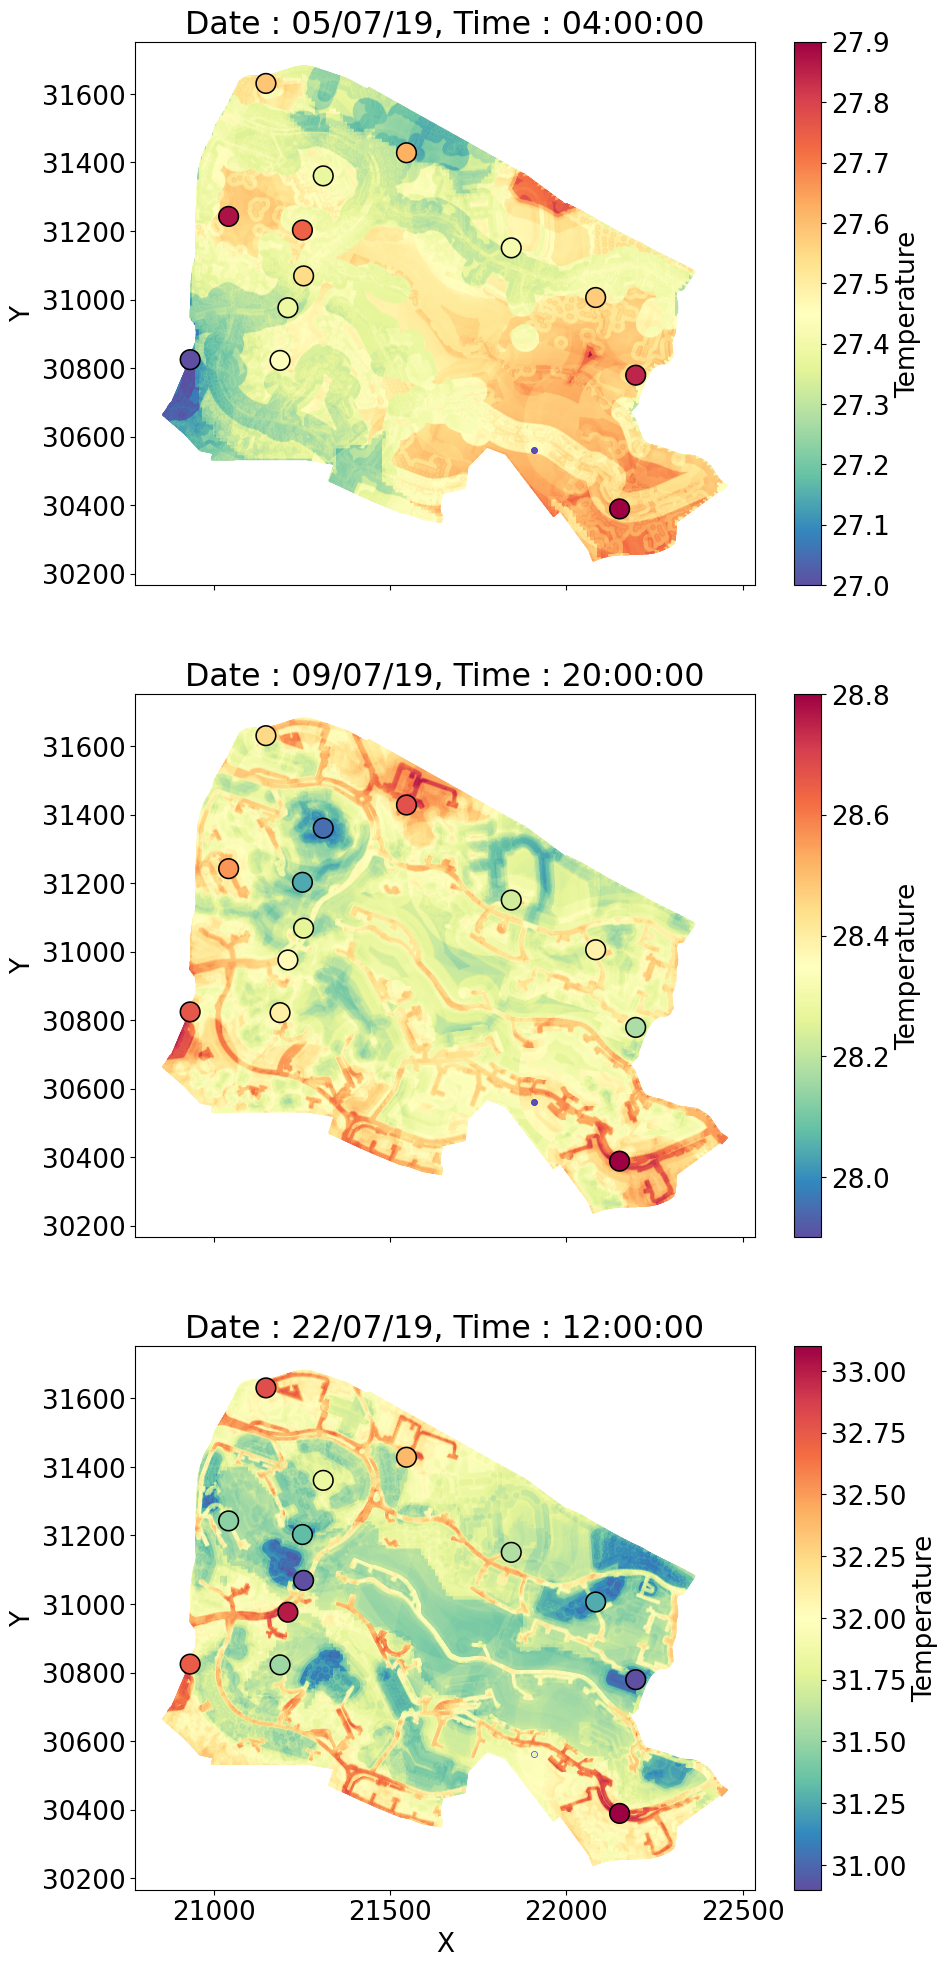
\includegraphics[scale=0.3]{figs/new_figs/tem_campusplot.png}
    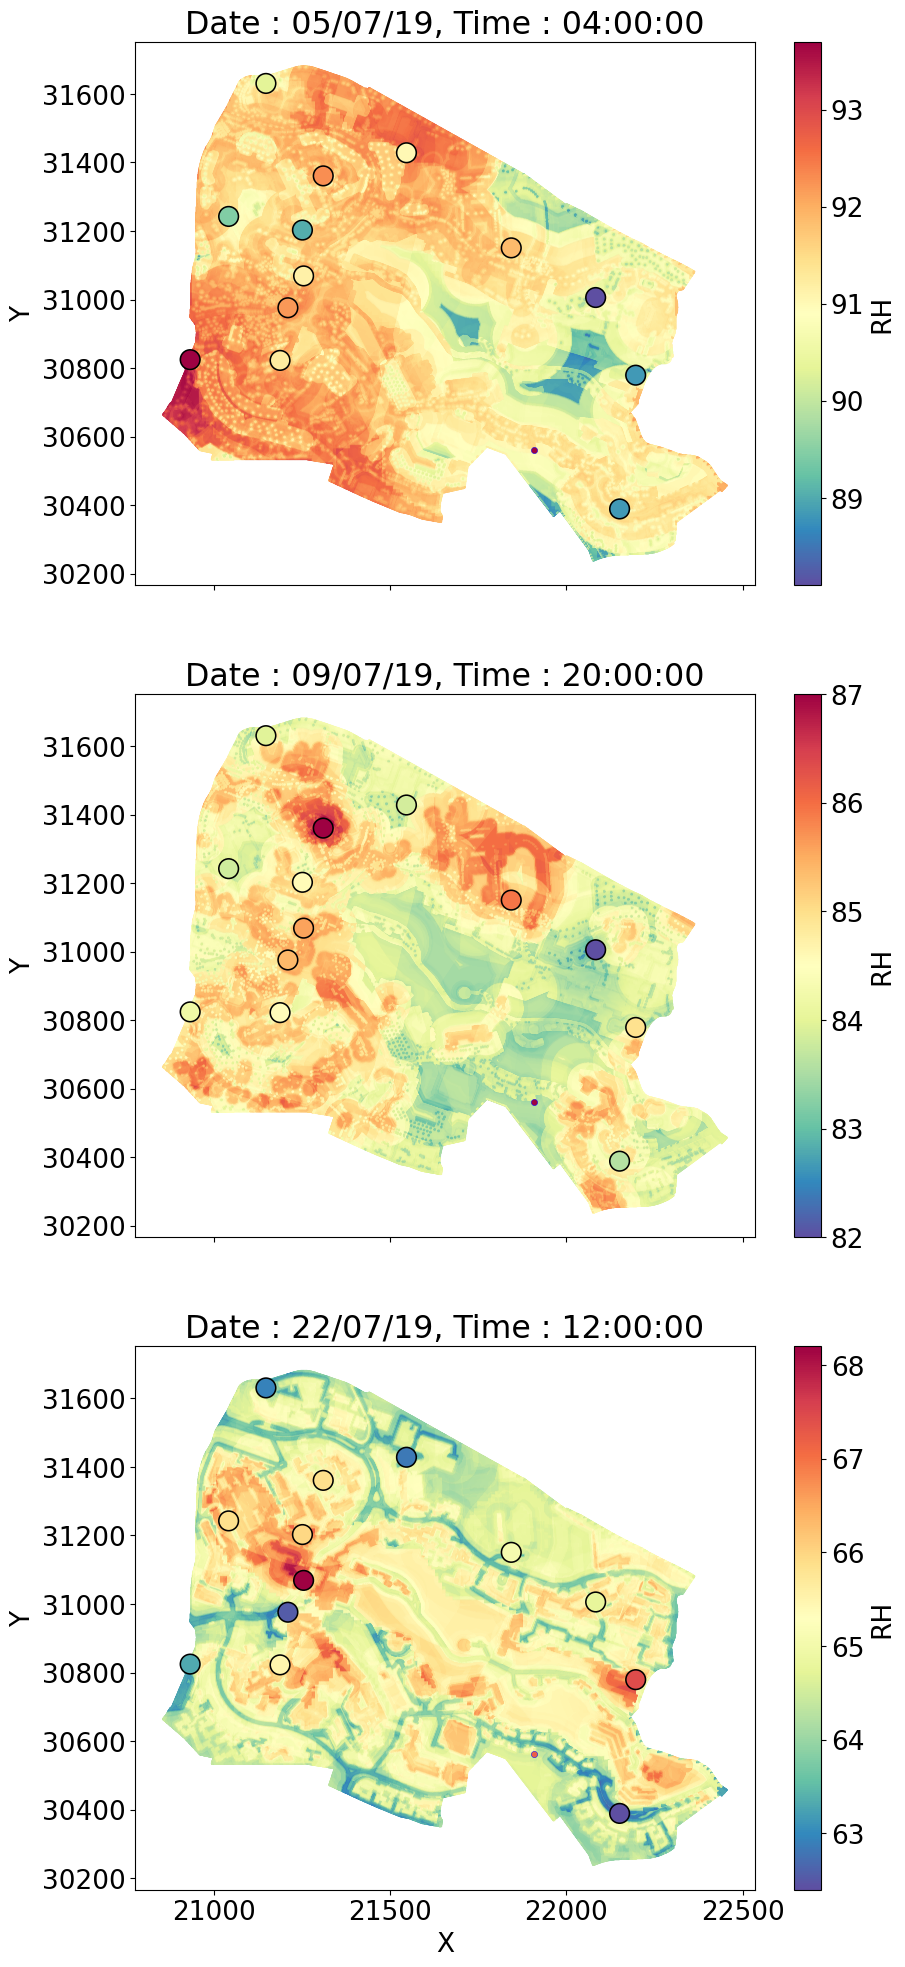
\includegraphics[scale=0.3]{figs/new_figs/RH_campusplot.png}
	\caption{Prediction result samples of Geo-LSTM-Kriging model.}
	\label{FIG:predictionResultCampus}
\end{figure}




\iffalse
\begin{figure}[!h]
	\centering
	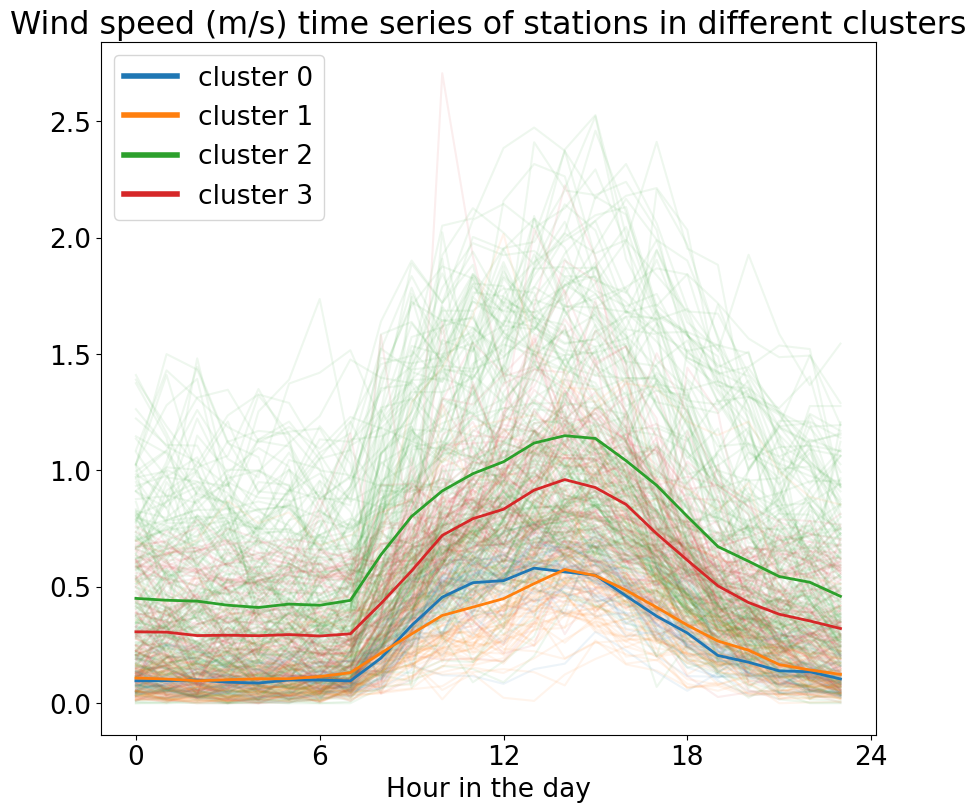
\includegraphics[scale=0.2]{figs/new_figs/windspeed.png}
	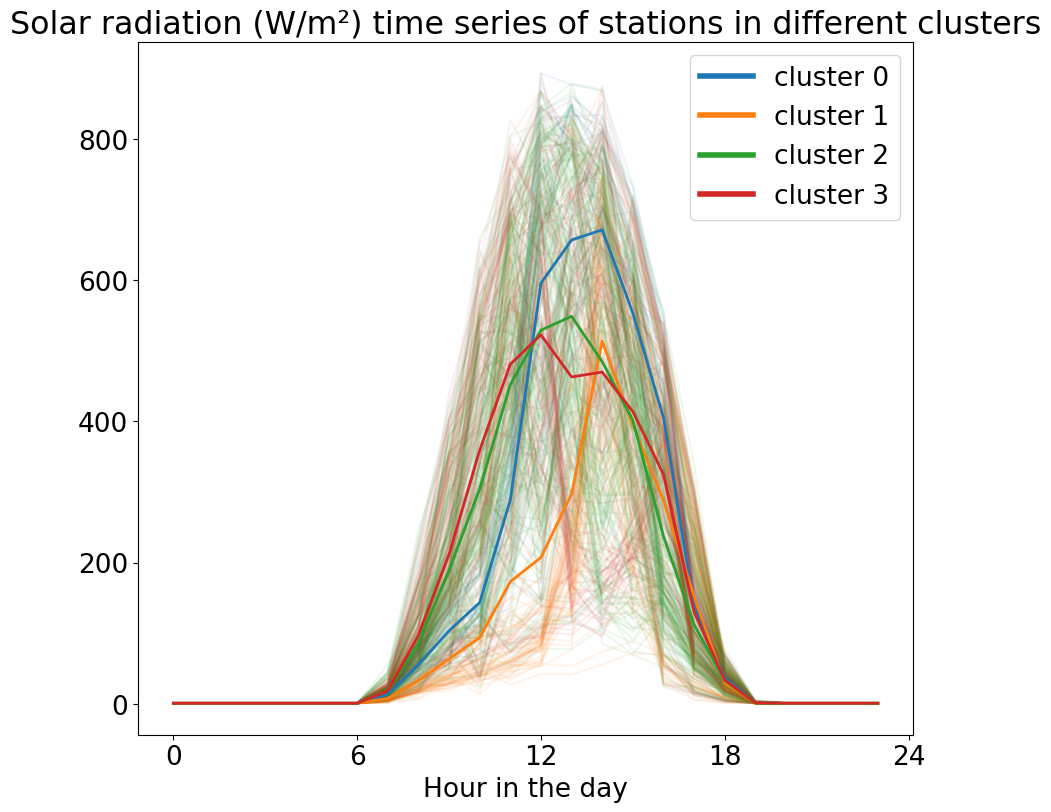
\includegraphics[scale=0.2]{figs/new_figs/solarradiation.png}
	\caption{Clustering of weather stations based on the prediction errors.}
	\label{FIG:windspeedbox}
\end{figure}
\begin{figure}[!h]
	\centering
	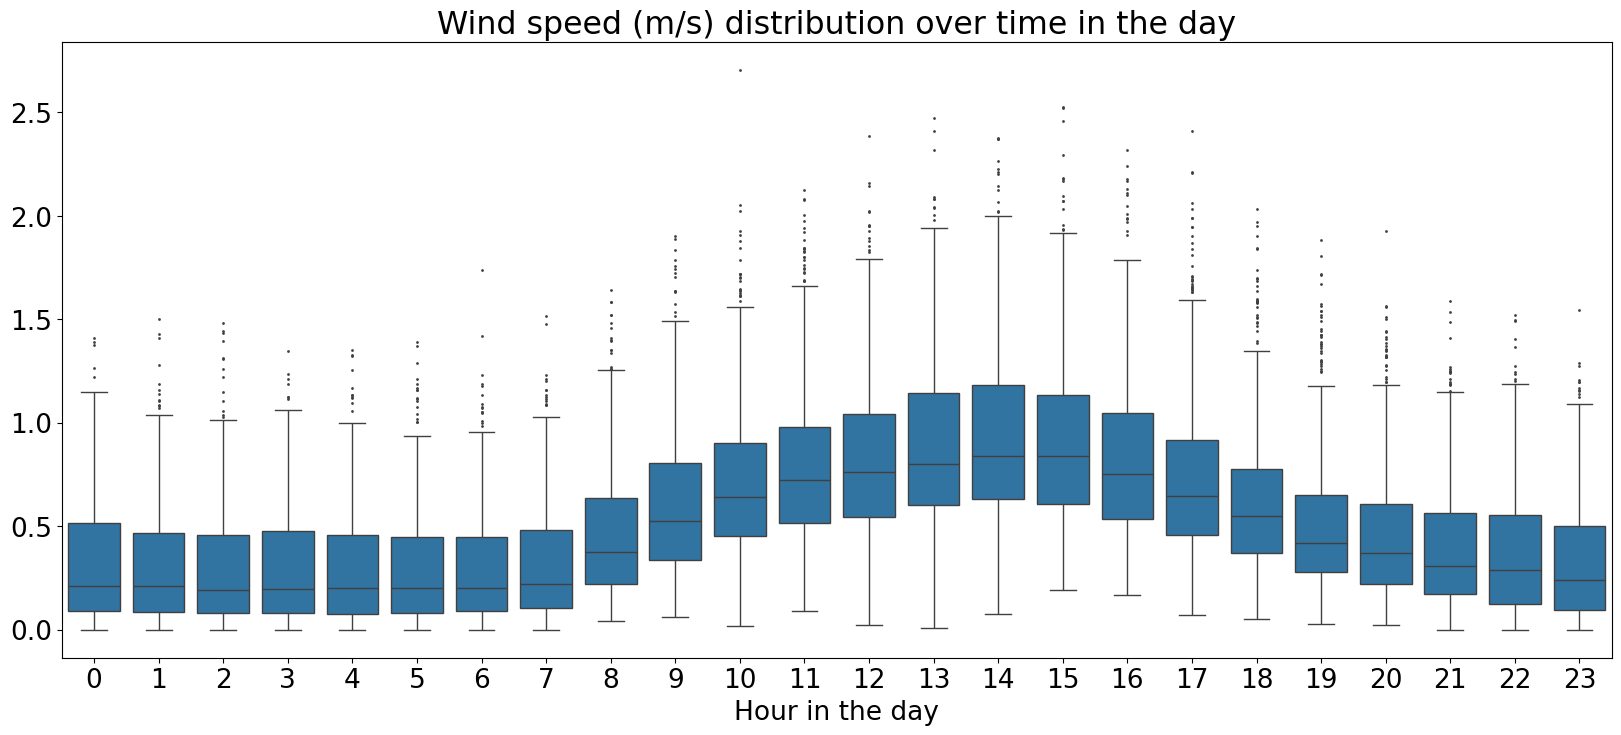
\includegraphics[scale=0.35]{figs/new_figs/wsboxplot.png}
	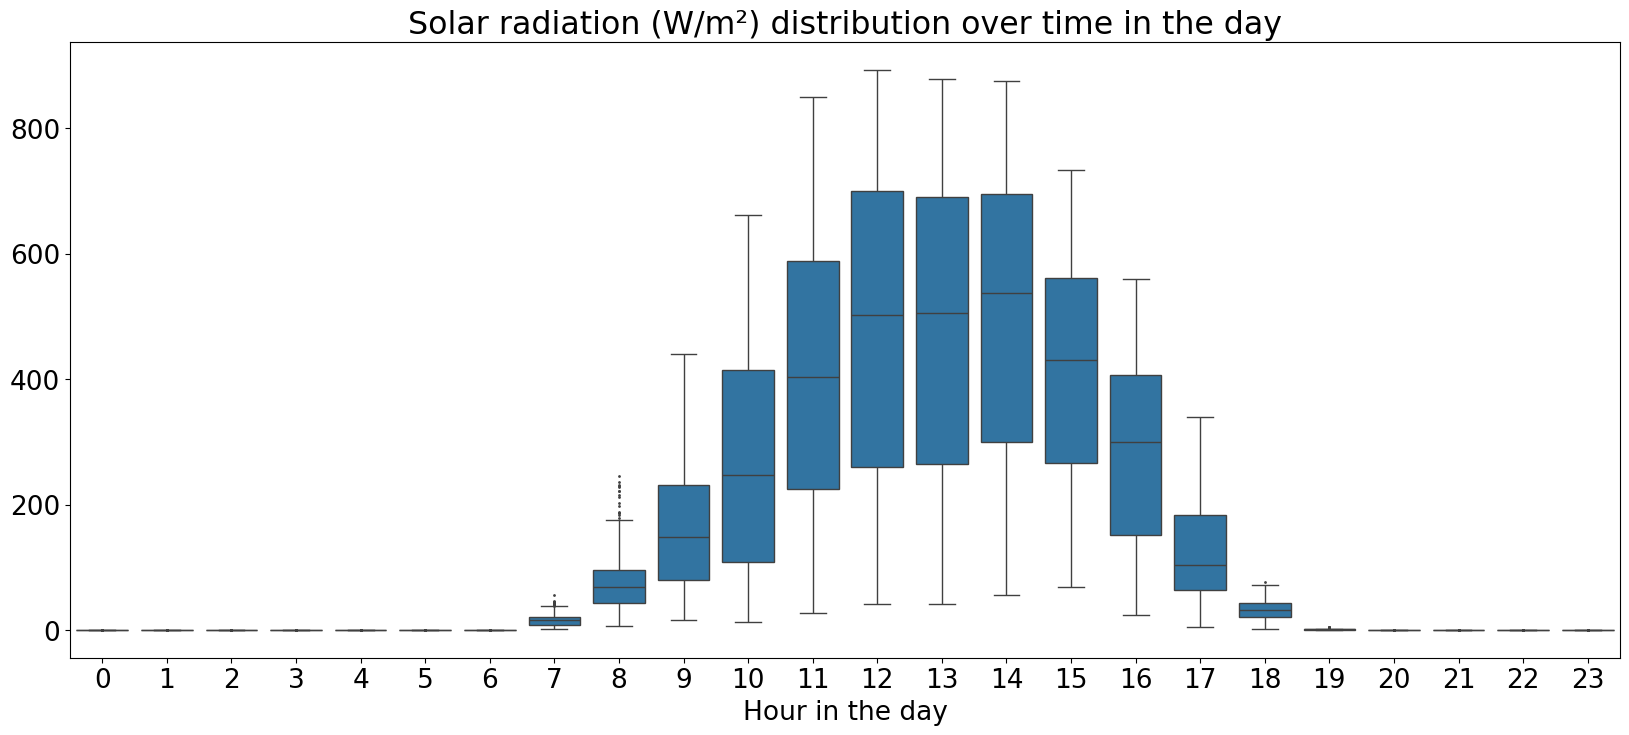
\includegraphics[scale=0.35]{figs/new_figs/srboxplot.png}
	\caption{Weather data distribution over time in the day.}
	\label{FIG:srbox}
\end{figure}
\fi

\iffalse 
\subsection{Case Study}

In Section \ref{Results}, we demonstrated that the Geo-Kriging-LSTM model proposed in this paper can provide accurate microclimate prediction results at high spatial resolutions. However, considering the computational complexity of the model itself, resource consumption is a concern. Therefore, we will discuss in this section that the model proposed in this paper, along with the associated theories, can be applied in a broader context. In order to discuss the generalizability, we designed several scenarios.

To evaluate the marginal loss of reducing additional weather stations, we apply our prediction model to different scales of datasets. The scenarios are summarized as follows:
\begin{itemize}
    \item Neighbors5: Using 5 nearest other stations for training
    \item Neighbors3: Using 3 nearest other stations for training
    \item LULC-Neighbor3: Using 3 stations, whose LULC are the closest to the target station, of the 5 nearest other stations
\end{itemize}

From these experiments, we found that removing weather data from stations with different LULCs can less affect the model's performance, which means the weather data is most affected by the neighbor stations with similar LULCs. On the contrary, this result also guides us that the new stations placed at locations with different LULCs can gain the maximal information. Figure \ref{FIG:different_station_placement} shows the error evaluation of the three models in the experiments. The performance of LULC-Neighbor3 is closer to the performance of Neighbor5, which means the information from the stations dropped in LULC-Neighbor3 is less than the stations dropped in Neighbor3. These experimental results indicate that our model can save computational resources by observing the similarity in LULC data. In practice, we can select a few weather stations with similar LULC data and close geographic characteristics as interpolation targets. Using the model proposed in this paper for predictions, the results can meet the accuracy requirements in general applications. Furthermore, these experimental results can also provide a theoretical basis to some extent for the selection of urban weather station locations. Setting neighboring meteorological stations in locations with significantly different geographic characteristics can provide the maximum information for extracting microclimate knowledge. 
\fi

\iffalse
\begin{figure}[!h]
	\centering
	\includegraphics[scale=0.6]{figs/different_placement4.png}
	\caption{Comparison of different station settings.}
	\label{FIG:different_station_placement}
\end{figure}
\fi

In addition to the discussed applications, our predictions of microclimates can assist various research problems. Besides the traditional studies mentioned in the related work section, such as high-precision BPS, thermal comfort, residents' health, and building material lifespan, the predictions in high-spatial and high-temporal dimensions can aid in establishing urban or district digital twins. That is, these predictions provide real-time and high-resolution input to support digital twins, enabling simulations and achieving a feedback loop with the real-world, which is currently often missing~\citep{2023_autcon_dt_challenges,2023_scs_human_dt}. 


This study proposes a novel microclimate prediction model, the LSTM-Kriging model, which combines both temporal and spatial knowledge. Furthermore, this model incorporates LULC through the Geo-LSTM-Kriging model to adapt to the influences of urban environmental obstacles. Our experiment results demonstrate the effectiveness of this methodology in a range of actual cases, particularly in moments with dramatic environmental changes.

Compared to past research, the model proposed in this paper has several innovative aspects. Firstly, our predictions achieve a spatial resolution of 1 meter, whereas \cite{di2020mean} using NWP to obtain prediction results with a spatial resolution of 2.5 x 2.5 km, \cite{chang2021development} developing a UMTF model to predict the microclimate with a spatial resolution of 50 x 50 m. This significant improvement in spatial resolution is of meaningful significance for studies that require higher microclimate spatial density. Besides, our approach provides a new perspective on weather prediction models, particularly in scenarios with environmental variations. \cite{erell2022effect} indicated that achieving a green surface proportion of 0.5 would result in a decrease of approximately 0.3\textdegree C in the annual average temperature. Our analysis of the impact of LULC data shows that considering LULC data reduces the MAE from 0.61\textdegree C to 0.12\textdegree C, which further confirms the significance of considering environmental conditions on the microclimate. This ability to adapt to urban environmental obstacles makes our model a valuable tool for weather prediction in urban environments. Additionally, traditional research often relies on directly using data from neighboring weather stations or classic weather files \citep{kruger2013assessment,kruger2017identifying,li2020perception}, which can be insufficiently accurate in certain microclimate studies. The model proposed in this study offers temperature and humidity predictions for microclimates with spatial resolution and achieves better performance compared with weather stations and weather files. At the same time, the data required for this method is widely and freely available at a sufficient level of quality, e.g.\ from volunteered geographic information platforms such as OpenStreetMap~\citep{2023_bae_osm_qa,Herfort.2023}, allowing wide applicability.

%In contrast, our model offers temperature and humidity predictions for microclimates with spatial resolution. Furthermore, our model exhibits higher accuracy in areas surrounded by buildings or green spaces compared to traditional models. 



\section{Conclusion}\label{Conclusion}

This study proposes the LSTM-Kriging model, which combines both temporal and spatial knowledge to develop a novel weather interpolation model, enabling the prediction of microclimate conditions at a high resolution in the built environment. Our Geo-LSTM-Kriging model further incorporates LULC data to adapt to the influences of urban environmental obstacles. Our experiment results demonstrate the effectiveness of this methodology in a range of actual cases, particularly in moments with dramatic environmental changes. 

The study introduces several key findings:
\begin{itemize}
    \item Our approach provides an improvement over traditional microclimate prediction baselines, demonstrating the importance of incorporating spatial, temporal, and geographical knowledge (LULC) in the model. Compared to the direct use of urban weather station (Changi Airport) data, the temperature prediction RMSE of our high spatial-resolution model has reduced from 1.09\textdegree C to 0.64\textdegree C, the RH prediction RMSE has decreased from 6.73 to 3.23. While the traditional interpolation method (Kriging interpolation) yielded a temperature prediction RMSE of 1.59\textdegree C and an RH RMSE of 7.70. The addition of the Geo-layer helped reduce the prediction error of temperature from 0.70\textdegree C to 0.64\textdegree C and of humidity from 3.43 to 3.23.

    \item The analysis in the paper regarding the influence of different LULC data from various weather stations on the prediction results indicates that the extent of building and vegetation coverage in the environment can lead to varying degrees of impact on microclimate prediction during different time periods. The addition of Geo-layer allows for learning the impact of LULC features to some extent, enhancing the stability of the model predictions, especially during periods of significant fluctuations in the original data. For instance, the standard deviation of temperature prediction error at 13:00 reduced from 0.96 to 0.57.

    \item This study also conducted a temporal analysis of model errors for weather station clustering. It was observed that among various LULC features, terrain, distance to buildings, and distance to walkways might influenced more on the model performance.
    
\end{itemize} 

However, the study also identifies some limitations and a few open questions remain. Our experiments implemented for the Geo-LSTM-Kriging model are restricted to a small area with only 14 weather stations, hence, the analysis and conclusions drawn from the clustering results are highly limited. Furthermore, the model does not consider the effect of vertical dimension, which may not be a negligible factor when considering geographical information. Additionally, there are some typical features that are also crucial for microclimate research, such as wind speed, solar radiation, etc. This paper primarily focuses on discussing temperature and RH, with the expansion to other features expected to be explored in future research. Despite these limitations, because of the notable advancements in performance, we believe that our study provides a contribution to the field of weather forecasting in urban environments, which could be further improved and applied to specific tasks.

Future research should focus on expanding the model's applicability to other geographical locations and scaling it to larger areas, and incorporating more comprehensive data, such as classified point cloud data and street-level imagery, which may add further value to the predictions thanks to their high resolution and additional information~\citep{Megahed2021,2023_jag_svi_sensitivity}. Moreover, the form of the employment of geographical information could be explored beyond the convolution-like layer structure proposed in this study. With these improvements, the proposed model could be a valuable tool for weather forecasting and urban planning.

\section*{Data availibility}
The research compendium for this article can be found at \url{https://github.com/ideas-lab-nus/microclimate-dl-predict}, hosted at Github.

\section*{Acknowledgements}

This research project is supported by the Singapore Ministry of Education Academic Research Fund (MOE-ARF) Tier 1 (grant number A-8000139-00-00); the National Research Foundation, Singapore, and Ministry of National Development, Singapore under its Cities of Tomorrow R\&D Programme (CoT Award COT-V4-2020-5). We thank Dr. Marcel Ignatius for his initial input and support in the early stages of this study. 


\printcredits

%% Loading bibliography style file
% \bibliographystyle{model1-num-names}
\bibliographystyle{cas-model2-names}

% Loading bibliography database
\bibliography{cas-refs}




%\vskip3pt

\end{document}
%!!!appendix_start
\section{Methods Comparison Tables}

%Appendix sections are coded under \verb+\appendix+.

\begin{figure}[!h]
	\centering
	\includegraphics[scale=0.45]{figs/RH_14STATIONS2.png}
	\caption{Mean relative absolute error and R squared of RH at all stations.}
	\label{FIG:RH_5Stations}
\end{figure}
\begin{figure}[!h]
	\centering
	\includegraphics[scale=0.45]{figs/TEM_14STATIONS2.png}
	\caption{Mean relative absolute error and R squared of temperature at all stations.}
	\label{FIG:TEM_5Stations}
\end{figure}



\begin{table}
\caption{Comparison of the Geo-LSTM-Kriging methods given different scale of sensors.}\label{use case of weather sensor placement description2}
\begin{tabular*}{\tblwidth}{@{} LLLLLLLL@{} }
\toprule
Station number &  1 & 2 & 3 & 4 & 5&  6 & 7\\
\midrule
True RH mean value & 72.83 & 70.79 & 70.86 & 71.37 & 73.15& 74.62 & 71.59\\
%Nearest4 MAE & 4.63& 3.42& 3.31& 3.3& 4.72& 3.32& 3.23\\
Neighbors5 MAE &3.19&3.24&1.69&4.43&3.16&2.34&2.28\\
Neighbors3 MAE & 3.97 &3.76 &5.73&5.48&3.34& 4.26 &4.52\\
LULC-Neighbors3 MAE & 4.78& 4.98 &4.34 & 4.57 & 5.72& 5.45& 3.23\\
Neighbors3 MRE increased &33.26\%&34.94\%&61.06\%&3.06\%&44.76\%&57.06\%&29.41\%\\
Geo-Neighbors3 MRE increased &16.95\%&24.50\%&32.03\%&19.91\%&41.60\%&21.83\%&39.94\%\\
\bottomrule
\end{tabular*}
\begin{tabular*}{\tblwidth}{@{} LLLLLLLL@{} }
\toprule
Station number  & 8 & 9 & 10&11 &12 &13 &14\\
\midrule
True RH mean value  & 92.63 & 73.39 & 73.26&86.7&82.4&78.3&77.1\\
%Nearest4 MAE & 10.45& 3.42& 5.56&4.43&3.76&4.24&3.87\\
Neighbors5 MAE  &8.25&3.72&4.26&4.52&3.35&3.24&3.21\\
Neighbors3 MAE  &10.87&5.58&5.62&4.96&4.07&3.85&3.58\\
LULC-Neighbors3 MAE &11.10 & 5.34 & 4.28&4.21&3.32&3.94&3.64\\
Neighbors3 MRE increased & 25.68\%&30.34\%&0.47\%&7.36\%&0.90\%& 17.77\%&11.81\%\\
Geo-Neighbors3 MRE increased & 2.07\%&4.50\%&31.31\%&17.81\%&22.59\%& 2.28\%&1.65\%\\
\bottomrule
\end{tabular*}
\end{table}


\begin{figure}[!h]
	\centering
	\includegraphics[scale=0.3]{figs/timeseries_S1_7_RH.png}
    
	\caption{MAE and Std. of RH at stations 1 to 7. The horizontal axis denotes the time of the day, the mean is taken over one hour}
	\label{FIG:TIMEanalysis}
\end{figure}
\begin{figure}[!h]
	\centering
	\includegraphics[scale=0.3]{figs/timeseries_S8_14_RH.png}
	\caption{MAE and Std. of RH at stations 8 to 14. The horizontal axis denotes the time of the day, the mean is taken over one hour.}
	\label{FIG:TIMEanalysis2}
\end{figure}
\begin{figure}[!h]
	\centering
	\includegraphics[scale=0.3]{figs/timeseries_S1_7_Tem.png}
	\caption{MAE and Std. of temperature at stations 1 to 7. The horizontal axis denotes the time of the day, the mean is taken over one hour.}
	\label{FIG:TIMEanalysis3}
\end{figure}
\begin{figure}[!h]
	\centering
	\includegraphics[scale=0.3]{figs/timeseries_S8_14_Tem.png}
	\caption{MAE and Std. of temperature at stations 8 to 14. The horizontal axis denotes the time of the day, the mean is taken over one hour.}
	
 
 
 
 
 \label{FIG:TIMEanalysis4}
\end{figure}

\begin{figure}[!h]
	\centering
	\includegraphics[scale=0.5]{figs/variance2.png}
	\caption{The 24-hour average Std. of the two models.}
	\label{FIG:variance}
\end{figure}
%!!!appendix_end

\begin{table}[width=.9\linewidth,cols=4,pos=h]
\caption{Comparison of the improvement given by different layers.}\label{comparison of the improvement given by different layers}
\begin{tabular*}{\tblwidth}{@{} LLLLLLLL@{} }
\toprule
Station number &  1 & 2 & 3 & 4 & 5& 6 & 7\\
\midrule
True RH mean value & 72.83 & 70.79 & 70.86 & 71.37 & 73.15& 74.62 & 71.59\\
LSTM-linear prediction MAE & 5.63& 8.42& 8.31& 5.3& 7.72& 5.37& 4.25\\
Kriging prediction MAE & 12.78& 11.98 &12.34 & 11.57 & 8.72& 10.85& 11.56\\
LSTM-Kriging prediction MAE & 4.97 &4.76 &6.73&7.48&6.34& 4.51 &4.35\\
Geo-LSTM-Kriging prediction MAE  &4.19&4.24&2.69&6.43&6.16& 3.32& 3.23\\
LSTM-layer MRE improvement & 10.72\%&10.20\%&7.92\%&5.70\%&3.25\%& 8.64\%&8.38\%\\
Kriging-layer MRE improvement & 0.87\%&5.14\%&2.21\%&-3.18\%&1.86\%& 2.19\%&5.25\%\\
Geo-layer MRE improvement&1.07\%&1.06\%&5.69\%&1.46\%&0.24\%&1.05\%&1.34\%\\
\midrule
True temperature mean value($^\text{o}$C) & 29.20 & 29.52 & 29.30 & 29.50 &28.91& 29.44 & 29.24\\
LSTM-linear prediction MAE &1.0826&1.2971&1.1335&1.8742&1.6646&1.0346&1.4583 \\
Kriging prediction MAE &1.3492&1.3882&1.4265&2.0884&1.8759&1.3528&1.7332 \\
LSTM-Kriging prediction MAE & 0.9079&1.2105&1.1174&1.8124&1.6309& 0.9142&1.2519\\
Geo-LSTM-Kriging prediction MAE &0.9464&1.2511&1.0236&1.8062&1.5260&0.9324&1.2021\\
LSTM-layer MRE improvement & 1.51\%&0.60\%&1.05\%&0.94\%&0.85\%& 1.37\%&0.71\%\\
Kriging-layer MRE improvement&0.59\%&0.29\%&0.095\%&0.21\%&0.12\% &0.58\%&0.38\%\\
Geo-layer MRE improvement&-0.13\%&-0.14\%&0.32\%&0.02\%&0.36\%&0.15\%&0.17\%\\
\bottomrule
\end{tabular*}
\begin{tabular*}{\tblwidth}{@{} LLLLLLLL@{} }
\toprule
Station number & 8 & 9 & 10 &  11 & 12 & 13 & 14\\
\midrule
True RH mean value  & 92.63 & 73.39 & 73.26& 83.34 & 76.96 & 82.35 & 74.67\\
LSTM-linear prediction MAE & 18.54& 4.34& 7.61& 6.26& 4.54& 8.46& 4.62\\
Kriging prediction MAE  &20.42 & 10.83 & 9.24& 10.76& 11.06 &9.87 & 10.35\\
LSTM-Kriging prediction MAE  &12.32&5.17&5.69& 4.18 &3.37 &3.54&3.05\\
Geo-LSTM-Kriging prediction MAE& 10.45& 3.42& 5.56 & 3.59& 3.17& 2.56& 2.59\\
LSTM-layer MRE improvement &9.35\%&4.24\%&4.36\%&8.31\%&8.92\%&9.13\%&5.76\%\\
Kriging-layer MRE improvement &2.41\%&3.02\%&1.57\%& 4.95\%&3.96\%&1.84\%&5.02\%\\
Geo-layer MRE improvement&4.73\%&2.04\%&0.56\%&1.05\%&2.16\%&3.23\%&1.58\%\\
\midrule
True temperature mean value($^\text{o}$C)  & 28.34 & 29.65 &29.12& 29.44 & 29.24 & 28.34 & 29.65\\
LSTM-linear prediction MAE &1.3774&1.6923&1.4036&1.1756&1.0646&1.239&1.785 \\
Kriging prediction MAE &1.5941&1.9538&1.8306&1.7464&1.8571&1.6969&1.8723  \\
LSTM-Kriging prediction MAE &1.1238&1.8301&1.8826 & 1.0413&1.0569&1.2512&1.7764\\
Geo-LSTM-Kriging prediction MAE &1.0583&1.7239&1.5101&0.9529&0.8724&0.8564&1.2274\\
LSTM-layer MRE improvement &1.21\%&0.85\%&0.64\%& 1.54\%&0.96\%&1.47\%&1.63\%\\
Kriging-layer MRE improvement&0.07\%&0.11\%&0.35\%&0.58\%&0.54\%&0.82\%&0.65\% \\
Geo-layer MRE improvement&0.28\%&0.12\%&0.18\%&0.27\%&0.36\%&0.54\%&0.76\%\\
\bottomrule
\end{tabular*}
\end{table}




g^i&=\frac{1}{\text{number of neighbor points}}\sum_{j\in\{\text{neighbor points of station }i\}}\bold{1}(j\text{ is in the shadow of a building or tree})